\documentclass[11pt,oneside]{book}
\usepackage{fontspec}
\setmainfont{Noto Serif}
\setsansfont{Noto Sans}
\setmonofont{Noto Sans Mono}
\newfontfamily\proseunicodefont{DejaVu Serif}
\usepackage[margin=1in]{geometry}
\usepackage{microtype}
\usepackage{amsmath,amssymb,amsthm,mathtools,bm}
\usepackage{graphicx}
\usepackage{xcolor}
\usepackage{booktabs}
\usepackage{array}
\usepackage{longtable}
\usepackage{enumitem}
\usepackage{float}
\usepackage{caption}
\usepackage{hyperref}
\usepackage{fancyhdr}
\usepackage{tikz}
\usetikzlibrary{arrows.meta,positioning,calc,decorations.pathmorphing}

\hypersetup{
  colorlinks=true,
  linkcolor=blue!50!black,
  urlcolor=blue!50!black,
  citecolor=blue!50!black
}

\setlength{\parskip}{0.5em}
\setlength{\parindent}{0pt}
\setlist[itemize]{topsep=0.25em,itemsep=0.2em}
\setlist[enumerate]{topsep=0.25em,itemsep=0.2em}
\setlength{\headheight}{40pt}
\numberwithin{equation}{chapter}

\newtheorem{theorem}{Satz}[chapter]
\newtheorem{proposition}[theorem]{Proposition}
\newtheorem{lemma}[theorem]{Lemma}
\newtheorem{corollary}[theorem]{Korollar}
\theoremstyle{definition}
\newtheorem{definition}[theorem]{Definition}
\newtheorem{example}[theorem]{Beispiel}
\theoremstyle{remark}
\newtheorem{remark}[theorem]{Bemerkung}

\providecommand{\ket}[1]{\left\lvert#1\right\rangle}
\providecommand{\bra}[1]{\left\langle#1\right\rvert}
\providecommand{\braket}[2]{\left\langle#1\,\middle|\,#2\right\rangle}
\providecommand{\expect}[1]{\left\langle#1\right\rangle}
\newcommand{\lectureoverview}[1]{\paragraph{Überblick.} #1}
\newenvironment{classroomqa}{%
  \par\medskip
  \begin{minipage}{0.96\textwidth}
}{%
  \end{minipage}
  \par\medskip
}
\newcommand{\audiencequestion}[1]{\noindent\textbf{Frage aus dem Publikum.} #1\par\smallskip}
\newcommand{\lecturerresponse}[1]{\noindent\textbf{Antwort.} #1\par}
\newcommand{\lecturetimestamp}[1]{\footnote{Vorlesungszeit: #1.}}
\newcommand{\lectureframe}[1]{\par\smallskip{\centering\footnotesize\itshape Vorlesungsbild: #1.\par}}
\newcommand{\editorialnote}[1]{\footnote{Redaktionelle Klarstellung: #1}}

\makeatletter
\newcommand{\course@headerfont}{\normalfont\small\itshape}
\newcommand{\course@pagefont}{\normalfont\small}
\newcommand{\course@headerraise}{14pt}
\newlength{\course@headerboxheight}
\setlength{\course@headerboxheight}{\dimexpr\headheight-\course@headerraise-9pt\relax}
\newcommand{\course@leftheadbox}[1]{%
  \raisebox{\course@headerraise}{%
    \parbox[t][\course@headerboxheight][t]{0.82\textwidth}{%
      \raggedright\course@headerfont\strut\MakeUppercase{#1}\strut%
    }%
  }%
}
\newcommand{\course@rightheadbox}[1]{%
  \raisebox{\course@headerraise}{%
    \parbox[t][\course@headerboxheight][t]{0.82\textwidth}{%
      \raggedleft\course@headerfont\strut\MakeUppercase{#1}\strut%
    }%
  }%
}
\renewcommand{\chaptermark}[1]{\markboth{\MakeUppercase{\chaptername\ \thechapter.\ #1}}{}}
\renewcommand{\sectionmark}[1]{\markright{\MakeUppercase{\thesection\hspace{0.4em}#1}}}
\fancyhf{}
\fancyhead[L]{\course@leftheadbox{\leftmark}}
\fancyhead[R]{\course@pagefont\thepage}
\renewcommand{\headrulewidth}{0.5pt}
\pagestyle{fancy}
\fancypagestyle{plain}{%
  \fancyhf{}
  \fancyhead[L]{\course@leftheadbox{\leftmark}}
  \fancyhead[R]{\course@pagefont\thepage}
  \renewcommand{\headrulewidth}{0.5pt}
}
\makeatother

\usepackage{polyglossia}
\setdefaultlanguage{german}
\usepackage{sectsty}
\renewcommand{\contentsname}{Inhaltsverzeichnis}
\renewcommand{\chaptername}{Kapitel}
\renewcommand{\figurename}{Abbildung}
\renewcommand{\tablename}{Tabelle}
\renewcommand{\proofname}{Beweis}
\renewcommand{\bibname}{Literatur}
\sectionfont{\raggedright}
\subsectionfont{\raggedright}
\makeatletter
\renewcommand{\@pnumwidth}{2.2em}
\renewcommand{\@tocrmarg}{3.2em}
\makeatother
\usepackage{tocloft}
\renewcommand{\cftchapfont}{\small\bfseries}
\renewcommand{\cftchappagefont}{\small\bfseries}
\renewcommand{\cftsecfont}{\small}
\renewcommand{\cftsecpagefont}{\small}
\setlength{\cftsecnumwidth}{3em}
\renewcommand{\cftsubsecfont}{\small}
\renewcommand{\cftsubsecpagefont}{\small}
\setlength{\cftsubsecindent}{4.5em}
\setlength{\cftsubsecnumwidth}{4em}
\emergencystretch=6em
\pdfstringdefDisableCommands{\def\proseunicodefont{}}

\geometry{paperwidth=177.6mm,paperheight=252mm,left=16mm,right=16mm,
 top=18mm,bottom=18mm,includeheadfoot,headheight=28pt,headsep=7mm,footskip=9mm}
\usepackage{scrextend}
\changefontsizes[17pt]{12pt}
\raggedbottom
\renewenvironment{classroomqa}{\par\medskip\begingroup}{\par\endgroup\medskip}
\fancyhf{}
\setlength{\headwidth}{\textwidth}
\fancyhead[L]{\parbox{\textwidth}{\raggedright\fontsize{9}{11}\selectfont\nouppercase{\leftmark}}}
\fancyfoot[C]{\small\thepage}
\renewcommand{\headrulewidth}{0.3pt}
\fancypagestyle{plain}{\fancyhf{}\fancyfoot[C]{\small\thepage}\renewcommand{\headrulewidth}{0pt}}

\hypersetup{
  pdftitle={Quantum Entanglement, Part 3},
  pdfauthor={Lectures by Leonard Susskind; companion edition by LazyingArt LLC},
  pdfsubject={Independently edited companion notes for the 2006 Fall lecture course},
  pdfcreator={LaTeX with hyperref}
}
\graphicspath{{../../../generated_course_notes/supplementary/quantum_entanglement/2006_fall_part_3/figures/}{../../../generated_course_notes/supplementary/quantum_entanglement/2006_fall_part_3/assets/}}
\begin{document}
\frontmatter
\hypersetup{pageanchor=false}
\begin{titlepage}
\hyphenpenalty=10000\exhyphenpenalty=10000
\thispagestyle{empty}
\begin{tikzpicture}[remember picture,overlay]
  \node[anchor=center,inner sep=0] at (current page.center) {%
    \includegraphics[height=\paperheight,keepaspectratio]{../../../generated_course_notes/supplementary/quantum_entanglement/2006_fall_part_3/assets/cover-art.png}%
  };
  \node[
    anchor=north west,
    align=left,
    text width=0.78\paperwidth,
    fill=white,
    fill opacity=0.9,
    rounded corners=8pt,
    inner xsep=10pt,
    inner ysep=8pt
  ] at ([xshift=0.08\paperwidth,yshift=-0.06\paperheight]current page.north west) {%
    {\fontsize{30}{33}\selectfont\bfseries\color{black!88} Quantenverschränkung, Teil 3\\[0.85em]}
    {\large\color{black!72} Deutsche Ausgabe / Herbst 2006, Teil 3}
  };
  \node[
    anchor=south west,
    align=left,
    text width=0.68\paperwidth,
    fill=white,
    fill opacity=0.82,
    text opacity=1,
    rounded corners=6pt,
    inner sep=12pt
  ] at ([xshift=0.08\paperwidth,yshift=0.08\paperheight]current page.south west) {%
    {\normalsize\color{black!78} Originalvorlesungen: Leonard Susskind\\[0.35em]}
    {\small\color{black!72} Begleitausgabe: \href{https://lazying.art}{LazyingArt LLC} / \href{https://github.com/lachlanchen/Video2Book}{Video2Book}}
  };
\end{tikzpicture}
\mbox{}
\end{titlepage}
\hypersetup{pageanchor=true}

\clearpage
\chapter{Über diese Notizen}
Diese unabhängig redigierten Begleitnotizen folgen dem dritten Teil von Leonard Susskinds Vorlesungskurs zur Quantenverschränkung aus dem Jahr 2006. Sie wurden anhand maschineller Transkripte, Untertitel und ausgewählter Tafelbilder rekonstruiert und anschließend mit dem verfügbaren Quellenmaterial abgeglichen. Sie sind kein Originalmanuskript von Professor Susskind und wurden von ihm weder geprüft noch autorisiert.

Die Ausgabe wurde von \href{https://lazying.art}{LazyingArt LLC} mit dem quelloffenen Werkzeug \href{https://github.com/lachlanchen/Video2Book}{Video2Book} erstellt. Maschinelle Transkripte sind separat verfügbar und können Erkennungsfehler enthalten. Redaktionelle Klarstellungen und nichttriviale Rekonstruktionen sind in Fußnoten gekennzeichnet.
\clearpage
\tableofcontents
\mainmatter
\chapter{Spezielle Relativitätstheorie: Bezugssysteme, Gleichzeitigkeit und die Lorentz-Transformation}

Relativität ist das Prinzip, dass die Gesetze der Physik nicht davon abhängen, welches Inertialsystem wir zu ihrer Beschreibung verwenden. Unsere erste Aufgabe ist die Kinematik: die Bedeutung von Raum, Zeit, Bewegung, Synchronisation und der Transformation von einem Inertialsystem in ein anderes. Danach folgt die Dynamik mit relativistischer Energie, relativistischem Impuls, Kraft, dem Analogon zu Newtons Bewegungsgleichung und der Bedeutung von \(E=mc^2\). Sobald dieses Gerüst gesichert ist, können wir uns der allgemeinen Relativitätstheorie konzeptionell über die gekrümmte Raumzeit, die Bewegung von Teilchen in einem vorgegebenen Gravitationsfeld, Schwarze Löcher und die Expansion des Universums nähern, ohne mit dem schwierigen Problem zu beginnen, Einsteins Feldgleichungen zu lösen.

Es lohnt sich, zwischen konzeptioneller und mathematischer Strenge zu unterscheiden. Wir werden keine Näherung verwenden, von der wir wissen, dass sie falsch ist. Stattdessen betonen wir, wie ein Gravitationsfeld auf Uhren, Teilchen und Geometrie wirkt, und verschieben die mathematischen Werkzeuge, die nötig sind, um beliebige Lösungen der Feldgleichungen zu konstruieren. Die spezielle Relativitätstheorie muss ausführlicher behandelt werden, weil alle späteren Überlegungen auf ihrer Kinematik beruhen.

Der richtige Ausgangspunkt ist daher nicht eine berühmte Formel, sondern eine präzise Darstellung dessen, was ein Beobachter unter einem Ort und einer Zeit versteht.

\section{Ein Bezugssystem ist ein physikalisches Koordinatensystem}

Stellen wir uns vor, der Raum sei mit einem beliebig feinmaschigen Gitter aus Meterstäben ausgefüllt. Jeder Gitterpunkt ist durch drei räumliche Koordinaten gekennzeichnet, und an jedem Punkt befindet sich eine Uhr. Zusammen bilden Stäbe und Uhren ein Bezugssystem.

\begin{definition}Ein \emph{Ereignis} ist etwas, das an einem Ort und zu einer Zeit geschieht. In einer räumlichen Dimension schreibt man seine Koordinaten als \((x,t)\), in drei Dimensionen als \((x,y,z,t)\).
\end{definition}

Die Newtonsche Physik fügt eine weitreichende Annahme hinzu: Alle idealen Uhren lassen sich ein für alle Mal synchronisieren. Die Zeit ist universell. Eine Uhr kann bewegt werden, und ein Beobachter kann eine Taschenuhr bei sich tragen, doch alle sollen überall dieselbe \(t\) angeben. Dies nennt man mitunter absolute Zeit; man kann sie sich als Gotteszeit vorstellen, als eine einzige Uhr für die ganze Welt.

Das Relativitätsprinzip ist älter als Einstein. Ein anschauliches Bild dafür ist ein Zug, der sich so gleichmäßig auf vollkommen glatten Schienen bewegt, dass nichts rattert oder wackelt. Im Zug können wir Bälle genauso zuwerfen und auffangen wie in einem Zug, der am Bahnhof steht. Jonglieren ist ein erstaunlich vollständiges kleines Mechanikexperiment: Es erfordert Zeitmessung, Schwerkraft, Ausrichtung und wiederholte Kontrolle von Flugbahnen. Bewegt sich der Zug mit konstanter Geschwindigkeit, ändert sich keine dieser Regeln. Ein senkrecht nach oben geworfener Ball kehrt in dieselbe Hand zurück; der Zug gleitet nicht unter ihm weg. Galileo erkannte diesen Sachverhalt, und Newton brachte ihn systematisch in seinen Bewegungsgesetzen zum Ausdruck.

Vor Galileo lag der Gedanke nahe, der fahrende Zug müsse während des Fluges des Balls weiterfahren, sodass der Jongleur die Hand nach hinten oder vorn bewegen müsse, um ihn wieder aufzufangen. Der Fehler dabei ist, zu vergessen, dass der Ball beim Verlassen der Hand bereits die horizontale Geschwindigkeit des Zuges besitzt. Kein Experiment, das auf den gleichmäßig fahrenden Wagen beschränkt ist, kann einen besonderen Zustand absoluter Ruhe nachweisen. Beobachtbar ist nur die Relativbewegung zwischen den beiden Zügen.

Der stehende und der sich gleichförmig bewegende Zug sind daher zwei Inertialsysteme. Vor Einstein waren sie durch Galilei-Transformationen miteinander verknüpft.

\section{Raumzeit zeichnen}

Zunächst lassen wir \(y\) und \(z\) weg und tragen die Zeit vertikal und den Ort \(x\) horizontal auf. Jeder Punkt in der Zeichnung ist ein Ereignis. Die Linie \(x=0\) ist die Geschichte oder die \emph{Weltlinie} des räumlichen Ursprungs. Die benachbarten vertikalen Linien \(x=1,2,3,\ldots\) sind die Weltlinien der übrigen Gitterpunkte. Horizontale Linien umfassen Ereignisse mit gleicher Zeit.

\begin{figure}[H]
\centering
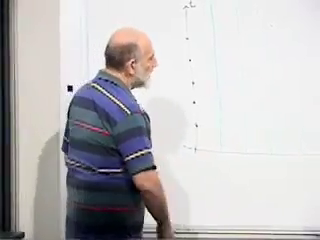
\includegraphics[width=0.62\textwidth]{lecture_01_figure_02.png}
\caption{Die Zeitachse des Ruhesystems und die ersten Weltlinien des räumlichen Gitters.}
\lectureframe{00:16:38}
\end{figure}

Dieselbe Konstruktion lässt sich in einer idealisierten Zeichnung anschaulicher darstellen:

\begin{figure}[H]
\centering
\begin{tikzpicture}[scale=0.95]
\draw[->] (-1.2,0) -- (5.2,0) node[right] {$x$};
\draw[->] (0,-0.2) -- (0,4.8) node[above] {$t$};
\foreach \x in {-1,1,2,3,4}
  \draw[gray!65] (\x,0) -- (\x,4.4);
\foreach \y in {1,2,3,4}
  \draw[gray!65] (-1.0,\y) -- (4.4,\y);
\fill (0,0) circle (1.5pt);
\node[below left] at (0,0) {$0$};
\node[left] at (0,1) {$1$};
\node[left] at (0,2) {$2$};
\node[left] at (0,3) {$3$};
\node[below] at (1,0) {$1$};
\node[below] at (2,0) {$2$};
\node[below] at (3,0) {$3$};
\end{tikzpicture}
\caption{Ein ruhendes Raumzeitgitter. Vertikale Linien haben konstanten Ort, horizontale Linien konstante Zeit.}
\end{figure}

Das Gitter ist imaginär, und sein Abstand ist beliebig. Wir können Meter, Zentimeter, Mikrometer oder ein noch kleineres Intervall verwenden, sofern es physikalisch sinnvoll ist. Es dient dazu, jedem Ereignis eine präzise Koordinate zuzuordnen.

Der Begriff „Bezugssystem“ hat nun eine operationale Bedeutung. Er bezeichnet nicht bloß einen Standpunkt oder eine Person, die in eine bestimmte Richtung blickt, sondern einen ausgedehnten Koordinatenapparat. Zu einem Ereignis geben die örtlichen Stäbe an, wo es stattgefunden hat, und die örtliche Uhr, wann. Dann lassen sich auch andere physikalische Größen zwischen Bezugssystemen vergleichen: der Ort und die Geschwindigkeit eines Teilchens, seine Energie, vielleicht die Temperatur eines Körpers und schließlich sein Impuls und die Kraft. Am einfachsten ist der Vergleich für \(x\) und \(t\); damit beginnen wir.

Nun bringen wir ein zweites Gitter auf einem Zug an, der sich in positiver \(x\)-Richtung mit konstanter Geschwindigkeit \(v\) bewegt. Wir wählen die Ursprünge so, dass sie bei \(t=0\) zusammenfallen. Der bewegte Ursprung folgt dann
\begin{equation}
x=vt.
\end{equation}
Jeder andere im Zug feste Punkt folgt einer parallelen, geneigten Weltlinie. Ihre Neigung bringt geometrisch lediglich zum Ausdruck, dass sich der Zug mit fortschreitender Zeit weiterbewegt.

Nehmen wir an, der hintere Punkt des Zuges sei der gestrichene Ursprung. Bei \(t=0\) fällt er mit dem Ursprung am Bahnhof zusammen. Zu einem späteren Zeitpunkt \(t\) hat er im Bahnhofssystem die Koordinate \(vt\). Ein benachbartes Ereignis mit der Koordinate \(x\) liegt daher nur \(x-vt\) vom Zugursprung entfernt. Deshalb ergibt sich die Transformation als Subtraktion und nicht als beliebige algebraische Regel.

Seien \((x,t)\) die Koordinaten eines Ereignisses im Bahnhofssystem und \((x',t')\) seine Koordinaten im Zugsystem. Galileo und Newton halten an der universellen Zeit fest:
\begin{equation}
t'=t.
\end{equation}
Während der Zeit \(t\) rückt der bewegte Ursprung um \(vt\) vor. Der Abstand zwischen diesem Ursprung und dem Ereignis beträgt daher
\begin{equation}
x'=x-vt.
\end{equation}
Zusammen ergibt sich
\begin{align}
t'&=t, & x'&=x-vt.
\label{eq:galilean-forward}
\end{align}
Löst man nach den ungestrichenen Koordinaten auf, erhält man die inverse Transformation:
\begin{align}
t&=t', & x&=x'+vt'.
\label{eq:galilean-inverse}
\end{align}

\begin{figure}[H]
\centering
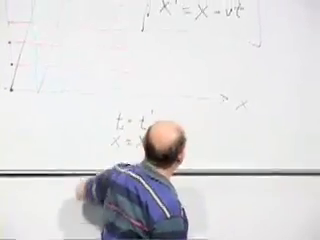
\includegraphics[width=0.72\textwidth]{lecture_01_figure_03.png}
\caption{Die Galilei-Transformation neben den beiden Raumzeitgittern.}
\lectureframe{00:21:57}
\end{figure}

Das erste Gleichungspaar gibt dem bewegten Beobachter an, wie er die Koordinaten des ruhenden Beobachters umrechnet. Das inverse Paar rechnet zurück. Diese wechselseitige Umrechnung der Beschreibungen ist der mathematische Gehalt der Galileischen Relativität.

Die Ersetzung \(t\to t'\) in der inversen Ortsformel ist nur deshalb unproblematisch, weil die Galileische Theorie bereits \(t=t'\) festgelegt hat. Es lohnt sich, diese Annahme jetzt zu beachten. In Einsteins Theorie werden die beiden Zeitkoordinaten verschieden sein, und solche Ersetzungen sind dann nicht mehr selbstverständlich.

\begin{classroomqa}
\audiencequestion{Wenn eine Uhr fortgetragen und dann zurückgebracht wird: Woher wissen wir, dass ihre Bewegung sie nicht zunächst vorgehen und dann nachgehen ließ, sodass der Effekt beim Uhrenvergleich verborgen bleibt?
\lecturetimestamp{00:23:09}}
\lecturerresponse{Galileo hätte die universelle Zeit nicht mit der Präzision moderner Methoden nachweisen können; sie war eine physikalische Vermutung. Wir können sie auf viele Arten prüfen: gute Uhren in entgegengesetzte Richtungen tragen, die Reise sowohl in Nord--Süd- als auch in Ost--West-Richtung wiederholen, eine Uhr um die andere herumführen oder Zeitsignale austauschen, ohne die Uhren zusammenzubringen. Bei gewöhnlichen Geschwindigkeiten stimmen all diese Tests mit sehr hoher Genauigkeit überein. Mit hinreichend genauen Uhren oder hinreichend großen Geschwindigkeiten zeigt sich eine kleine Abweichung. Das Versagen der universellen Zeit ist kein Mangel des Experiments, sondern eines der Phänomene, die die spezielle Relativitätstheorie erklären muss.}
\end{classroomqa}

\section{Galilei-Invarianten und Newtons Gesetz}

Eine Invariante ist eine Größe, über die alle betrachteten Inertialbeobachter übereinstimmen. Die Koordinaten selbst müssen nicht invariant sein. Entscheidend ist, ob die aus ihnen formulierten Gesetze ihre Gestalt behalten.

Das Wort wird sowohl als Substantiv als auch als Adjektiv verwendet. Eine Zahl kann eine Invariante sein, und eine Gleichung kann gegenüber einer Transformation invariant sein. Die Unterscheidung zwischen invarianten Größen und invarianten Gesetzen verhindert ein häufiges Missverständnis: Die Relativitätstheorie behauptet nicht, dass alle Beobachter für alles dieselbe Koordinate erhalten. Sie besagt, dass das physikalische Gesetz, das ihre Messungen verknüpft, dieselbe Form hat.

Betrachten wir zwei gleichzeitige Ereignisse an den Orten \(x_1\) und \(x_2\). Gleichung~\eqref{eq:galilean-forward} ergibt
\begin{align}
x_1'&=x_1-vt,\\
x_2'&=x_2-vt.
\end{align}
Ihr Abstand beträgt daher
\begin{equation}
x_2'-x_1'=(x_2-vt)-(x_1-vt)=x_2-x_1.
\end{equation}
In der Galileischen Physik ist der Abstand zwischen Ereignissen, die zur selben Zeit stattfinden, invariant, obwohl die einzelnen Orte es nicht sind.

\begin{classroomqa}
\audiencequestion{Sind die beiden Vorkommen von \(t\) in dieser Subtraktion wirklich dieselbe Zeit?
\lecturetimestamp{00:28:16}}
\lecturerresponse{Ja. Wir haben die beiden Ereignisse bewusst so gewählt, dass sie \((x_1,t)\) und \((x_2,t)\) sind. Sie liegen auf derselben horizontalen Linie konstanter Zeit. Der gemeinsame Term \(vt\) kürzt sich daher heraus. Fänden die Ereignisse zu unterschiedlichen Zeiten statt, wäre mit diesem Argument kein invariantes räumliches Intervall nachgewiesen.}
\end{classroomqa}

Beschreiben wir nun ein Teilchen durch eine Bahn \(x(t)\). Der Beobachter im Zug ordnet ihm zu:
\begin{equation}
x'(t)=x(t)-vt.
\end{equation}
Einmaliges Ableiten ergibt die bekannte Additionsregel für Geschwindigkeiten:
\begin{equation}
\frac{dx'}{dt}=\frac{dx}{dt}-v.
\end{equation}
Ort und Geschwindigkeit hängen vom Bezugssystem ab. Ein Beobachter, der neben einem Pfeil herfährt, sieht ihn langsamer fliegen als ein Beobachter, der neben der Strecke steht.

Leiten wir ein zweites Mal ab. Da die Relativgeschwindigkeit \(v\) konstant ist, gilt
\begin{equation}
\frac{d^2x'}{dt^2}=\frac{d^2x}{dt^2}.
\end{equation}
Die Beschleunigung ist unter einer Galilei-Transformation invariant. Das legt nahe, weshalb Newtons Gesetz mit der Beschleunigung und nicht mit Ort oder Geschwindigkeit formuliert wird.

Gemeint ist die Beschleunigung eines beobachteten Objekts, nicht die Beschleunigung des Zugbeobachters. Beide Bezugssysteme sind Inertialsysteme, also beschleunigt keines relativ zum anderen. Objekte können sich innerhalb beider Beschreibungen nach links oder rechts beschleunigen, und die beiden Beobachter stimmen im Wert dieser Beschleunigung überein, obwohl sie sich über den Ort und die Geschwindigkeit des Objekts uneinig sind.

Nehmen wir an, zwei Teilchen üben Kräfte aufeinander aus, und die Kraft hängt nur von ihrem gleichzeitigen Abstand ab. Dieser Abstand ist invariant, also ist auch die Kraft invariant. Wenn die Masse außerdem eine intrinsische, bezugssystemunabhängige Eigenschaft ist, kann jeder Inertialbeobachter schreiben:
\begin{equation}
F=ma
\end{equation}
und zwar genau in derselben Form. Die Newtonsche Mechanik ist unter Galilei-Transformationen invariant. Das ist nicht bloß plausibel; im Bereich gewöhnlicher Geschwindigkeiten ist sie außerordentlich genau.

Das Argument gilt für vertraute Zentralkräfte wie die Newtonsche Gravitation oder die Elektrostatik, deren Betrag eine Funktion des Abstands ist. Da alle Galilei-Beobachter bei gleicher Zeit in diesem Abstand übereinstimmen, stimmen sie auch in der Kraft überein. Wenn Kraft und Beschleunigung feststehen, müssen sie für Konsistenz auch in der Masse übereinstimmen: Ein Ein-Kilogramm-Objekt bleibt ein Ein-Kilogramm-Objekt, wenn es auf einem Zug an ihnen vorbeigetragen wird. Jedes Symbol in \(F=ma\) fügt sich in dieselbe invariante Struktur ein.

\section{Licht folgt nicht der Galileischen Regel}

Der Elektromagnetismus führt zu einer Schwierigkeit. Maxwells Gleichungen sagen Wellen voraus, die sich im leeren Raum mit einer bestimmten Geschwindigkeit \(c\) ausbreiten. Sind Maxwells Gleichungen Naturgesetze und gelten die Naturgesetze in jedem Inertialsystem in gleicher Form, dann müssen alle Inertialbeobachter denselben Wert für \(c\) erhalten.

Die Galileische Kinematik sagt etwas anderes voraus. Für einen nach rechts laufenden Lichtimpuls im ruhenden System gilt
\begin{equation}
x=ct.
\end{equation}
Wenden wir die Orts-Transformation an, ergibt sich
\begin{equation}
x'=x-vt=(c-v)t.
\end{equation}
Da \(t'=t\), würde der Zugbeobachter die Geschwindigkeit \(c-v\) messen.

Der Widerspruch lässt sich präzise formulieren. Wenn Maxwells Gleichungen ihre Form behalten, sagen sie im gestrichenen Bezugssystem \(c\) voraus. Behält man die Galilei-Transformation bei, ergibt sich dagegen \(c-v\). Wenn \(v\ne0\), können nicht beide Aussagen exakt sein.

Dieses Ergebnis erscheint völlig natürlich, wenn sich Licht wie eine gewöhnliche Welle in einem Medium verhält. Ein Boot, das sich mit einer Wasserwelle bewegt, misst eine geringere Relativgeschwindigkeit der Welle. Ein Beobachter, der sich durch ruhende Luft bewegt, misst eine Schallgeschwindigkeit, die sich aufgrund seiner Bewegung relativ zur Luft ändert. Physiker des 19. Jahrhunderts kamen daher auf einen bevorzugten Ruhezustand: ein Äthersystem, in dem Maxwells Gleichungen ihre einfachste Form haben und sich Licht mit \(c\) bewegt. Experimente, die eine Bewegung relativ zu diesem bevorzugten System nachweisen sollten, fanden keinen entsprechenden Effekt.

Es gab mehrere mögliche Versuchsanordnungen, doch allen lag dasselbe Ziel zugrunde: die Lichtausbreitung für Beobachter in unterschiedlichen Bewegungszuständen oder Bewegungsrichtungen zu vergleichen. Keine zeigte die erwartete Galileische Verschiebung. Das Scheitern war kein kleines technisches Ärgernis. Es zwang zu einer Entscheidung zwischen dem Relativitätsprinzip, Maxwells Gleichungen und den überlieferten Vorstellungen von Raum und Zeit.

Einstein ging den Konflikt unmittelbarer an. Als junger Mann stellte er sich vor, einer Lichtwelle nachzujagen. Könnte er sie einholen, würde ihr oszillierendes elektromagnetisches Muster im Raum stillstehen; Maxwells Gleichungen lassen jedoch keine solche stationäre Lichtwelle zu. Er entschied sich, Maxwells Theorie und das Relativitätsprinzip als grundlegend anzusehen und dann die in unseren Koordinaten verborgenen Annahmen neu zu überdenken.

Die Neuformulierung beruht auf zwei Postulaten:
\begin{enumerate}
\item Die Gesetze der Physik haben in jedem Inertialsystem dieselbe Form.
\item Licht im Vakuum hat in jedem Inertialsystem dieselbe Geschwindigkeit \(c\).
\end{enumerate}

Das zweite Postulat ist mit der Galilei-Transformation unvereinbar. Etwas Grundlegenderes als die Regel zur Addition von Geschwindigkeiten muss sich ändern. Einstein entscheidet sich auf ökonomische Weise dafür, die beiden Postulate beizubehalten und die scheinbar harmlose Galileische Gleichung \(t'=t\) neu zu überdenken.

\section{Entfernte Uhren synchronisieren}

Räumliche Abstände lassen sich mit Stäben festlegen, doch für entfernte Uhren braucht man eine Synchronisationskonvention. Man stelle zwei Uhren in gleichem Abstand von einem Beobachter in der Mitte auf. Wenn jede Uhr am Ende die festgelegte Zeit anzeigt, soll sie einen Lichtblitz aussenden. Treffen beide Blitze gleichzeitig in der Mitte ein, nennen wir die Enduhren synchronisiert. Trifft ein Blitz zuerst ein, wird die entsprechende Uhr nachgestellt und der Vorgang wiederholt.

Der Begriff \emph{Mitte} wird mithilfe der Stäbe definiert, die in diesem Bezugssystem bereits ausgelegt wurden. Der Test enthält daher zwei getrennte Bestandteile: gleichen räumlichen Abstand von den Endpunkten und gleiche Ankunftszeit der Signale. Keiner der beiden Bestandteile darf entfallen. Wiederholt man das Verfahren im gesamten Gitter, erhält man die horizontalen Linien gleicher Zeit, die Newton einfach vorausgesetzt hatte.

Diese Definition verwendet Licht, weil das Postulat Licht in jedem Inertialsystem dieselbe Geschwindigkeit zuschreibt. Werden alle benachbarten Uhrenpaare auf diese Weise behandelt, ist das gesamte Gitter mit einer synchronisierten Uhrenfamilie ausgestattet.

Nun bewege sich ein zweites Gitter durch das erste. In seinem eigenen Bezugssystem bleibt die Mitte des bewegten Apparats genau zwischen seinen beiden bewegten Endpunkten. Relativ zum ruhenden Apparat bewegt sie sich jedoch auf den einen ankommenden Lichtblitz zu und vom anderen weg. Blitze, die nach den ruhenden Uhren gleichzeitig ausgesandt werden, treffen nicht gleichzeitig in der bewegten Mitte ein. Da der bewegte Beobachter dieselbe Regel mit Mitte und Licht anwendet, kann er diese Aussendungen nicht als gleichzeitig bezeichnen. Jedes Bezugssystem synchronisiert seine eigenen Uhren widerspruchsfrei, doch die beiden Synchronisationen stimmen nicht überein.

Das ist keine optische Täuschung, die durch die endliche Laufzeit des Lichts entsteht. Jeder Beobachter weiß, dass Licht eine gewisse Zeit bis zum Eintreffen benötigt, und korrigiert dies mithilfe derselben Geschwindigkeit \(c\). Die Uneinigkeit bleibt nach dieser Korrektur bestehen, denn die Beobachter wählen nicht dasselbe Paar entfernter Ereignisse als gleichzeitig aus. Relativ ist die Gleichzeitigkeit selbst, nicht bloß ihr Anschein.

\begin{classroomqa}
\audiencequestion{Könnten wir diese Schlussfolgerung vermeiden, indem wir Uhren mit Schall statt mit Licht synchronisieren?
\lecturetimestamp{00:49:03}}
\lecturerresponse{Schall eignet sich in einem Bezugssystem, in dem die Luft ruht, als Synchronisationssignal, doch seine gemessene Geschwindigkeit ist nicht in jedem Inertialsystem gleich. Ein offener Zug, der sich durch ruhende Luft bewegt, bewegt sich relativ zum schalltragenden Medium; daher verhalten sich vorwärts und rückwärts laufende Schallsignale dort nicht symmetrisch. Licht ist dem Postulat zufolge anders: Es gibt kein nachweisbares optisches Medium, dessen Ruhesystem einen Beobachter auszeichnet. Deshalb verwenden wir Licht und verfolgen die Konsequenzen.}
\end{classroomqa}

Die qualitative Uneinigkeit ist klar. Nun berechnen wir genau, welche Ereignisse der bewegte Beobachter als gleichzeitig bezeichnet.

\section{Die Konstruktion mit Lichtstrahlen}

Für die Konstruktion ist es praktisch, Einheiten zu wählen, in denen
\begin{equation}
c=1.
\end{equation}
Eine Längeneinheit entspricht dann der Strecke, die das Licht in einer Zeiteinheit zurücklegt: Lichtsekunden gepaart mit Sekunden oder Lichtjahre gepaart mit Jahren. Raum und Zeit haben dieselben Einheiten, Geschwindigkeiten sind dimensionslos, und Lichtstrahlen erscheinen unter einem Winkel von \(45^\circ\). Ein nach rechts laufender Strahl erfüllt
\begin{equation}
x=t+d,
\end{equation}
Ein nach links laufender Strahl erfüllt dagegen
\begin{equation}
x=-t+d'.
\end{equation}
Die beiden Strahlen durch den Ursprung sind einfach \(x=t\) und \(x=-t\). Zeitartige Bahnen von Objekten, die langsamer als Licht sind, liegen näher an der vertikalen Achse. Eine hypothetische überlichtschnelle Bahn läge näher an der horizontalen Achse.

Der Winkel in der Zeichnung hat erst nach dieser Einheitenwahl eine Bedeutung. In Metern und Sekunden würde ein Lichtstrahl nahezu horizontal erscheinen, denn in einer Sekunde legt er ungefähr \(3\times10^8\) Meter zurück. Die Wahl von Lichtsekunden als Längeneinheit skaliert die horizontale Achse um und macht die kausale Geometrie sichtbar.

Betrachten wir drei parallele Weltlinien im bewegten Gitter:
\begin{equation}
x=vt,\qquad x=vt+L,\qquad x=vt+2L.
\label{eq:moving-worldlines}
\end{equation}
Die mittlere Weltlinie gehört zu dem Beobachter, der die Gleichzeitigkeit zwischen den beiden äußeren Punkten prüft. Alle drei Punkte bewegen sich gleichförmig und behalten ihre relative Anordnung im gestrichenen Bezugssystem bei.

\begin{figure}[H]
\centering
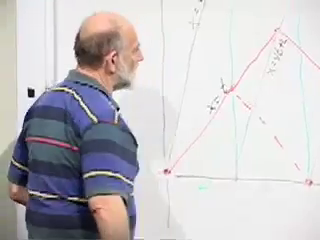
\includegraphics[width=0.72\textwidth]{lecture_01_figure_04.png}
\caption{Der vorwärts laufende Lichtstrahl \(x=t\) schneidet die mittlere Weltlinie des bewegten Gitters.}
\lectureframe{01:02:33}
\end{figure}

Die vollständige Geometrie lässt sich auch zeichnen, ohne dass eine Person an der Tafel im Weg steht:

\begin{figure}[H]
\centering
\begin{tikzpicture}[scale=0.95]
\draw[->] (-0.5,0) -- (6.5,0) node[right] {$x$};
\draw[->] (0,-0.2) -- (0,4.3) node[above] {$t$};
\draw[blue] (0,0) -- (1.4,4.0);
\draw[blue] (2.0,0) -- (3.4,4.0);
\draw[blue] (4.0,0) -- (5.4,4.0);
\draw[red] (0,0) -- (3.08,3.08);
\draw[red] (3.08,3.08) -- (4.56,1.60);
\draw[red,dashed] (2.0,0) -- (4.56,1.60);
\fill (0,0) circle (1.5pt);
\fill (2.0,0) circle (1.5pt);
\fill (4.0,0) circle (1.5pt);
\fill (3.08,3.08) circle (1.5pt);
\fill (4.56,1.60) circle (1.5pt);
\node[left] at (0.55,1.55) {$x=vt$};
\node[left] at (2.45,1.9) {$x=vt+L$};
\node[right] at (4.72,1.9) {$x=vt+2L$};
\node[left] at (1.88,2.28) {$x=t$};
\node[above right] at (3.08,3.08) {$A$};
\end{tikzpicture}
\caption{Lichtsignale bestimmen die Gleichzeitigkeitslinie des bewegten Bezugssystems.}
\end{figure}

Senden wir vom Ursprung einen nach rechts laufenden Lichtstrahl aus. Sei \(A\) sein Schnittpunkt mit der mittleren Weltlinie. Die beiden Gleichungen bei \(A\) lauten
\begin{align}
x&=t,\\
x&=vt+L.
\end{align}
Einsetzen ergibt
\begin{equation}
t=vt+L,
\end{equation}
und damit
\begin{equation}
t_A=x_A=\frac{L}{1-v}.
\label{eq:point-a}
\end{equation}

Von \(A\) aus verfolgen wir einen nach links laufenden Lichtstrahl rückwärts bis zur rechtesten bewegten Weltlinie. Seine Gleichung hat die Form
\begin{equation}
x+t=b.
\end{equation}
Da er durch \(A\) verläuft, legt Gleichung~\eqref{eq:point-a} die Konstante fest:
\begin{equation}
b=x_A+t_A=\frac{2L}{1-v}.
\end{equation}
Damit erfüllt der rückwärts laufende Strahl
\begin{equation}
x+t=\frac{2L}{1-v}.
\label{eq:backward-ray}
\end{equation}

Sein Schnittpunkt mit der rechtesten Weltlinie ergibt sich aus
\begin{align}
x+t&=\frac{2L}{1-v},\\
x&=vt+2L.
\end{align}
Eliminieren wir \(x\), so erhalten wir
\begin{align}
(1+v)t
  &=2L\left(\frac{1}{1-v}-1\right)\\
  &=\frac{2Lv}{1-v},
\end{align}
also
\begin{equation}
t=\frac{2Lv}{1-v^2}.
\end{equation}
Einsetzen in \(x=vt+2L\) ergibt
\begin{equation}
x=\frac{2L}{1-v^2}.
\end{equation}
Die Koordinaten selbst sind weniger wichtig als ihr Verhältnis:
\begin{equation}
\frac{t}{x}=v.
\end{equation}
Somit liegt jedes Ereignis, das den bewegten Uhren zufolge gleichzeitig mit dem Ursprung ist, auf
\begin{equation}
t=vx,
\label{eq:simultaneity-c-one}
\end{equation}
wohingegen der bewegte Ursprung der Linie
\begin{equation}
x=vt.
\label{eq:moving-time-axis}
\end{equation}
folgt. Die beiden Achsen sind symmetrisch um den Lichtstrahl bei \(45^\circ\) geneigt.

Alle Punkte auf \(x=vt\) haben dieselbe gestrichene Ortskoordinate \(x'=0\), während ihre gestrichenen Zeiten variieren. Alle Punkte auf \(t=vx\) haben dieselbe gestrichene Zeit \(t'=0\), während ihre gestrichenen Ortskoordinaten variieren. Die eine Linie ist somit die gestrichene Zeitachse, die andere die gestrichene Ortsachse. Die aufwendige Signalkonstruktion war nötig, um die zweite Linie zu bestimmen; aus der Weltlinie des bewegten Ursprungs allein ließ sie sich nicht ableiten.

Um in Gleichung~\eqref{eq:simultaneity-c-one} die gewöhnlichen Einheiten wieder einzusetzen, braucht man
\begin{equation}
t=\frac{v}{c^2}x.
\label{eq:simultaneity-dimensional}
\end{equation}
Der Faktor \(c^2\) erklärt, weshalb das Newtonsche Bild im Alltag so gut funktioniert. Für Geschwindigkeiten, die sehr klein gegenüber \(c\) sind, ist die Neigung der bewegten Gleichzeitigkeitslinie äußerst gering.

\begin{figure}[H]
\centering
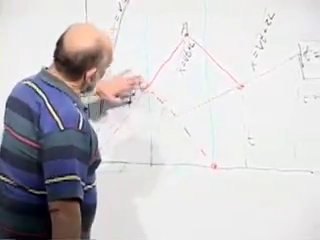
\includegraphics[width=0.72\textwidth]{lecture_01_figure_05.png}
\caption{Bei \(c=1\) sind die gestrichenen Zeit- und Gleichzeitigkeitsachsen symmetrisch zum Lichtstrahl.}
\lectureframe{01:15:40}
\end{figure}

\begin{figure}[H]
\centering
\begin{tikzpicture}[scale=1.0]
\draw[->] (-2.2,0) -- (5.2,0) node[right] {$x$};
\draw[->] (0,-0.2) -- (0,4.9) node[above] {$t$};
\draw[red] (0,0) -- (3.9,3.9);
\draw[red] (0,0) -- (-1.8,1.8);
\draw[blue] (0,0) -- (1.8,4.5);
\draw[blue,dashed] (0,0) -- (4.5,1.8);
\node[right] at (3.9,3.9) {$x=t$};
\node[left] at (-1.8,1.8) {$x=-t$};
\node[above] at (1.8,4.5) {$x'=0$};
\node[right] at (4.5,1.8) {$t'=0$};
\end{tikzpicture}
\caption{Die gestrichenen Achsen und invarianten Lichtstrahlen in Einheiten mit \(c=1\).}
\end{figure}

\section{Herleitung der Lorentz-Transformation}

Die Geometrie legt fest, wo jede gestrichene Koordinate verschwindet. Auf der bewegten Zeitachse \(x=vt\) muss \(x'=0\) gelten. Auf der bewegten Gleichzeitigkeitsachse \(t=vx\) muss \(t'=0\) gelten. Die allgemeinsten linearen Beziehungen mit diesen Nullstellen lassen sich schreiben als
\begin{align}
x'&=\frac{x-vt}{F(v)},\\
t'&=\frac{t-vx}{G(v)}.
\label{eq:fg-ansatz}
\end{align}
Die Faktoren \(F\) und \(G\) erlauben, dass sich die Skalen der gestrichenen Koordinaten von den Galileischen Skalen unterscheiden, obwohl die Achsen bereits festgelegt sind. Die Linearität folgt aus der Homogenität von Raum und Zeit: Eine Verschiebung des Experiments kann das Transformationsgesetz nicht ändern.\editorialnote{Dieses kurze Linearitätsargument macht eine Annahme explizit, die bei der Herleitung an der Tafel implizit verwendet wurde.}

Bis hierhin hat uns die Geometrie vieles, aber noch nicht alles mitgeteilt. Die Zähler legen die Neigung der Achsen fest. Sie bestimmen nicht den Einheitenabstand entlang dieser Achsen. Genau für diese noch fehlende Skalierungsinformation stehen \(F(v)\) und \(G(v)\).

Nun fordern wir die Invarianz der Lichtgeschwindigkeit. Ein nach rechts laufender Strahl, der \(x=t\) erfüllt, muss auch \(x'=t'\) erfüllen. Entlang dieses Strahls gilt
\begin{align}
x'&=\frac{(1-v)t}{F(v)},\\
t'&=\frac{(1-v)t}{G(v)}.
\end{align}
Die Gleichheit für jeden Punkt auf dem Strahl verlangt
\begin{equation}
F(v)=G(v).
\end{equation}
Wir können daher schreiben
\begin{align}
x'&=\frac{x-vt}{F(v)},\\
t'&=\frac{t-vx}{F(v)}.
\label{eq:common-f}
\end{align}

Dieser Schritt bringt die erste wirklich Einsteinische Forderung in die Algebra ein. Dieselbe geometrische Linie ist für beide Beobachter ein Lichtstrahl; daher müssen die beiden gestrichenen Koordinaten entlang dieser Linie gleich stark zunehmen, wenn \(c=1\). Unterschiedliche Faktoren in den beiden Gleichungen würden dazu führen, dass sich die gestrichene Geschwindigkeit von eins unterscheidet.

Eine unbekannte Funktion bleibt noch. Multiplizieren wir Gleichung~\eqref{eq:common-f} mit \(F(v)\):
\begin{align}
F(v)x'&=x-vt,\\
F(v)t'&=t-vx.
\end{align}
Multiplizieren wir die zweite Gleichung mit \(v\) und addieren sie zur ersten, fällt \(t\) heraus. Damit ergibt sich
\begin{equation}
(1-v^2)x=F(v)(x'+vt').
\end{equation}
Entsprechend folgt
\begin{equation}
(1-v^2)t=F(v)(t'+vx').
\end{equation}
Die inverse Transformation lautet somit
\begin{align}
x&=\frac{F(v)}{1-v^2}(x'+vt'),\\
t&=\frac{F(v)}{1-v^2}(t'+vx').
\end{align}

Das Relativitätsprinzip macht die beiden Bezugssysteme wechselseitig gleichberechtigt. Sieht der Bahnhof den Zug mit \(+v\) fahren, so sieht der Zug den Bahnhof mit \(-v\) fahren. Die inversen Gleichungen müssen deshalb dieselbe Form wie die Vorwärtstransformation haben, wobei das Vorzeichen von \(v\) umgekehrt ist. Die Vorfaktoren müssen also erfüllen:
\begin{equation}
\frac{F(v)}{1-v^2}=\frac{1}{F(v)}.
\end{equation}
Daraus folgt
\begin{equation}
F(v)^2=1-v^2,
\end{equation}
und die Stetigkeit mit der Identitätstransformation bei \(v=0\) wählt die positive Wurzel:
\begin{equation}
F(v)=\sqrt{1-v^2}.
\end{equation}

Es wurde nichts an einen bestimmten Lichtimpuls angepasst. Das Ergebnis folgt aus den durch Synchronisation festgelegten Achsen, der gemeinsamen Lichtgeschwindigkeit und der Forderung, dass keines der beiden Inertialsysteme gegenüber dem anderen ausgezeichnet sein darf.

Die Lorentz-Transformation in Einheiten mit \(c=1\) lautet
\begin{align}
x'&=\frac{x-vt}{\sqrt{1-v^2}},\\
t'&=\frac{t-vx}{\sqrt{1-v^2}}.
\label{eq:lorentz-c-one}
\end{align}
Ihre inverse Transformation ist
\begin{align}
x&=\frac{x'+vt'}{\sqrt{1-v^2}},\\
t&=\frac{t'+vx'}{\sqrt{1-v^2}}.
\end{align}

\begin{figure}[H]
\centering
\includegraphics[width=0.76\textwidth]{lecture_01_figure_06.png}
\caption{Die vollständige Lorentz-Transformation für \(c=1\) an der Tafel.}
\lectureframe{01:32:38}
\end{figure}

Die wesentliche Neuerung zeigt sich bereits in der Zeitgleichung. Die Zeit wird nicht einfach unverändert von einem Bezugssystem ins andere übertragen. Eine gestrichene Zeitkoordinate enthält sowohl ungestrichene Zeit als auch den ungestrichenen Ort. Folglich beschreiben \(t=\text{constant}\) und \(t'=\text{constant}\) unterschiedliche Ereignismengen.

Der Mischungsterm ist keine optionale, nachträglich angefügte Korrektur. Ohne ihn bliebe die Linie \(t'=0\) horizontal, die Gleichzeitigkeit entfernter Ereignisse wäre weiterhin universell, und die Transformation könnte die Lichtgeschwindigkeit nicht erhalten.

\section{Lichtgeschwindigkeit wieder einsetzen und das Ergebnis überprüfen}

Für \(c\ne1\) stellt die Dimensionskonsistenz die fehlenden Faktoren wieder her. Das Verhältnis \(v^2/c^2\) ist dimensionslos, während \((v/c^2)x\) die Dimension einer Zeit hat. Somit gilt
\begin{align}
x'&=\frac{x-vt}{\sqrt{1-v^2/c^2}},\\
t'&=\frac{t-(v/c^2)x}{\sqrt{1-v^2/c^2}}.
\label{eq:lorentz-dimensional}
\end{align}
Die inverse Transformation erhält man, indem man das Vorzeichen von \(v\) umkehrt:
\begin{align}
x&=\frac{x'+vt'}{\sqrt{1-v^2/c^2}},\\
t&=\frac{t'+(v/c^2)x'}{\sqrt{1-v^2/c^2}}.
\end{align}
Die Einführung von
\begin{equation}
\gamma=\frac{1}{\sqrt{1-v^2/c^2}}
\end{equation}
würde die vertraute kompakte Form ergeben; die Schreibweise mit dem Nenner macht jedoch die Herleitung besser nachvollziehbar.

Numerisch ist \(c\simeq3\times10^8\,\mathrm{m/s}\), also \(c^2\simeq9\times10^{16}\,\mathrm{m^2/s^2}\). Der große Nenner macht sowohl die Neigung der Gleichzeitigkeitslinie als auch den Faktor \(v^2/c^2\) bei den meisten mechanischen Experimenten unmerklich. Diese geringe Größe erklärt Galileis Erfolg; sie stellt die absolute Zeit nicht wieder her.

\begin{figure}[H]
\centering
\includegraphics[width=0.76\textwidth]{lecture_01_figure_07.png}
\caption{Die Lorentz-Transformation mit wieder eingesetzten Faktoren von \(c\).}
\lectureframe{01:35:58}
\end{figure}

Zwei Überprüfungen liegen unmittelbar nahe. Betrachten wir zunächst \(v\ll c\). Dann ist \(v^2/c^2\) vernachlässigbar, und bei gewöhnlichen Entfernungen ist auch der Term der Relativität der Gleichzeitigkeit \(vx/c^2\) vernachlässigbar. Gleichung~\eqref{eq:lorentz-dimensional} vereinfacht sich zu
\begin{equation}
t'\approx t,\qquad x'\approx x-vt.
\end{equation}
Die Galilei-Relativität ergibt sich als Näherung für niedrige Geschwindigkeiten.

Prüfen wir zweitens einen Lichtstrahl. Nachdem \(c\) wieder eingesetzt wurde, erfüllt ein nach rechts laufender Strahl \(x=ct\), nicht \(x=t\). Einsetzen ergibt
\begin{align}
x'&=\frac{(c-v)t}{\sqrt{1-v^2/c^2}},\\
t'&=\frac{(1-v/c)t}{\sqrt{1-v^2/c^2}}.
\end{align}
Da \(c-v=c(1-v/c)\) gilt,
\begin{equation}
x'=ct'.
\end{equation}
misst der gestrichene Beobachter dieselbe Geschwindigkeit \(c\). Für einen nach links laufenden Strahl ergibt das Einsetzen von \(x=-ct\) entsprechend
\begin{equation}
x'=-ct'.
\end{equation}
Die Transformation behandelt Licht, das sich in beide Richtungen ausbreitet, korrekt.

Die Unterscheidung zwischen \(x=t\) und \(x=ct\) ist eine lehrreiche Dimensionsprüfung. Der erstere Ausdruck ist nur in Einheiten korrekt, in denen \(c=1\) gilt. Würde man in der Transformation die gewöhnlichen Einheiten wieder einsetzen, die Strahlgleichung aber in natürlichen Einheiten belassen, vermischte man zwei Konventionen und erhielte ein falsches Ergebnis. Die Dimensionskonsistenz deckt den Fehler sofort auf.

\section{Das Mittelpunktkriterium}

\begin{classroomqa}
\audiencequestion{Angenommen, ein Beobachter empfängt zwei Lichtblitze gleichzeitig, befindet sich aber nicht auf halbem Weg zwischen ihren Quellen. Kann dieser Beobachter daraus schließen, dass die Blitze gleichzeitig ausgesendet wurden?
\lecturetimestamp{01:42:55}}
\lecturerresponse{Nein. Gleiche Ankunftszeiten bedeuten nur für den Beobachter gleiche Aussendezeiten, der sich im betreffenden Bezugssystem räumlich genau zwischen den beiden Quellen befindet. Ein Empfänger, der einer Quelle näher ist, kann beide Blitze gleichzeitig empfangen, obwohl der weiter entfernte Blitz früher ausgesendet wurde. In der bewegten Konstruktion ist die Weltlinie des Mittelpunkts \(x=vt+L\) daher wesentlich. Dem Vorwärtsstrahl \(x=t\) folgt man, bis er diesen Mittelpunkt erreicht, und anschließend verfolgt man einen rückwärts laufenden Lichtstrahl bis \(x=vt+2L\). Dieses zweite Endereignis ist nach dem bewegten Bezugssystem gleichzeitig mit dem Ursprung, nicht etwa ein beliebiges Ereignis an einem anderen Ort mit gleicher Ankunftszeit.}
\end{classroomqa}

Wir haben die vollständige Koordinatentransformation erreicht, aber noch nicht ihre bekanntesten Folgerungen. Als Nächstes folgen die Längenkontraktion, die Zeitdilatation und die Eigenzeit, danach relativistischer Impuls und relativistische Energie. Die Grundlage ist bereits gelegt: Jedes Inertialsystem kann dieselben Gesetze verwenden und dieselbe Lichtgeschwindigkeit messen, weil sich Raum und Zeit miteinander vermischen und weil die Gleichzeitigkeit entfernter Ereignisse zu einem Bezugssystem gehört und nicht absolut zur Welt.
\chapter{Maxwell-Gleichungen, Kovarianz und elektromagnetische Wellen}

\lectureoverview{Elektrische und magnetische Felder üben über die Lorentzkraft Kräfte auf geladene Materie aus, doch Materie muss auch die Felder erzeugen und umverteilen. Wir formulieren diese wechselseitige Seite des Elektromagnetismus, zeigen, dass die Maxwell-Gleichungen Lorentz-kovariant sind, leiten ihre Well Lösungen her und führen anschließend Ladung und Strom in einer Form wieder ein, in der die lokale Erhaltung unmittelbar sichtbar ist. In der gesamten Vorlesung verwenden wir Einheiten, in denen \(c=1\) gilt.}

\section{Die andere Seite des Elektromagnetismus}

Beginnen wir mit dem Teil des Themas, den wir bereits behandelt haben. Bewegt sich ein Teilchen mit der Ladung \(q\) und der Geschwindigkeit \(\mathbf v\) durch elektrische und magnetische Felder, so wirkt auf es die Kraft
\begin{equation}
\mathbf F=q\bigl(\mathbf E+\mathbf v\times\mathbf B\bigr).
\label{eq:lorentz-force-three}
\end{equation}
Der Faktor \(q\) ist unverzichtbar. Ein ungeladenes Teilchen erfährt keine elektromagnetische Kraft. Der elektrische Beitrag wirkt auch dann, wenn das Teilchen momentan in Ruhe ist, während der magnetische Beitrag von seiner Bewegung abhängt.

Gleichung~\eqref{eq:lorentz-force-three} sagt uns, wie vorgegebene Felder auf Materie wirken. Sie sagt uns nicht, wodurch die Felder bestimmt werden. Was erzeugt ein elektrisches Feld um einen Gegenstand, ein magnetisches Feld um einen anderen oder eine Welle, die sich durch den leeren Raum bewegt? Die Gleichungen, die diese Fragen beantworten, sind die Maxwell-Gleichungen.

\begin{figure}[H]
\centering
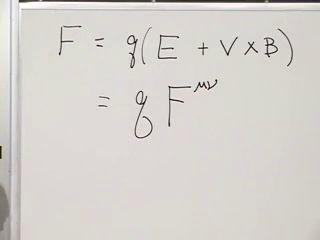
\includegraphics[width=0.62\textwidth]{lecture_58_figure_02.png}
\caption{Die Lorentzkraft als Dreivektorgleichung und der Beginn ihrer tensorielle Umformulierung.}
\lectureframe{00:05:49}
\end{figure}

Die relativistische Form des Kraftgesetzes führt die Notation ein, die wir benötigen werden:
\begin{equation}
f^\mu=qF^\mu{}_{\nu}u^\nu.
\label{eq:lorentz-force-four}
\end{equation}
Hier ist \(u^\nu\) die Vierergeschwindigkeit, \(f^\mu\) die Viererkraft und \(F^{\mu\nu}\) ein antisymmetrischer Tensor, der aus \(\mathbf E\) und \(\mathbf B\) zusammengesetzt ist. Auf der Tafel ist zunächst nur der schematische Anfang dieses Ausdrucks zu sehen; die Kontraktion mit \(u^\nu\) liefert den fehlenden Vektor, sodass ein Kraftindex frei bleibt.

Es gibt einen physikalischen Grund dafür, dass Materie auf das Feld zurückwirken muss. Eine elektromagnetische Welle kann auf eine Ladung treffen, sie beschleunigen und ihr Energie übertragen. Könnte das Feld auf die Ladung einwirken, während die Ladung niemals auf das Feld einwirken könnte, gäbe es keinen Ort, von dem diese Energie entzogen würde. Wirkung und Gegenwirkung sind nicht das ganze Argument, aber die Energieerhaltung macht die wechselseitige Kopplung unvermeidlich.

\section{Eine sich ändernde Quelle sendet eine Störung aus}

Eine Punktladung erzeugt ein elektrisches Feld, das von ihrem Ort nach außen oder nach innen gerichtet ist. Ein Strom in einem Draht--ein Fluss geladener Teilchen--erzeugt ein Magnetfeld, das den Draht umkreist. Diese vertrauten statischen Bilder zeigen bereits zwei unterschiedliche geometrische Muster: Der elektrische Fluss geht von Ladung aus, während sich die magnetischen Feldlinien um den Strom winden.

Bewegen wir nun die Punktladung plötzlich. In der Nähe ihrer neuen Position muss sich das elektrische Feld neu ordnen, doch ein weit entfernter Beobachter kann nicht augenblicklich von der Bewegung erfahren. In großer Entfernung bleibt das alte Feld bestehen, bis ein Signal Zeit hatte, dort anzukommen. Zwischen dem nahen und dem fernen Bereich liegt eine sich bewegende Front, an der sich das Feld ändert. Diese sich ausbreitende Neuordnung ist eine elektromagnetische Störung.

Wird die Ladung hin und her bewegt, folgen die Neuordnungen aufeinander und bilden eine elektromagnetische Welle. Dies ist die grundlegende Funktion einer Antenne: Ein oszillierender elektrischer Strom sendet eine Feldstörung nach außen. Eine Umkehr des Stroms in einem Draht liefert dasselbe Argument für das Magnetfeld. Die Umlaufrichtung von \(\mathbf B\) muss sich umkehren, doch die Umkehr breitet sich aus, statt überall zugleich aufzutreten.

Dieses Kausalbild gibt den Maxwell-Gleichungen zwei Ziele vor. Sie müssen beschreiben, wie Ladung und Strom die Felder hervorrufen, und sie müssen zulassen, dass sich Änderungen dieser Felder höchstens mit Lichtgeschwindigkeit ausbreiten. Das zweite Ziel ist zugleich eine Prüfung der Relativitätstheorie. Haben die Maxwell-Gleichungen in jedem Inertialsystem dieselbe Form und ergeben sie eine bestimmte Wellengeschwindigkeit, dann muss jedes Inertialsystem aus ihnen dieselbe Geschwindigkeit folgern.

\section{Rückblick auf die relativistische Wellengleichung}

Betrachten wir vor den Vektorfeldern ein Skalarfeld \(\phi(\mathbf x,t)\), also eine Zahl an jedem Punkt der Raumzeit. Eine Gleichung mit einer Ableitung
\begin{equation}
\partial_\mu\phi=0
\end{equation}
würde besagen, dass alle Raumzeit-Ableitungen verschwinden. Das Feld wäre konstant und könnte daher keine Welle tragen. Eine nichttriviale relativistische Wellengleichung enthält zwei Ableitungen:
\begin{equation}
\partial_\mu\partial^\mu\phi=0.
\end{equation}
Mit der hier verwendeten Vorzeichenkonvention gilt
\begin{equation}
\left(\partial_t^2-\partial_x^2-\partial_y^2-\partial_z^2\right)\phi=0,
\label{eq:scalar-wave-four}
\end{equation}
oder kürzer
\begin{equation}
\left(\partial_t^2-\nabla^2\right)\phi=0.
\end{equation}
Die Wahl \(c=1\) sorgt dafür, dass Zeit und Entfernung Einheiten haben, die zueinander passen. Stellt man die üblichen Einheiten wieder her, steht neben der zweiten Zeitableitung der Faktor \(1/c^2\).

Für eine Welle, die sich entlang der \(z\)-Achse ausbreitet, hängt das Feld von \(z\) und \(t\) ab, nicht von \(x\) oder \(y\). Gleichung~\eqref{eq:scalar-wave-four} vereinfacht sich zu
\begin{equation}
\left(\partial_t^2-\partial_z^2\right)\phi=0.
\label{eq:scalar-wave-one}
\end{equation}

\begin{figure}[H]
\centering
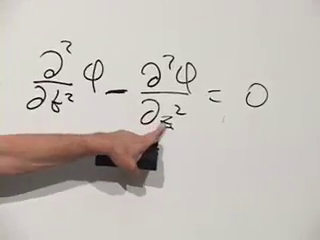
\includegraphics[width=0.56\textwidth]{lecture_58_figure_04.png}
\caption{Die eindimensionale skalare Wellengleichung als Modell für elektromagnetische Wellen.}
\lectureframe{00:47:03}
\end{figure}

Ihre allgemeine Form als Summe laufender Wellen lautet
\begin{equation}
\phi(z,t)=f(z-t)+g(z+t).
\end{equation}
Das Profil \(f(z-t)\) bewegt sich in Richtung zunehmender Werte von \(z\), denn ein Punkt konstanter Phase erfüllt \(z-t=\text{constant}\). Das Profil \(g(z+t)\) bewegt sich in die entgegengesetzte Richtung. Keines der Profile muss sinusförmig sein; jede hinreichend glatte Form verschiebt sich, ohne ihre Gestalt zu ändern.

Sinusfunktionen sind dennoch praktisch:
\begin{equation}
\phi(z,t)=A\cos\!\bigl(k(z-t)\bigr).
\end{equation}
Die Wellenzahl \(k\) bestimmt die Wellenlänge:
\begin{equation}
\lambda=\frac{2\pi}{k}.
\end{equation}
Ein großer Wert von \(k\) führt zu schnellen räumlichen Oszillationen und einer kurzen Wellenlänge; ein kleiner Wert von \(k\) führt zu einer langen Wellenlänge. Dieselben Profile werden bald zu Komponenten von \(\mathbf E\) und \(\mathbf B\).

\section{Die Vektorrechnung, die Maxwell braucht}

Die Maxwell-Gleichungen sind mit Skalarprodukten, Kreuzprodukten, Divergenz und Rotation formuliert. Es lohnt sich, die Notation einmal neu aufzubauen, denn bei den späteren Komponentenrechnungen verwenden wir genau diese Muster.

Für gewöhnliche Dreivektoren \(\mathbf a\) und \(\mathbf b\) ist das Skalarprodukt der Skalar
\begin{equation}
\mathbf a\cdot\mathbf b
=a_xb_x+a_yb_y+a_zb_z.
\end{equation}
Das Kreuzprodukt ist ein weiterer Vektor:
\begin{align}
(\mathbf a\times\mathbf b)_x&=a_yb_z-a_zb_y,\\
(\mathbf a\times\mathbf b)_y&=a_zb_x-a_xb_z,\\
(\mathbf a\times\mathbf b)_z&=a_xb_y-a_yb_x.
\end{align}
Die übrigen Komponenten ergeben sich aus der zyklischen Reihenfolge \(x\to y\to z\to x\).

Führen wir den Differentialoperator ein:
\begin{equation}
\boldsymbol\nabla=
\left(\partial_x,\partial_y,\partial_z\right).
\end{equation}
Seine Einträge sind Operatoren und keine gewöhnlichen Zahlen, doch die Muster für Skalar- und Kreuzprodukte lassen sich weiterhin verwenden. Für ein Vektorfeld \(\mathbf A\) ist
\begin{equation}
\boldsymbol\nabla\cdot\mathbf A
=\partial_xA_x+\partial_yA_y+\partial_zA_z
\label{eq:divergence}
\end{equation}
die Divergenz, während
\begin{align}
(\boldsymbol\nabla\times\mathbf A)_x
 &=\partial_yA_z-\partial_zA_y,\\
(\boldsymbol\nabla\times\mathbf A)_y
 &=\partial_zA_x-\partial_xA_z,\\
(\boldsymbol\nabla\times\mathbf A)_z
 &=\partial_xA_y-\partial_yA_x
\label{eq:curl}
\end{align}
die Komponenten der Rotation sind.

Die Geometrie ist ebenso wichtig wie die Formeln. Ein Vektorfeld hat dort eine positive Divergenz, wo es so aussieht, als ströme es von einer Quelle nach außen. Es hat dort eine Rotation, wo es umläuft. Das radiale elektrische Feld einer Punktladung veranschaulicht die Divergenz; das Magnetfeld, das sich um einen stromdurchflossenen Draht windet, veranschaulicht die Rotation. Ein räumlich konstantes Vektorfeld hat weder das eine noch das andere.

\section{Die Maxwell-Gleichungen im Vakuum}

In Abwesenheit von Ladung und Strom lauten die Maxwell-Gleichungen
\begin{align}
\boldsymbol\nabla\times\mathbf E&=-\partial_t\mathbf B,
\label{eq:faraday-vac}\\
\boldsymbol\nabla\cdot\mathbf B&=0,
\label{eq:gauss-b-vac}\\
\boldsymbol\nabla\times\mathbf B&=\partial_t\mathbf E,
\label{eq:ampere-vac}\\
\boldsymbol\nabla\cdot\mathbf E&=0.
\label{eq:gauss-e-vac}
\end{align}
Die beiden Rotationsgleichungen gehen nahezu ineinander über, wenn man \(\mathbf E\) und \(\mathbf B\) vertauscht; ein wesentliches Minuszeichen unterscheidet sie jedoch. Die beiden Divergenzgleichungen besagen, dass keines der Felder in dem betrachteten Vakuumbereich eine Quelle hat. Die Divergenz des Magnetfelds bleibt auch dann null, wenn elektrische Quellen wieder berücksichtigt werden; im gewöhnlichen Elektromagnetismus gibt es keine magnetische Ladung.

\begin{figure}[H]
\centering
\includegraphics[width=0.76\textwidth]{lecture_58_figure_06.png}
\caption{Die vier Maxwell-Gleichungen im Vakuum, so angeordnet, dass die weitgehende Symmetrie zwischen elektrischen und magnetischen Feldern sichtbar wird.}
\lectureframe{00:27:30}
\end{figure}

Die Ladungsdichte \(\rho\) wird später die Null auf der rechten Seite von Gleichung~\eqref{eq:gauss-e-vac} ersetzen, und die Stromdichte \(\mathbf J\) wird in Gleichung~\eqref{eq:ampere-vac} eingehen. Diese Terme lassen wir vorerst weg. Die quellenfreien Gleichungen zeigen die Transformationsstruktur und den Wellenmechanismus mit möglichst wenigen zusätzlichen Termen.

Sie schärfen auch Einsteins Rätsel. Ein Galilei-Beobachter, der einer Welle folgt, würde erwarten, Geschwindigkeiten voneinander abzuziehen und eine kleinere Wellengeschwindigkeit zu messen. Wenn jedoch dieselben Maxwell-Gleichungen in jedem Inertialsystem gelten, leitet jeder Beobachter daraus dieselbe Wellengeschwindigkeit von eins ab. Die Lösung besteht nicht darin, die Wellengleichung von einem Bezugssystem zum anderen abzuändern. Sie besteht darin, die Lorentz-Transformation zu verwenden und die Maxwell-Gleichungen in Größen darzustellen, deren Transformationsgesetze bereits bekannt sind.

\section{Elektrische und magnetische Felder als ein Tensor}

Die elektrischen und magnetischen Felder werden im antisymmetrischen Feldtensor zusammengefasst:
\begin{equation}
F^{\mu\nu}=
\begin{pmatrix}
0   & -E_x & -E_y & -E_z\\
E_x & 0    & -B_z & B_y\\
E_y & B_z  & 0    & -B_x\\
E_z & -B_y & B_x  & 0
\end{pmatrix},
\label{eq:l0203-field-tensor}
\end{equation}
wobei die Reihenfolge von Zeilen und Spalten \(t,x,y,z\) ist. Die Antisymmetrie
\begin{equation}
F^{\mu\nu}=-F^{\nu\mu},
\end{equation}
erzwingt, dass die Diagonaleinträge verschwinden, und bestimmt die untere Hälfte der Matrix durch die obere Hälfte. Die Raum-Zeit-Einträge enthalten \(\mathbf E\); die rein räumlichen Einträge enthalten \(\mathbf B\).

\begin{figure}[H]
\centering
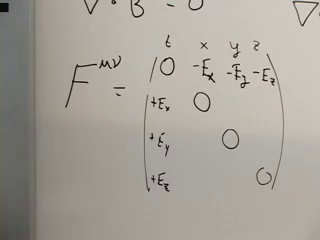
\includegraphics[width=0.58\textwidth]{lecture_58_figure_03.png}
\caption{Der vervollständigte elektromagnetische Feldtensor mit seinen elektrischen und magnetischen Einträgen.}
\lectureframe{00:32:05}
\end{figure}

Die Bedeutung von \(F^{\mu\nu}\) liegt nicht bloß darin, dass sich sechs Feldkomponenten in einer Matrix unterbringen lassen. Unter einer Lorentz-Transformation transformiert er sich wie ein Tensor zweiter Stufe. Von verschiedenen Beobachtern gemessene elektrische und magnetische Felder mischen sich daher genau so, wie es nötig ist, damit sich das gesamte Objekt konsistent transformiert.

Es gibt einen zweiten antisymmetrischen Tensor, den dualen Feldtensor \(\widetilde F^{\mu\nu}\). Gemäß der hier verwendeten Konvention erhält man ihn aus Gleichung~\eqref{eq:l0203-field-tensor} durch die Ersetzung
\begin{equation}
\mathbf E\longmapsto-\mathbf B,
\qquad
\mathbf B\longmapsto\mathbf E.
\label{eq:dual-replacement}
\end{equation}
Damit gilt
\begin{equation}
\widetilde F^{\mu\nu}=
\begin{pmatrix}
0    & B_x  & B_y  & B_z\\
-B_x & 0    & -E_z & E_y\\
-B_y & E_z  & 0    & -E_x\\
-B_z & -E_y & E_x  & 0
\end{pmatrix}.
\label{eq:dual-tensor}
\end{equation}
Das Vorzeichen in Gleichung~\eqref{eq:dual-replacement} ist wichtig. In der Vorlesung wird zunächst ein mündlicher Austausch versucht, dann die Abweichung beim Vorzeichen bemerkt und korrigiert, bevor die Matrix vervollständigt wird.

\begin{figure}[H]
\centering
\includegraphics[width=0.58\textwidth]{lecture_58_figure_07.png}
\caption{Der duale Tensor entsteht durch den Austausch der elektrischen und magnetischen Einträge mit dem erforderlichen Vorzeichen.}
\lectureframe{00:35:45}
\end{figure}

\section{Die kovarianten Gleichungen im Vakuum}

Jede Maxwell-Gleichung enthält eine Ableitung. Verknüpft man einen Rang-zwei-Tensor mit einer Ableitung, bleibt ein Index frei. Die natürlichen kovarianten Gleichungen sind daher
\begin{align}
\partial_\mu F^{\mu\nu}&=0,
\label{eq:maxwell-covariant-vac}\\
\partial_\mu\widetilde F^{\mu\nu}&=0.
\label{eq:maxwell-dual-vac}
\end{align}
Für jeden festen Wert von \(\nu\) ist Gleichung~\eqref{eq:maxwell-covariant-vac} eine Gleichung. Da \(\nu\) die Werte \(t,x,y,z\) annehmen kann, umfasst sie vier skalare Gleichungen. Gleichung~\eqref{eq:maxwell-dual-vac} umfasst die übrigen vier. Das entspricht den beiden Vektor-Rotationsgleichungen und den beiden skalaren Divergenzgleichungen der ursprünglichen Liste.

Die Kurzschreibweise ist nur dann nützlich, wenn sie die vertrauten Gleichungen wiedergibt. Setzen wir \(\nu=z\):
\begin{align}
\partial_\mu F^{\mu z}
&=\partial_tF^{tz}
  +\partial_xF^{xz}
  +\partial_yF^{yz}
  +\partial_zF^{zz}\\
&=-\partial_tE_z+\partial_xB_y-\partial_yB_x\\
&=-\partial_tE_z+
  \bigl(\boldsymbol\nabla\times\mathbf B\bigr)_z.
\end{align}
Der Term \(F^{zz}\) verschwindet aufgrund der Antisymmetrie. Setzt man den Ausdruck gleich null, erhält man die \(z\)-Komponente von
\begin{equation}
\boldsymbol\nabla\times\mathbf B=\partial_t\mathbf E.
\end{equation}
Die \(x\)- und \(y\)-Komponenten ergeben sich durch zyklisches Vertauschen der Indizes.

\begin{figure}[H]
\centering
\includegraphics[width=0.76\textwidth]{lecture_58_figure_08.png}
\caption{Komponentenweise Entwicklung der kovarianten Feldgleichung: Der diagonale Tensoreintrag verschwindet, und die übrigen Terme ergeben wieder die Maxwell-Gleichungen.}
\lectureframe{00:43:30}
\end{figure}

Betrachten wir nun die Zeitkomponente:
\begin{align}
\partial_\mu F^{\mu t}
&=\partial_tF^{tt}
  +\partial_xF^{xt}
  +\partial_yF^{yt}
  +\partial_zF^{zt}\\
&=\partial_xE_x+\partial_yE_y+\partial_zE_z\\
&=\boldsymbol\nabla\cdot\mathbf E.
\end{align}
Damit ergibt sich Gleichung~\eqref{eq:gauss-e-vac}. Dieselben Überprüfungen für den dualen Tensor liefern
\(\boldsymbol\nabla\cdot\mathbf B=0\) und
\(\boldsymbol\nabla\times\mathbf E=-\partial_t\mathbf B\).

Damit sind die kompakten Gleichungen hergeleitet und nicht bloß vermutet. Ihre Struktur mit einem freien Index zeigt, dass es Vierergleichungen sind; eine Lorentz-Transformation ändert also ihre Komponenten, aber nicht ihre Form. Das ist die präzise Bedeutung der Aussage, dass die Maxwell-Gleichungen im Vakuum in jedem Inertialsystem dieselben sind.

\section{Von Gleichungen erster Ordnung zur Welle}

Die Maxwell-Gleichungen enthalten nur Ableitungen erster Ordnung, während eine Wellengleichung Ableitungen zweiter Ordnung enthält. Der scheinbare Widerspruch löst sich dadurch auf, dass die Maxwell-Theorie zwei Felder miteinander koppelt. Ein Paar von Gleichungen erster Ordnung für \(\mathbf E\) und \(\mathbf B\) lässt sich zu einer Gleichung zweiter Ordnung für jeweils eines der beiden Felder allein zusammenfassen.

Leiten wir Gleichung~\eqref{eq:ampere-vac} nach der Zeit ab:
\begin{equation}
\partial_t^2\mathbf E
=\boldsymbol\nabla\times\partial_t\mathbf B.
\end{equation}
Das Faraday-Gesetz liefert die Zeitableitung von \(\mathbf B\):
\begin{equation}
\partial_t\mathbf B=-\boldsymbol\nabla\times\mathbf E,
\end{equation}
und damit
\begin{equation}
\partial_t^2\mathbf E
=-\boldsymbol\nabla\times
  \bigl(\boldsymbol\nabla\times\mathbf E\bigr).
\label{eq:double-curl}
\end{equation}

Auf der Tafel wird eine Komponente durchgerechnet, statt eine auswendig gelernte Identität zu verwenden. Für die \(x\)-Komponente gilt
\begin{align}
\bigl[\boldsymbol\nabla\times
(\boldsymbol\nabla\times\mathbf E)\bigr]_x
&=\partial_y(\boldsymbol\nabla\times\mathbf E)_z
 -\partial_z(\boldsymbol\nabla\times\mathbf E)_y\\
&=\partial_y(\partial_xE_y-\partial_yE_x)\\
&\quad-\partial_z(\partial_zE_x-\partial_xE_z)\\
&=\partial_x(\partial_yE_y+\partial_zE_z)
 -\partial_y^2E_x\\
&\quad-\partial_z^2E_x.
\end{align}
Addieren und subtrahieren wir \(\partial_x^2E_x\), um die Divergenz sichtbar zu machen:
\begin{align}
\bigl[\boldsymbol\nabla\times
(\boldsymbol\nabla\times\mathbf E)\bigr]_x
&=\partial_x(\boldsymbol\nabla\cdot\mathbf E)
 -\nabla^2E_x.
\label{eq:double-curl-x}
\end{align}
Im Vakuum gilt \(\boldsymbol\nabla\cdot\mathbf E=0\). Aus den Gleichungen~\eqref{eq:double-curl} und \eqref{eq:double-curl-x} folgt
\begin{equation}
\left(\partial_t^2-\nabla^2\right)E_x=0.
\label{eq:ex-wave}
\end{equation}

\begin{figure}[H]
\centering
\includegraphics[width=0.72\textwidth]{lecture_58_figure_09.png}
\caption{Die Komponentenrechnung führt zur Wellengleichung für \(E_x\).}
\lectureframe{00:57:10}
\end{figure}

Dieselbe Rechnung gilt für \(E_y\) und \(E_z\); eine analoge Elimination ergibt
\begin{equation}
\left(\partial_t^2-\nabla^2\right)\mathbf B=0.
\end{equation}
Elektrische und magnetische Felder können sich folglich als Wellen durch den leeren Raum ausbreiten. In den hier verwendeten Einheiten beträgt ihre Geschwindigkeit eins; stellt man die üblichen Einheiten wieder her, ist sie gleich \(c\).

\section{Eine ebene Welle und ihre Polarisation}

Konstruieren wir eine einfache Welle, die sich in positiver \(z\)-Richtung ausbreitet:
\begin{equation}
\mathbf E(z,t)
=\widehat{\mathbf x}\,E_0
  \cos\!\bigl(k(z-t)\bigr).
\label{eq:plane-e}
\end{equation}
Ihr Profil bewegt sich entlang \(z\), ohne seine Form zu ändern. Da das elektrische Feld entlang der \(x\)-Achse zeigt, ist die Welle in \(x\)-Richtung linear polarisiert. Wir haben \(E_y=0\) gewählt, um das Beispiel einfach zu halten; eine zweite transversale Polarisation ließe sich ergänzen.

Die longitudinale Komponente ist nicht ebenso frei. Da die Welle nur von \(z\) und \(t\) abhängt, gilt
\begin{equation}
\boldsymbol\nabla\cdot\mathbf E
=\partial_zE_z=0.
\end{equation}
Somit kann \(E_z\) konstant sein, aber nicht das veränderliche Wellenprofil enthalten. Ein homogenes Hintergrundfeld kann unabhängig davon überlagert oder entfernt werden; es gehört nicht zur sich ausbreitenden Strahlung. Die Welle selbst ist transversal:
\begin{equation}
\mathbf E_{\mathrm{wave}}\cdot\widehat{\mathbf z}=0.
\end{equation}

Das Faraday-Gesetz legt das Magnetfeld fest. Für Gleichung~\eqref{eq:plane-e} ist die einzige von null verschiedene Komponente von \(\boldsymbol\nabla\times\mathbf E\) die \(y\)-Komponente:
\begin{equation}
(\boldsymbol\nabla\times\mathbf E)_y=\partial_zE_x.
\end{equation}
Folglich zeigt \(\partial_t\mathbf B\) in Richtung \(y\), und eine dazu passende Wahl ist
\begin{equation}
\mathbf B(z,t)
=\widehat{\mathbf y}\,E_0
  \cos\!\bigl(k(z-t)\bigr).
\label{eq:plane-b}
\end{equation}
In diesen Einheiten sind die Amplituden der elektrischen und magnetischen Felder gleich. Ihre Orientierung erfüllt
\begin{equation}
\mathbf E\perp\mathbf B,
\qquad
\mathbf E\perp\widehat{\mathbf z},
\qquad
\mathbf B\perp\widehat{\mathbf z},
\qquad
\mathbf E\times\mathbf B\parallel\widehat{\mathbf z}.
\end{equation}

\begin{figure}[H]
\centering
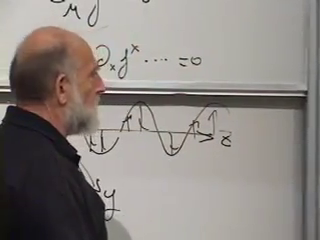
\includegraphics[width=0.70\textwidth]{lecture_58_figure_05.png}
\caption{Die fertige Skizze der transversalen elektromagnetischen Welle auf der Tafel: Die elektrischen und magnetischen Oszillationen stehen senkrecht zueinander und zur Ausbreitungsrichtung.}
\lectureframe{01:05:25}
\end{figure}

\begin{figure}[H]
\centering
\scalebox{0.90}{%
\begin{tikzpicture}[x=1cm,y=1cm,>=Latex]
  \draw[->,thick] (0,0) -- (8.2,0) node[right] {$z$};
  \draw[->,thick] (0,-1.6) -- (0,1.7) node[above] {$x$};
  \draw[->,thick] (0,0) -- (-1.15,-0.8) node[below left] {$y$};
  \draw[blue!70!black,thick,domain=0:7.5,samples=120]
    plot (\x,{0.95*sin(90*\x)});
  \foreach \z/\s in {0.8/1,2.8/-1,4.8/1,6.8/-1}{
    \draw[->,green!45!black,thick]
      (\z,0) -- ++({-0.55*\s},{-0.38*\s});
  }
  \node[blue!70!black] at (6.9,1.25) {$\mathbf E$};
  \node[green!45!black] at (5.2,-1.05) {$\mathbf B$};
  \draw[->,very thick] (6.2,1.55) -- (7.7,1.55)
    node[midway,above] {propagation};
\end{tikzpicture}
}
\caption{Die Felder \(\mathbf E\) und \(\mathbf B\) stehen senkrecht zueinander und zur Ausbreitungsrichtung.}
\end{figure}

Das ist die typische Eigenschaft des Lichts und aller elektromagnetischen Strahlung im Vakuum. Da die Gleichungen, aus denen die Welle folgt, Lorentz-kovariant sind, beschreibt auch ein anderer Inertialbeobachter eine elektromagnetische Welle, die sich mit \(c\) ausbreitet und transversale elektrische und magnetische Felder besitzt.

\section{Ladungsdichte und Stromdichte}

Nun führen wir die Quellen wieder ein, die wir vorübergehend beiseitegelassen haben. Befinden sich viele geladene Teilchen in einem Gebiet, ist es nützlich, sie durch Mittelung zu einer kontinuierlichen Ladungsdichte zusammenzufassen:
\begin{equation}
\rho(\mathbf x,t)=\frac{dQ}{dV}.
\end{equation}
Diese Näherung ähnelt der Beschreibung von Wasser als kontinuierlicher Flüssigkeit, obwohl es aus Molekülen besteht. Positive und negative Ladungen gehen mit entgegengesetzten Vorzeichen ein, sodass \(\rho\) die Nettoladung pro Volumeneinheit ist.

Die Ladung in einem gewählten Gebiet \(V\) beträgt
\begin{equation}
Q_V(t)=\int_V\rho(\mathbf x,t)\,dV.
\label{eq:charge-volume}
\end{equation}
Die Dichte kann von Ort und Zeit abhängen. Eine Ansammlung von Ladung kann sich von einem Punkt entfernen und dort die lokale Dichte ändern. Sie kann sich jedoch nicht beliebig ändern. Die Natur erhält die elektrische Ladung.

Die globale Erhaltung allein wäre zu schwach. Sie würde zulassen, dass Ladung auf der Erde verschwindet und im selben Augenblick auf dem Mars wieder auftaucht, solange die Gesamtladung unverändert bliebe. Die stärkere Aussage gilt lokal: Ladung kann einen Ort nur verlassen und einen anderen erreichen, indem sie durch den dazwischenliegenden Raum strömt.

Um diese Strömung zu beschreiben, betrachten wir ein infinitesimales orientiertes Flächenelement:
\begin{equation}
d\boldsymbol\sigma=\widehat{\mathbf n}\,d\sigma.
\end{equation}
Sein Betrag ist die Fläche, seine Richtung steht senkrecht auf der Fläche. Die Stromdichte \(\mathbf J\) ist so definiert, dass die Ladung, die das Flächenelement pro Zeit durchquert, gleich
\begin{equation}
\frac{dQ}{dt}=\mathbf J\cdot d\boldsymbol\sigma.
\label{eq:current-flux-element}
\end{equation}
ist. Der Betrag von \(\mathbf J\) entspricht der Ladung pro Flächeneinheit und Zeit; seine Richtung ist die des Flusses positiver Ladung.

\begin{figure}[H]
\centering
\includegraphics[width=0.64\textwidth]{lecture_58_figure_10.png}
\caption{Ein orientiertes Flächenelement und der Flussfaktor \(d\boldsymbol\sigma\cdot\mathbf J\).}
\lectureframe{01:18:15}
\end{figure}

Das Skalarprodukt wählt die Komponente senkrecht zur Fläche aus. Ein tangential zur Fläche verlaufender Strom durchquert keine der beiden Seiten und trägt null bei. Ein Strom parallel zur Flächennormalen hat bei festem Betrag den maximalen Fluss. Ein Drahtstrom ist ein Sonderfall, doch \(\mathbf J\) kann auch einen Ladungsfluss durch eine Fläche oder durch den dreidimensionalen Raum beschreiben.

\section{Lokale Erhaltung und die Kontinuitätsgleichung}

Wir betrachten ein festes Gebiet \(V\) im Raum und richten jedes Element seines geschlossenen Randes \(\partial V\) nach außen aus. Gibt es einen nach außen gerichteten Nettostrom, nimmt die Ladung im Inneren ab:
\begin{equation}
\frac{dQ_V}{dt}
=-\oint_{\partial V}\mathbf J\cdot d\boldsymbol\sigma.
\label{eq:integral-conservation}
\end{equation}
Das Minuszeichen ist physikalisch bedingt und keine Konvention: Ein positiver nach außen gerichteter Fluss entfernt positive Ladung aus dem Gebiet. Mit Gleichung~\eqref{eq:charge-volume} folgt
\begin{equation}
\int_V\partial_t\rho\,dV
=-\oint_{\partial V}\mathbf J\cdot d\boldsymbol\sigma.
\label{eq:integral-continuity-one}
\end{equation}

\begin{figure}[H]
\centering
\includegraphics[width=0.72\textwidth]{lecture_58_figure_11.png}
\caption{Das Erhaltungsgesetz für ein festes Gebiet, nachdem der Fluss durch die Oberfläche in eine Volumenaussage umgewandelt wurde.}
\lectureframe{01:29:00}
\end{figure}

Der Satz von Gauß, auch Divergenzsatz genannt, setzt den Fluss durch eine geschlossene Fläche mit der Divergenz in ihrem Inneren in Beziehung:
\begin{equation}
\oint_{\partial V}\mathbf A\cdot d\boldsymbol\sigma
=\int_V\boldsymbol\nabla\cdot\mathbf A\,dV.
\label{eq:divergence-theorem}
\end{equation}
Man kann sich verborgene Rohre vorstellen, die an verschiedenen Stellen im Inneren eines Gefäßes Wasser einspeisen. Die Divergenz misst die lokale Rate, mit der Wasser an den Rohrenden austritt; das Flächenintegral misst die gesamte Wassermenge, die das Gefäß verlässt. Was im Inneren als nach außen gerichtete Strömung entsteht, muss schließlich die Begrenzungsfläche durchqueren.

Wenden wir Gleichung~\eqref{eq:divergence-theorem} auf \(\mathbf J\) an, erhalten wir
\begin{equation}
\int_V
\left(\partial_t\rho+\boldsymbol\nabla\cdot\mathbf J\right)dV=0.
\end{equation}
Diese Beziehung gilt für jedes mögliche Gebiet \(V\). Daher muss der Integrand an jedem Punkt verschwinden:
\begin{equation}
\boxed{\partial_t\rho+\boldsymbol\nabla\cdot\mathbf J=0.}
\label{eq:continuity-three}
\end{equation}

\begin{figure}[H]
\centering
\includegraphics[width=0.72\textwidth]{lecture_58_figure_12.png}
\caption{Die lokale Kontinuitätsgleichung, komponentenweise ausgeschrieben.}
\lectureframe{01:29:50}
\end{figure}

Gleichung~\eqref{eq:continuity-three} besagt genau, was die lokale Erhaltung verlangt. Nimmt die Ladungsdichte an einem Punkt oder in einem kleinen Gebiet ab, muss der Strom von dort nach außen divergieren. Konvergiert der Strom nach innen, nimmt die Ladungsdichte zu.

Dichte und Strom bilden auf natürliche Weise den Viererstrom
\begin{equation}
J^\mu=(\rho,J_x,J_y,J_z)
\label{eq:four-current}
\end{equation}
in Einheiten, in denen \(c=1\) gilt. Die Kontinuitätsgleichung wird zur Lorentz-Skalargleichung
\begin{equation}
\partial_\mu J^\mu=0.
\label{eq:continuity-four}
\end{equation}
Der Fluss einer relativistischen Verteilung sollte sich wie ein Vierervektor transformieren, ebenso wie die Vierergeschwindigkeit eines einzelnen Teilchens. Gleichung~\eqref{eq:continuity-four} gewährleistet die lokale Ladungserhaltung in jedem Inertialsystem.

\section{Die Maxwell-Gleichungen mit Quellen}

Mit Ladung und Strom lauten die Gleichungen
\begin{align}
\boldsymbol\nabla\cdot\mathbf E&=\rho,
\label{eq:gauss-e-source}\\
\boldsymbol\nabla\cdot\mathbf B&=0,\\
\boldsymbol\nabla\times\mathbf E&=-\partial_t\mathbf B,\\
\boldsymbol\nabla\times\mathbf B&=\partial_t\mathbf E+\mathbf J.
\label{eq:ampere-source}
\end{align}
Die Gleichungen mit elektrischen Quellen lassen sich zusammenfassen zu
\begin{equation}
\boxed{\partial_\mu F^{\mu\nu}=J^\nu,}
\label{eq:maxwell-source-covariant}
\end{equation}
während das quellenfreie magnetische Gleichungspaar unverändert bleibt:
\begin{equation}
\boxed{\partial_\mu\widetilde F^{\mu\nu}=0.}
\label{eq:maxwell-dual-source}
\end{equation}

\begin{figure}[H]
\centering
\includegraphics[width=0.78\textwidth]{lecture_58_figure_13.png}
\caption{Die Maxwell-Gleichungen mit Quellen neben ihrer kovarianten Form \(\partial_\mu F^{\mu\nu}=J^\nu\).}
\lectureframe{01:34:00}
\end{figure}

Die Zeitkomponente von Gleichung~\eqref{eq:maxwell-source-covariant} lautet
\begin{equation}
\partial_\mu F^{\mu t}=J^t=\rho,
\end{equation}
und die bereits durchgeführte Komponentenrechnung ergibt für ihre linke Seite
\(\boldsymbol\nabla\cdot\mathbf E\). Die drei räumlichen Komponenten reproduzieren
\(\boldsymbol\nabla\times\mathbf B=\partial_t\mathbf E+\mathbf J\).

Es gibt auch eine nützliche Konsistenzprüfung. Wenden wir \(\partial_\nu\) auf Gleichung~\eqref{eq:maxwell-source-covariant} an, erhalten wir
\begin{equation}
\partial_\nu J^\nu
=\partial_\nu\partial_\mu F^{\mu\nu}=0,
\end{equation}
denn die beiden Ableitungen sind unter \(\mu\leftrightarrow\nu\) symmetrisch, während \(F^{\mu\nu}\) antisymmetrisch ist.\editorialnote{Diese kurze Konsistenzprüfung folgt aus der kovarianten Gleichung und zeigt ausdrücklich, weshalb die Maxwell-Gleichungen mit Quellen automatisch die Kontinuitätsgleichung erfüllen.}

Damit ist die wechselseitige Struktur vollständig. Das Tensorkraftgesetz
\(f^\mu=qF^\mu{}_\nu u^\nu\)
beschreibt, wie Felder auf Ladungen wirken, und Gleichung~\eqref{eq:maxwell-source-covariant} beschreibt, wie Ladung und Strom Felder erzeugen. Beide sind Tensorgleichungen. Im Vakuum ergeben dieselben Feldgleichungen transversale Wellen, die sich mit \(c\) ausbreiten. Die Lorentz-Kovarianz und die elektromagnetische Wellengleichung treffen somit an dem Punkt zusammen, der den Ausgangspunkt der Herleitung bildete: Jeder Inertialbeobachter erhält dieselben Gesetze des Elektromagnetismus und dieselbe Lichtgeschwindigkeit.

\chapter{Eigenzeit, Zeitdilatation und Längenkontraktion}

Wir wählen oft Einheiten, in denen die Lichtgeschwindigkeit $c=1$ beträgt. In diesen Einheiten lassen sich ein Jahr Zeit und ein Lichtjahr Entfernung direkt miteinander vergleichen, und die Formeln sind viel leichter zu lesen. Wo $c$ physikalisch eine Rolle spielt, setzen wir es wieder ein. Eine Dimensionsanalyse genügt, um seinen Platz zu bestimmen.

\section{Das galileische Raumzeitgitter}

Beginnen wir mit der Beziehung aus der Zeit vor Einstein zwischen einem ruhenden Bezugssystem und einem Zug, der sich mit der Geschwindigkeit $v$ entlang der $x$-Achse bewegt:
\begin{align}
x' &= x-vt, & t'&=t.
\label{eq:l4-galilean}
\end{align}
Die zweite Gleichung enthält Newtons Annahme einer universellen Zeit. Alle Beobachter verwenden dieselben Gleichzeitigkeitsflächen, obwohl sich ihre räumlichen Ursprünge relativ zueinander bewegen.

Der ungestrichene Beobachter stehe neben der Strecke, der gestrichene fahre im Zug. Der Ursprung des Zuges hat $x'=0$; seine Weltlinie in den ungestrichenen Koordinaten lautet daher
\begin{equation}
x=vt.
\end{equation}
Diese schräge Gerade ist die $t'$-Achse. Im Gegensatz dazu besagt $t'=t$, dass alle Linien mit konstantem $t'$ dieselben horizontalen Linien sind wie die mit konstantem $t$.

\begin{figure}[H]\centering
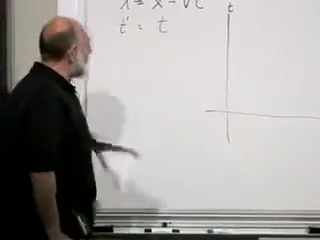
\includegraphics[width=0.72\textwidth]{lecture_04_figure_02.png}\caption{Die galileische Transformation und das anfängliche $t$-$x$-Gitter. Der bewegte Ursprung zeichnet $x=vt$ nach, während die beiden Bezugssysteme gemeinsame Linien konstanter Zeit behalten.}\lectureframe{00:03:06}\end{figure}

Löst man Gl.~\eqref{eq:l4-galilean} nach den ungestrichenen Koordinaten auf, erhält man
\begin{align}
x&=x'+vt'=x'+vt, & t&=t'.
\end{align}
Die inverse Transformation hat dieselbe Form, wenn man $v$ durch $-v$ ersetzt. Bewegt sich der Zug relativ zum Bahnhof vorwärts, so bewegt sich der Bahnhof relativ zum Zug rückwärts. Diese Reziprozität bleibt in der speziellen Relativitätstheorie erhalten, die universelle Zeit jedoch nicht.

\section{Die Lorentz-Korrektur}

Galileische Transformationen können nicht dafür sorgen, dass die Lichtgeschwindigkeit in allen Inertialsystemen gleich ist. Die korrigierten Beziehungen lauten, zunächst in Einheiten mit $c=1$,
\begin{align}
x'&=\frac{x-vt}{\sqrt{1-v^2}}, &
t'&=\frac{t-vx}{\sqrt{1-v^2}}.
\label{eq:l4-lorentz-natural}
\end{align}
Mit den üblichen Einheiten ergibt sich
\begin{align}
x'&=\frac{x-vt}{\sqrt{1-v^2/c^2}}, &
t'&=\frac{t-vx/c^2}{\sqrt{1-v^2/c^2}}.
\label{eq:l4-lorentz-c}
\end{align}

\begin{figure}[H]\centering
\includegraphics[width=0.74\textwidth]{lecture_04_figure_05.png}\caption{Die Lorentz-Transformation mit wieder eingesetzten Faktoren von $c$.}\lectureframe{00:09:10}\end{figure}

Für $v\ll c$ sind sowohl $v^2/c^2$ als auch $vx/c^2$ unter den Bedingungen, unter denen die Newtonsche Mechanik verwendet wird, sehr klein. Gleichung~\eqref{eq:l4-lorentz-c} geht dann in das galileische Ergebnis über. Die Relativitätstheorie verwirft die Newtonsche Kinematik nicht, sondern bestimmt ihren Gültigkeitsbereich.

Bei $v=c$ verschwindet der Nenner. Ein Inertialsystem kann sich relativ zu einem anderen Inertialsystem nicht mit Lichtgeschwindigkeit bewegen. Weit unterhalb dieser Grenze sind die Korrekturen klein; in ihrer Nähe wird die Vermischung von $x$ und $t$ jedoch unvermeidlich.

Die Bewegung wurde entlang $x$ gewählt, daher ändern sich die transversalen Koordinaten nicht:
\begin{equation}
y'=y,\qquad z'=z.
\end{equation}
Warum das so ist, lässt sich folgendermaßen erkennen: Man bringe identische transversale Meterstäbe im Zug und auf dem Bahnsteig an. Ein Beobachter, der sich genau halbwegs zwischen den beiden Bezugssystemen bewegt, sieht die Stäbe mit gleich großen, entgegengesetzten Geschwindigkeiten auf sich zukommen. Nichts an der Anordnung könnte dazu führen, dass einer der beiden transversalen Stäbe kürzer erscheint als der andere.

\section{Lorentz-Transformationen entlang des Lichtkegels}

Gl.~\eqref{eq:l4-lorentz-natural} lässt sich geometrisch deuten. Addiert man die beiden Gleichungen, erhält man
\begin{align}
t'+x'
&=\frac{(t-vx)+(x-vt)}{\sqrt{1-v^2}}\\
&=(t+x)\frac{1-v}{\sqrt{1-v^2}}\\
&=(t+x)\sqrt{\frac{1-v}{1+v}}.
\label{eq:l4-null-plus}
\end{align}
Subtrahiert man sie in der umgekehrten Reihenfolge, ergibt sich
\begin{align}
t'-x'
&=\frac{(t-vx)-(x-vt)}{\sqrt{1-v^2}}\\
&=(t-x)\frac{1+v}{\sqrt{1-v^2}}\\
&=(t-x)\sqrt{\frac{1+v}{1-v}}.
\label{eq:l4-null-minus}
\end{align}

\begin{figure}[H]\centering
\includegraphics[width=0.75\textwidth]{lecture_04_figure_06.png}\caption{Die Lorentz-Transformation, umgeschrieben mit den Nullkombinationen $t+x$ und $t-x$. Ihre Skalierungsfaktoren sind reziprok.}\lectureframe{00:18:45}\end{figure}

Die Kombinationen $t+x$ und $t-x$ sind Koordinaten entlang der beiden lichtartigen Richtungen bei $45^\circ$. Ein Boost staucht eine dieser Richtungen und streckt die andere um den reziproken Faktor. Er dreht keine der beiden aus ihrer Richtung bei $45^\circ$ heraus. Lichtstrahlen bleiben daher Lichtstrahlen – so zeigt sich die Invarianz der Lichtgeschwindigkeit im Raumzeitbild.

\begin{classroomqa}\audiencequestion{Der halbwegs zwischen den Bezugssystemen bewegte Beobachter sieht ein symmetrisches Experiment. Wie lässt sich daraus aber das Ergebnis für die Beobachter im Zug und auf dem Bahnsteig ableiten?\lecturetimestamp{00:20:48}}\lecturerresponse{Dabei wird eine weitere Tatsache vorausgesetzt: Das Zusammenfallen von Ereignissen ist invariant. Treffen die Enden der Stäbe aufeinander, ist dieses Treffen ein einzelnes Raumzeitereignis. Jeder Inertialbeobachter kann ihm andere Koordinaten zuweisen, doch keiner kann ein einziges Zusammentreffen in zwei verschiedene Orte aufspalten. Lichtblitze, die dort ausgesandt werden, wo die entsprechenden Enden zusammentreffen, machen diese Ereignisse beobachtbar. Die Symmetrie im halbwegs bewegten Bezugssystem und die Invarianz der beiden Zusammentreffen an den Enden zeigen, dass die transversalen Längen gleich sind.}\end{classroomqa}

\begin{classroomqa}\audiencequestion{Muss sich der Radfahrer, der das halbwegs bewegte Bezugssystem repräsentiert, tatsächlich in der Mitte zwischen den Stabenden befinden?\lecturetimestamp{00:22:25}}\lecturerresponse{Nein. Ein Bezugssystem ist ein ganzes Netz von Beobachtern und Uhren, nicht ein einzelnes Auge an einem bestimmten Ort. Der Radfahrer kann die Lichtblitze von den Stabenden später empfangen und erschließen, wo sie ausgesandt wurden. Entscheidend ist der Ort jedes Aussendeereignisses in der Raumzeit, nicht der Ort, an dem das Licht schließlich empfangen wird.}\end{classroomqa}

Die Zusammensetzung aufeinanderfolgender Geschwindigkeiten ist eine weitere Folge derselben Transformation, wird aber bewusst der nächsten Vorlesung überlassen. Hier geht es zunächst darum, die invariante Größe zu bestimmen, die eine bewegte Uhr misst.

\section{Das invariante Intervall}

Bei einer Drehung gewöhnlicher kartesischer Achsen bleibt die Größe $x^2+y^2$ unverändert. Lorentz-Transformationen erhalten eine andere quadratische Form. Aus Gl.~\eqref{eq:l4-lorentz-natural} folgt
\begin{align}
t'^2-x'^2
&=\frac{(t-vx)^2-(x-vt)^2}{1-v^2}\\
&=\frac{t^2-2vtx+v^2x^2-x^2+2vtx-v^2t^2}{1-v^2}\\
&=t^2-x^2.
\label{eq:l4-interval}
\end{align}
Die gemischten Terme heben sich auf, und im verbleibenden Zähler lässt sich der gemeinsame Faktor $1-v^2$ ausklammern.

\begin{figure}[H]\centering
\includegraphics[width=0.76\textwidth]{lecture_04_figure_07.png}\caption{Die Herleitung von $t'^2-x'^2=t^2-x^2$ an der Tafel.}\lectureframe{00:33:15}\end{figure}

Mit drei räumlichen Dimensionen lautet die Invariante in Einheiten mit $c=1$
\begin{equation}
t'^2-x'^2-y'^2-z'^2=t^2-x^2-y^2-z^2
\end{equation}
Allgemeiner verwenden wir für zwei Ereignisse Koordinatendifferenzen:
\begin{equation}
\Delta s^2
=c^2\Delta t^2-\Delta x^2-\Delta y^2-\Delta z^2.
\label{eq:l4-spacetime-interval}
\end{equation}
Alle Inertialbeobachter stimmen in diesem Wert überein, auch wenn sie sich über seine getrennten Zeit- und Raumanteile nicht einig sind.

\section{Eigenzeit und bewegte Uhren}

Man stelle sich ein Gitter ruhender Beobachter vor, deren Uhren durch den Austausch von Lichtsignalen synchronisiert wurden. Ihre Anzeigen definieren die Koordinatenzeit $t$. Nun trage man eine Armbanduhr durch dieses Gitter. Ihre eigene Anzeige folgt der Uhr entlang ihrer Weltlinie; diese Anzeige ist die Eigenzeit.

Für zwei zeitartig getrennte Ereignisse definieren wir
\begin{equation}
c^2\Delta\tau^2
=c^2\Delta t^2-\Delta x^2-\Delta y^2-\Delta z^2.
\label{eq:l4-proper-time}
\end{equation}
In einer räumlichen Dimension und mit $c=1$ vereinfacht sich das zu
\begin{equation}
\Delta\tau=\sqrt{\Delta t^2-\Delta x^2}.
\end{equation}
Die Quadratwurzel erinnert an die Formel für einen gewöhnlichen Abstand, doch das Minuszeichen verändert die Geometrie.

Es gibt drei Fälle:
\begin{align}
\Delta t^2-\Delta x^2 &>0 &&\text{timelike},\\
\Delta t^2-\Delta x^2 &=0 &&\text{lightlike},\\
\Delta t^2-\Delta x^2 &<0 &&\text{spacelike}.
\end{align}
Innerhalb des Lichtkegels ist die Eigenzeit reell. Auf dem Lichtkegel, wo $x=\pm t$ gilt, ist sie null, obwohl die Ereignisse nicht zusammenfallen müssen. Ein Lichtstrahl kann genau solche Ereignisse verbinden. Außerhalb des Lichtkegels ist die Trennung raumartig; sie beschreibt man besser durch die reelle Eigenentfernung $\sqrt{\Delta x^2-\Delta t^2}$ als durch eine imaginäre Uhrzeit.

\begin{figure}[H]
\centering
\includegraphics[width=0.73\textwidth]{lecture_04_figure_08.png}

\vspace{0.8em}

\begin{tikzpicture}[x=1.0cm,y=1.0cm]
\draw[->] (-3.3,0) -- (3.3,0) node[right] {$x$};
\draw[->] (0,-0.4) -- (0,4.0) node[above] {$t$};
\draw[thick] (0,0) -- (3.0,3.0) node[above right] {$x=t$};
\draw[thick] (0,0) -- (-3.0,3.0) node[above left] {$x=-t$};
\node at (0,2.0) {timelike};
\node at (2.25,1.05) {spacelike};
\node at (-2.25,1.05) {spacelike};
\end{tikzpicture}\caption{Der Lichtkegel an der Tafel mit einer klaren Einteilung in zeitartige, lichtartige und raumartige Trennungen.}\lectureframe{00:38:40}\end{figure}

Warum entspricht Gl.~\eqref{eq:l4-proper-time} einer Uhrenanzeige? Für eine ruhende Uhr gilt $\Delta x=0$, also $\Delta\tau=\Delta t$. Bei einer gleichförmig bewegten Uhr wählen wir das gestrichene Bezugssystem, in dem diese Uhr ruht. Dort gilt $\Delta x'=0$, und aus der Invarianz folgt
\begin{equation}
\Delta\tau
=\sqrt{\Delta t'^2-\Delta x'^2}
=\Delta t'.
\end{equation}
Bewegte Uhren messen somit die Eigenzeit.

\begin{classroomqa}\audiencequestion{Sind ``das Intervall zwischen den Ereignissen'' und ``die Anzeige der verwendeten Uhr'' zwei Bezeichnungen für dasselbe?\lecturetimestamp{00:44:49}}\lecturerresponse{Sie stimmen überein, wenn eine ideale Uhr sich inertial von einem Ereignis zum anderen bewegt. Das invariante Intervall ist eine geometrische Größe; die Differenz zwischen den Anzeigen der mitbewegten Uhr an den Endpunkten ist ihre physikalische Messung. Eine ruhende Koordinatenuhr zeigt im Allgemeinen ein anderes Koordinatenzeitintervall an.}\end{classroomqa}

\section{Zeitdilatation und Gleichzeitigkeit}

Betrachten wir den Ursprung des bewegten Bezugssystems. Seine Weltlinie erfüllt
\begin{equation}
x'=0,\qquad x=vt.
\end{equation}
Dieselbe schräge Gerade ist sowohl die Bahn der bewegten Uhr als auch die $t'$-Achse.

\begin{figure}[H]\centering
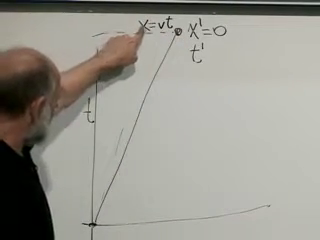
\includegraphics[width=0.72\textwidth]{lecture_04_figure_03.png}\caption{Der bewegte Ursprung: $x=vt$, $x'=0$ und die $t'$-Achse sind drei Beschreibungen derselben Weltlinie.}\lectureframe{00:48:18}\end{figure}

Wenden wir das invariante Intervall auf den gemeinsamen Ursprung und einen späteren Punkt auf dieser Weltlinie an:
\begin{align}
t'^2-x'^2&=t^2-x^2,\\
t'^2&=t^2-v^2t^2,\\
t'&=t\sqrt{1-v^2}.
\label{eq:l4-time-dilation-natural}
\end{align}
Mit wieder eingesetztem $c$ ergibt sich
\begin{equation}
\Delta\tau=\Delta t\sqrt{1-\frac{v^2}{c^2}}
=\frac{\Delta t}{\gamma},
\qquad
\gamma=\frac{1}{\sqrt{1-v^2/c^2}}.
\label{eq:l4-time-dilation}
\end{equation}

\begin{figure}[H]\centering
\includegraphics[width=0.73\textwidth]{lecture_04_figure_09.png}\caption{Das Ergebnis zur Zeitdilatation an der Tafel: Die bewegte Uhr misst in Einheiten mit $c=1$ die Eigenzeit $t'=t\sqrt{1-v^2}$.}\lectureframe{00:50:45}\end{figure}

Der ruhende Beobachter sagt, dass die bewegte Uhr langsamer geht. Aufgrund der Reziprozität muss der bewegte Beobachter dasselbe über ruhende Uhren sagen. Das ist kein Widerspruch, denn die beiden Beschreibungen vergleichen unterschiedliche Paare weit voneinander entfernter Ereignisse.

Tatsächlich erfüllt ein konstanter Wert von $t'$ in Gl.~\eqref{eq:l4-lorentz-natural} die Bedingung
\begin{equation}
t-vx=\text{constant}.
\label{eq:l4-simultaneity}
\end{equation}
Die Gleichzeitigkeitslinien des bewegten Beobachters sind gegenüber den horizontalen Linien $t=\text{constant}$ geneigt. Jeder Beobachter nennt eine andere Auswahl weit voneinander entfernter Uhrenanzeigen gleichzeitig. Berücksichtigt man diesen Unterschied, ist die reziproke Verlangsamung der Uhren widerspruchsfrei.

\begin{figure}[H]\centering
\begin{tikzpicture}[x=1cm,y=1cm]
\draw[->] (0,0) -- (0,4.2) node[above] {$t$};
\draw[->] (0,0) -- (5.2,0) node[right] {$x$};
\draw[thick,->] (0,0) -- (2.4,3.8) node[above] {$x'=0$};
\draw[dashed] (0,2.8) -- (4.8,2.8)
  node[right] {$t=\mathrm{const}$};
\draw[thick] (0.15,1.05) -- (4.7,2.35)
  node[right] {$t'=\mathrm{const}$};
\draw[thick] (3.4,0) -- (3.4,3.8);
\fill (3.4,2.8) circle (0.045);
\fill (3.4,1.98) circle (0.045);
\end{tikzpicture}\caption{Bei der reziproken Zeitdilatation werden Uhrenanzeigen auf unterschiedlichen Gleichzeitigkeitsflächen verglichen.}\end{figure}

\section{Die Wege der Zwillinge}

Zwei Zwillinge beginnen am selben Ereignis. Einer bleibt bei $x=0$. Der andere bewegt sich mit der Geschwindigkeit $v$ nach außen, kehrt um und kommt mit derselben Geschwindigkeit zurück. Bei ihrem Wiedersehen vergleichen sie alle physikalischen Vorgänge, die als Uhr dienen können: Armbanduhren, Herzschlag, Stoffwechsel oder den Alterungsprozess selbst.

Die beiden Reiseabschnitte sollen im Heimatbezugssystem jeweils die Koordinatenzeit $T$ dauern. Die Eigenzeit des zu Hause gebliebenen Zwillings beträgt
\begin{equation}
\tau_{\mathrm{home}}=2T.
\end{equation}
Das Umkehrereignis hat die Koordinaten $(vT,T)$. Der erste Reiseabschnitt trägt daher
\begin{align}
\tau_{\mathrm{leg}}
&=\sqrt{T^2-v^2T^2}
=T\sqrt{1-v^2}.
\end{align}
bei. Der Rückweg trägt denselben Betrag bei, also
\begin{equation}
\tau_{\mathrm{travel}}=2T\sqrt{1-v^2}<2T.
\label{eq:l4-twin}
\end{equation}

\begin{figure}[H]
\centering
\includegraphics[width=0.73\textwidth]{lecture_04_figure_10.png}

\vspace{0.8em}

\begin{tikzpicture}[x=1.1cm,y=1cm]
\draw[->] (-0.2,0) -- (3.4,0) node[right] {$x$};
\draw[->] (0,-0.1) -- (0,4.4) node[above] {$t$};
\draw[very thick] (0,0) -- (0,4);
\draw[very thick] (0,0) -- (2.2,2) -- (0,4);
\draw[dashed] (0,2) -- (2.2,2);
\node[left] at (0,2) {$T$};
\node[left] at (0,4) {$2T$};
\node[below right] at (1.1,1.0) {$v$};
\node[above right] at (1.1,3.0) {$-v$};
\end{tikzpicture}\caption{Die Weltlinie des zu Hause gebliebenen Zwillings und die beiden Reiseabschnitte. Ihre Eigenzeiten unterscheiden sich, weil sie verschiedenen Wegen durch die Raumzeit folgen.}\lectureframe{00:59:35}\end{figure}

Die unterschiedlichen Altersangaben sind kein Widerspruch. Der Reiseweg enthält eine Umkehr und ist nicht durch eine einzige Symmetrie zwischen Inertialsystemen mit der geraden Weltlinie des zu Hause gebliebenen Zwillings verknüpft. Auch in der gewöhnlichen euklidischen Geometrie sind die Längen einer geraden Strecke und eines geknickten Weges zwischen zwei Punkten verschieden. In der Minkowski-Geometrie kehrt sich um, welcher Weg das größere Intervall hat; der Vergleich bleibt jedoch geometrisch.

\section{Beschleunigung und die ideale Uhr}

\begin{classroomqa}\audiencequestion{Bei der Umkehr ist die Physik anders, und der Reisende wird beschleunigt. Macht das die Uhrenberechnung ungültig?\lecturetimestamp{01:02:19}}\lecturerresponse{Die Beschleunigung ist real und hilft, die Asymmetrie zu erkennen; man sollte sie nicht wegargumentieren. Die scharfe Ecke ist nur eine idealisierte Zeichnung und lässt sich durch eine endliche Umkehr mit abgerundetem Verlauf ersetzen. Hinzu kommt die physikalische Annahme, dass eine hinreichend kleine, gut gebaute Uhr gegenüber mäßiger Beschleunigung unempfindlich ist und weiterhin die Eigenzeit anzeigt. Eine große oder empfindliche Uhr kann sich verformen oder kaputtgehen; das wäre jedoch ein Mangel des Mechanismus und nicht des Raumzeitintervalls.}\end{classroomqa}

Diese Annahme über ideale Uhren folgt nicht allein aus der Lorentz-Transformation. Sie wird anhand des Verhaltens tatsächlicher Uhrenmechanismen geprüft. Ein Atom ist eine viel bessere Näherung als eine Uhr, die Hunderte von Meilen groß ist, denn der kompakte Mechanismus lässt sich durch Beschleunigung oder Gravitation schwerer verformen. Die allgemeine Relativitätstheorie beim Namen zu nennen, beseitigt dieses physikalische Problem nicht; man müsste weiterhin wissen, wie der gewählte Mechanismus auf seine Umgebung reagiert.

\begin{classroomqa}\audiencequestion{Lässt sich eine beschleunigte Bahn in kurze Abschnitte zerlegen, für die die Inertialanalyse weiterhin gilt?\lecturetimestamp{01:09:08}}\lecturerresponse{Ja. Man zerlegt die Kurve in kurze, nahezu gerade Abschnitte, berechnet für jeden die Eigenzeit und addiert die Ergebnisse. Das entspricht in der Raumzeit der Bestimmung der Länge einer gewöhnlichen Kurve aus vielen kleinen geraden Strecken. Im Kontinuumslimes gilt für eine Bewegung in der flachen Raumzeit, beschrieben in einem Inertialkoordinatensystem,
\[
\tau=\int \sqrt{1-\frac{v(t)^2}{c^2}}\,dt,
\]}\end{classroomqa}

\section{Was die Zwillinge sehen}

Die endgültigen Uhrenanzeigen lassen sich durch das Aussenden von Lichtblitzen operational zugänglich machen. Auf beiden Weltlinien markiert man Intervalle von einer Sekunde Eigenzeit und lässt jeden Zwilling bei jeder Markierung einen Lichtblitz aussenden. Während des Hinwegs treffen die vom jeweils anderen Zwilling empfangenen Blitze in größeren Abständen ein. Auf dem Rückweg kommen sie gehäuft an. Das ist der relativistische Doppler-Effekt, direkt im Raumzeitdiagramm dargestellt.

\begin{figure}[H]\centering
\includegraphics[width=0.73\textwidth]{lecture_04_figure_11.png}\caption{Zwischen der Weltlinie des zu Hause gebliebenen und der des reisenden Zwillings ausgetauschte Lichtsignale. Die größeren Abstände der empfangenen Blitze auf dem Hinweg und ihre Verdichtung auf dem Rückweg erklären jeden ausgesandten Blitz.}\lectureframe{01:12:55}\end{figure}

Keine Bezugssysteme verschwinden aus der Darstellung. Jeder Beobachter empfängt schließlich alle Blitze, die der andere ausgesandt hat; die Empfangsrate hängt jedoch von der Relativbewegung ab. Für die beiden Wege wirken Rotverschiebung auf dem Hinweg und Blauverschiebung auf dem Rückweg unterschiedlich lange. Daher stimmt die Zählung aller empfangenen Blitze mit dem Vergleich der Eigenzeiten überein.

\begin{classroomqa}\audiencequestion{Wenn der zurückkehrende Reisende blauverschobenes Licht empfängt, könnte er dann mehr Energie erhalten, als die Quelle ausgesandt hat?\lecturetimestamp{01:13:50}}\lecturerresponse{Diese Frage erfordert die relativistische Definition der Energie und die Berücksichtigung ihrer Abhängigkeit vom Bezugssystem; beides wurde noch nicht entwickelt. Die Frage ist berechtigt, doch Koordinaten und die Anzahl der Lichtblitze reichen allein nicht aus, um die Energiebilanz zu klären, insbesondere für einen beschleunigten Beobachter. Die Antwort sollte daher aufgeschoben und nicht erraten werden.}\end{classroomqa}

\section{Eine geschlossene räumliche Richtung}

\begin{classroomqa}\audiencequestion{Angenommen, eine räumliche Richtung sei kompakt. Könnte sich ein Zwilling gleichförmig auf ihr bewegen, zum Ausgangsort zurückkehren und dabei jede Beschleunigung vermeiden? Was würde die Zwillinge dann unterscheiden?\lecturetimestamp{01:15:14}}\lecturerresponse{Der Raum ist intrinsisch als Zylinder vorzustellen, nicht als Fläche, die in einen größeren Raum hineingebogen ist; eine radiale Beschleunigung muss es nicht geben. Der zurückkehrende Beobachter begegnet dennoch der globalen Tatsache, dass dieselben Orte wiederkehren. Das deutet auf eine Asymmetrie hin, doch eine vollständige Antwort erfordert eine sorgfältige Behandlung der speziellen Relativitätstheorie mit dieser räumlichen Identifikation. Die Frage bleibt hier offen, statt spontan beantwortet zu werden.}\end{classroomqa}

\begin{figure}[H]
\centering
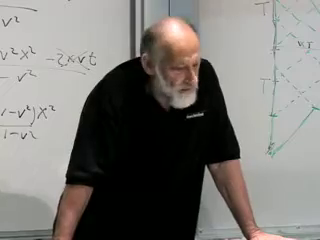
\includegraphics[width=0.72\textwidth]{lecture_04_figure_04.png}

\vspace{0.8em}

\begin{tikzpicture}[x=1cm,y=1cm]
\draw[thick] (0,0) ellipse (1.3 and 0.35);
\draw[thick] (-1.3,0) -- (-1.3,-3.1);
\draw[thick] (1.3,0) -- (1.3,-3.1);
\draw[thick] (0,-3.1) ellipse (1.3 and 0.35);
\draw[->,very thick] (0.0,0.38) arc (90:-210:1.38 and 0.42);
\node[right] at (1.65,-1.5) {compact spatial direction};
\end{tikzpicture}\caption{Die Frage zum kompakten Raum, wie an der Tafel gezeichnet, mit einem sauberen intrinsischen Zylinder. Es geht um eine globale Identifikation, nicht um Bewegung auf einem Zylinder, der in eine zusätzliche radiale Dimension eingebettet ist.}\lectureframe{01:17:56}\end{figure}

\section{Längen werden auf einer Gleichzeitigkeitsfläche gemessen}

Bei einem Problem der speziellen Relativitätstheorie zeichnet man zuerst das Raumzeitbild. Betrachten wir einen Meterstab, der im ungestrichenen Bezugssystem ruht und dessen Endpunkte bei $x=0$ und $x=1$ liegen. Mit der Zeit zeichnen seine beiden Endpunkte vertikale Weltlinien. Der Stab überstreicht ein Band in der Raumzeit.

Der bewegte Beobachter muss beide Endpunkte bei demselben Wert der bewegten Zeit $t'$ messen. Aus Gl.~\eqref{eq:l4-simultaneity} folgt, dass die Fläche durch den Ursprung mit $t'=0$ die Bedingung
\begin{equation}
t=vx
\end{equation}
erfüllt, in Einheiten mit $c=1$. Sie schneidet die Weltlinie des rechten Endpunkts $x=1$ bei $t=v$.

\begin{figure}[H]
\centering
\includegraphics[width=0.73\textwidth]{lecture_04_figure_12.png}

\vspace{0.8em}

\begin{tikzpicture}[x=1.55cm,y=1.15cm]
\draw[->] (-0.5,0) -- (3.1,0) node[right] {$x$};
\draw[->] (0,0) -- (0,3.8) node[above] {$t$};
\draw[very thick,red] (0,0) -- (0,3.3);
\draw[very thick,red] (2.15,0) -- (2.15,3.3);
\fill[red!12] (0,0) rectangle (2.15,3.3);
\draw[very thick,green!50!black] (0,0) -- (1.2,3.1)
  node[above] {$x=vt$};
\draw[very thick,blue] (0,0) -- (2.15,1.15)
  node[right] {$t'=0$};
\fill (2.15,1.15) circle (0.045);
\node[right] at (2.22,1.35) {$(x,t)=(1,v)$};
\node[below] at (2.15,0) {$1$};
\end{tikzpicture}\caption{Ein ruhender Stab überstreicht ein Band in der Raumzeit. Die vom bewegten Beobachter gemessene Länge ist der Abstand zwischen seinen Endpunkten auf einer Fläche mit konstantem $t'=\mathrm{const}$.}\lectureframe{01:24:20}\end{figure}

Der gewählte Abstand zwischen den Endpunkten ist raumartig; daher verwendet man die positive räumliche Form der Invariante:
\begin{equation}
x'^2-t'^2=x^2-t^2.
\end{equation}
Am gewählten Endpunkt gilt $t'=0$, $x=1$ und $t=v$. Somit
\begin{align}
x'^2&=1-v^2,\\
x'&=\sqrt{1-v^2}.
\end{align}
Eine Ruhelänge $L$ wird im bewegten Bezugssystem also als
\begin{equation}
L'=L\sqrt{1-v^2/c^2}=\frac{L}{\gamma}.
\label{eq:l4-length-contraction}
\end{equation}
gemessen.

\begin{figure}[H]\centering
\includegraphics[width=0.76\textwidth]{lecture_04_figure_13.png}\caption{Die vollständige Herleitung der Längenkontraktion und das Ergebnis an der Tafel $x'=\sqrt{1-v^2}$ für eine Ruhelänge von einer Einheit.}\lectureframe{01:28:10}\end{figure}

Auch die reziproke Aussage gilt: Der Beobachter auf dem Bahnsteig schreibt dem längs ausgerichteten Meterstab im Zug eine kürzere Länge zu. Wieder wählen die beiden Beobachter unterschiedliche gleichzeitige Ereignisse an den Endpunkten; daher ist die Reziprozität kein Widerspruch.

\section{Fragen zum Abschluss}

\begin{classroomqa}\audiencequestion{Breitet sich außer Licht noch etwas mit Lichtgeschwindigkeit aus? Was ist insbesondere mit der Gravitation?\lecturetimestamp{01:29:29}}\lecturerresponse{Die allgemeine Relativitätstheorie sagt Gravitationswellen voraus, die sich mit $c$ ausbreiten. Zum Zeitpunkt dieser Vorlesung stammten die Belege indirekt aus Systemen wie Doppelsternpulsaren; Gravitationswellen waren noch nicht direkt nachgewiesen worden.\editorialnote{Die experimentelle Lage änderte sich nach dieser Vorlesung von 2006. LIGO wies GW150914 im Jahr 2015 direkt nach, und die gemeinsame Beobachtung von GW170817 und seinem elektromagnetischen Gegenstück im Jahr 2017 zeigte, dass die Ausbreitungsgeschwindigkeiten von Gravitation und Licht bis auf wenige Teile von $10^{15}$ übereinstimmen. Siehe \url{https://ligo.org/detections/gw150914/} und \url{https://doi.org/10.1103/PhysRevLett.119.251302}.}}\end{classroomqa}

\begin{classroomqa}\audiencequestion{Kann ein Astronaut eine Entfernung von vielen Lichtjahren in weniger Eigenzeit durchqueren, als die in Lichtjahren angegebene Entfernung beträgt? Würde das bedeuten, dass er sich schneller als Licht bewegt?\lecturetimestamp{01:30:38}}\lecturerresponse{Die Eigenzeit des Astronauten beträgt $\sqrt{\Delta t^2-\Delta x^2}$; sie ist kleiner als die Koordinatenzeit $\Delta t$. Im Inertialsystem des Astronauten ist der Abstand zwischen den Sternen lorentzkontrahiert. Die Sterne bewegen sich mit der Geschwindigkeit $-v$, nicht schneller als Licht; es ist schlicht eine kürzere, kontrahierte Strecke zu durchqueren.}\end{classroomqa}

Beginnt der Astronaut aus dem Ruhezustand und beschleunigt, ändert sich die Beschreibung von einem momentanen Inertialsystem zum nächsten. Der den Sternen zugewiesene Abstand kann sich während dieses Übergangs ändern. Man kann nicht eine einzige feste Lorentz-Transformation auf die gesamte beschleunigte Geschichte anwenden; die gesamte Eigenzeit ergibt sich dennoch durch Addition der Beiträge entlang der Weltlinie. Dasselbe gilt für einen realistischen Zwilling, der startet, umkehrt und abbremst, statt mit Reisegeschwindigkeit geboren zu werden.

\begin{classroomqa}\audiencequestion{Entstehen diese Rätsel dadurch, dass die Zeit als etwas Besonderes behandelt wird? Müssen wir sie eine vierte Dimension nennen?\lecturetimestamp{01:36:43}}\lecturerresponse{Man muss nicht mit dem Schlagwort beginnen, die Zeit sei eine vierte Dimension. Die Lorentz-Transformation selbst erzwingt eine Vermischung von Raum und Zeit, während das Intervall $t^2-x^2-y^2-z^2$ sie als Bestandteile einer einzigen Geometrie auffasst, wobei für Zeit und Raum unterschiedliche Vorzeichen gelten. Bei niedriger Geschwindigkeit wird die Vermischung vernachlässigbar, und die vertraute Newtonsche Intuition kehrt zurück. Bei relativistischen Geschwindigkeiten lassen sich Raum und Zeit jedoch nicht als grundsätzlich entkoppelt betrachten.}\end{classroomqa}

Zeitdilatation, Längenkontraktion, der Vergleich der Zwillinge und die verkürzte Reisezeit sind also keine voneinander unabhängigen Tricks. Sie folgen alle aus drei Vorgehensweisen: die verglichenen Ereignisse bestimmen, ihre Raumzeitgeometrie zeichnen und das invariante Intervall verwenden.
\chapter{Feuerbälle, Bezugssysteme und Vierervektoren}

Wir beginnen mit einer Frage, die nach der Diskussion hochenergetischer Kollisionen offen geblieben ist. Bei der Kollision zweier schwerer Atomkerne entsteht ein heftig veränderliches Objekt, kein ruhiges astronomisches Schwarzes Loch. Was kann es also bedeuten, die Kollision mithilfe eines Horizonts zu beschreiben? Die Antwort führt über ein fünfdimensionales Bild stark gekoppelter Materie und einige praktische Fragen zu Beschleunigern schließlich zurück zur Geometrie der speziellen Relativitätstheorie. Am Ende sind Geschwindigkeit und Impuls zu Vierervektoren geworden, und die Energie steht neben den drei Impulskomponenten.

\section{Ein Feuerball in einer fünften Dimension}

\begin{classroomqa}
\audiencequestion{Das bei der Kollision entstehende Objekt ist instabil und verändert seine Form. Wie kann man ein so komplexes Objekt als Schwarzes Loch bezeichnen?}
\lecturerresponse{Stellen wir uns eine fünfte räumliche Richtung zwischen einem Boden und einer Decke vor. Die Gravitation in dieser Richtung zieht Anregungen zum Boden hin. Bei der Kollision wird dort ein heißer Energieklumpen abgelagert; er breitet sich aus und verändert seine Form, kann aber dennoch einen Horizont, eine Temperatur und eine Entropie besitzen.}
\end{classroomqa}

Stellen wir uns Teilchen oder, anschaulicher, kleine Strings vor, die sich in dieser fünfdimensionalen Welt bewegen. Anregungen, die zum Boden fallen, erscheinen in vier Dimensionen als Hadronen: Protonen, Neutronen, Mesonen und andere ausgedehnte zusammengesetzte Objekte. Anregungen nahe der Decke erscheinen elementarer. Die vertikale Position kodiert somit die Skala auf geometrische Weise: Der Boden steht für den hadronischen Bereich großer Abstände, die Decke für Freiheitsgrade bei kleinen Abständen.

Wenn zwei Hadronen kollidieren, stoßen zwei Objekte nahe dem Boden zusammen und erzeugen eine große Energiefreisetzung. Das Ergebnis ist kein starrer Körper, sondern ein heißer Klumpen mit Horizont, eine Art Pfütze im fünfdimensionalen Gravitationsfeld. Es ist weder ein astronomisches Schwarzes Loch im gewöhnlichen vierdimensionalen Raum noch ein Schwarzes Loch auf der Planck-Skala, das an der Decke sitzt. Es ist die gravitative Beschreibung des stark wechselwirkenden Feuerballs nahe dem Boden.

Bei hohen Energien werden die einlaufenden Atomkerne lorentzkontrahiert und zu dünnen Pfannkuchen. Sie kollidieren, deponieren ihre Energie in einem kleinen Gebiet und erzeugen ein Fluid, das sich zum Gleichgewicht hin ausbreitet. Seine geringe Viskosität war eine der überraschenden Eigenschaften des Quark--Gluon-Plasmas. In der fünfdimensionalen Beschreibung entspricht dieselbe Entwicklung der Relaxation eines verzerrten Horizonts.

\begin{figure}[H]
\centering
\includegraphics[width=0.82\textwidth]{lecture_05_figure_01.png}
\caption{Das Bild der fünften Dimension mit Boden und Decke. Der zentrale Klumpen mit Horizont breitet sich nach der Kollision entlang des Bodens aus.}
\lectureframe{00:04:22}
\end{figure}

Ein Horizont bleibt nicht ewig bestehen. Hawking-Strahlung trägt Energie davon, und in der vierdimensionalen Beschreibung ist diese Strahlung der Schauer gewöhnlicher Hadronen, die aus der Kollision hervorgehen. Die Tausenden Spuren in einem Detektorereignis sind in dieser Sprache die Teilchen, die aus dem dualen Schwarzen Loch herausgesiedet sind.

\subsection{Ist die zusätzliche Dimension real?}

\begin{classroomqa}
\audiencequestion{Ist die fünfte Dimension eine räumliche Dimension, und erstreckt sich die zwischen Boden und Decke gezeichnete Linie buchstäblich in diese Richtung?}
\lecturerresponse{Ja. Sie ist raumartig, und die in dieser fünfdimensionalen Geometrie gezeichnete Fläche ist ein Horizont. Ob man die zusätzliche Richtung als ``real'' bezeichnet oder sie als gleichwertige mathematische Beschreibung auffasst, ist eine tiefer gehende Frage.}
\end{classroomqa}

Die nützliche Aussage lautet nicht, dass die Gravitation die Quantenchromodynamik ersetzt. Vielmehr können zwei Sprachen dieselbe Physik beschreiben. In der vierdimensionalen Sprache gibt es einen heißen Feuerball aus Quarks und Gluonen, aber kein gewöhnliches Gravitationsfeld. In der fünfdimensionalen Sprache gibt es Gravitation und einen Horizont. Wenn die Korrespondenz stimmt, müssen eine korrekte QCD-Rechnung und die duale Gravitationsrechnung überall dort übereinstimmen, wo sich beide durchführen lassen.

\begin{classroomqa}
\audiencequestion{QCD kennt weder Gravitation noch Horizonte. Fügt das Bild des Schwarzen Lochs neue Physik hinzu, oder beschreibt es den Feuerball lediglich anders?}
\lecturerresponse{In vier Dimensionen ist es ein Plasma aus Quarks und Gluonen; in seiner fünfdimensionalen Ausprägung besitzt es eine gravitative Beschreibung mit einem Horizont. Der Vorteil liegt in der Berechnung. Stark gekoppelte QCD ist äußerst schwierig, während sich manche Eigenschaften des Horizonts---insbesondere die Viskosität---vergleichsweise leicht berechnen lassen.}
\end{classroomqa}

Die Frage, ob es sich um eine ``reale Dimension'' oder eine ``mathematische Analogie'' handelt, muss nicht geklärt werden, bevor die Beschreibung nützlich sein kann. Eine Struktur erhält eine physikalische Deutung, wenn sie die übrigen Variablen zu einem einfacheren und kohärenteren Satz von Gesetzen zusammenführt. Dennoch sollte man die Aussage nicht übertreiben: Anwendungen der Eich-Gravitation-Dualität auf das beobachtete Quark--Gluon-Plasma sind Modelle stark gekoppelter Dynamik und kein Beweis dafür, dass es für die QCD der realen Welt ein bekanntes exaktes gravitationelles Dual gibt.\editorialnote{Diese Einschränkung macht den heutigen Stand der QCD-Anwendung ausdrücklich deutlich; sie ändert nichts am hier entwickelten fünfdimensionalen Mechanismus.}

\section{Warum Beschleuniger kollidierende Strahlen verwenden}

Nun werden die Fragen praktisch. Warum verwendet man zwei bewegte Strahlen statt eines einzelnen Strahls und eines ruhenden Ziels? Warum sind kreisförmige Beschleuniger so groß? Warum geht man mit Elektronen und Protonen unterschiedlich um? All diese Fragen betreffen relativistische Energie.

\begin{classroomqa}
\audiencequestion{Warum lässt man zwei Strahlen miteinander kollidieren, statt einen energiereichen Strahl auf ein ruhendes Ziel zu richten?}
\lecturerresponse{Für die Erzeugung neuer Teilchen ist die im Schwerpunktsystem verfügbare Energie maßgeblich. Zwei gleich starke, entgegengesetzt gerichtete relativistische Strahlen haben keinen Gesamtimpuls, sodass im Wesentlichen ihre gesamte Energie für die Kollision zur Verfügung steht. Bei einem ruhenden Ziel bleibt ein großer Teil der einfallenden Energie als Bewegung des Schwerpunkts gebunden.}
\end{classroomqa}

Für zwei ultrarelativistische Teilchen mit entgegengesetzten Impulsen vom Betrag \(p\) lautet die Abschätzung auf Vorlesungsniveau in Einheiten mit \(c=1\)
\begin{equation}
E_{\mathrm{cm}}^{\mathrm{collider}}\simeq 2p.
\end{equation}
Die entsprechende Abschätzung für ein ruhendes Ziel wächst nur mit der Quadratwurzel des Strahlimpulses:
\begin{equation}
E_{\mathrm{cm}}^{\mathrm{fixed}}\sim \sqrt{mp}.
\end{equation}
Entscheidend ist die Skalierung, nicht der weggelassene Zahlenfaktor: Eine Verdopplung der Strahlenergie verdoppelt die Kollisionsenergie des Beschleunigers, erhöht die Schwerpunktsenergie beim ruhenden Ziel aber nur um einen Faktor gleich der Quadratwurzel.

Die invariante Rechnung macht den Vergleich präzise. Sind \(P_1\) und \(P_2\) die einlaufenden Viererimpulse, gilt
\begin{equation}
s=(P_1+P_2)^2,
\qquad E_{\mathrm{cm}}=\sqrt{s}.
\end{equation}
Für zwei gleichenergetische, entgegengesetzt laufende Strahlen mit Energie \(E\) heben sich die räumlichen Impulse auf, sodass \(\sqrt{s}=2E\) gilt. Für ein Projektil der Energie \(E\gg m\), das auf ein ruhendes Ziel gleicher Masse trifft, gilt
\begin{equation}
s=2m^2+2mE,
\qquad
\sqrt{s}\simeq \sqrt{2mE}
\qquad (c=1).
\end{equation}
Diese kurze Herleitung mit Invarianten liefert den Faktor, der in der mündlichen Abschätzung unterdrückt wurde.\editorialnote{Die Herleitung ist hier aufgenommen, damit sich das Skalierungsargument der Vorlesung nachvollziehen lässt.}

\begin{classroomqa}
\audiencequestion{Gibt es einen grundlegenden Grund dafür, dass ein kreisförmiger Beschleuniger so groß sein muss? Könnte derselbe Strahl nicht einfach öfter durch eine kleinere Maschine kreisen?}
\lecturerresponse{Felder und Materialien setzen Grenzen. Ein Teilchen gewinnt pro Meter nur eine begrenzte Energie, daher braucht eine Maschine für höhere Energien eine größere wirksame Beschleunigungsstrecke. Ein enger Kreis erfordert zudem eine größere Querbeschleunigung, und eine beschleunigte Ladung strahlt. Ist der Ring zu klein, strahlt der Strahl Energie genauso schnell ab, wie die Maschine sie zuführt.}
\end{classroomqa}

Die Beziehung für die Ablenkung lautet näherungsweise
\begin{equation}
p=qBR,
\end{equation}
Bei festem Magnetfeld \(B\) erfordert ein größerer Impuls \(p\) also einen größeren Radius \(R\). Die Hochfrequenzkavitäten verrichten die Arbeit, die die Strahlenergie erhöht; die Magnete lenken den Strahl ab und fokussieren ihn. Die grundsätzliche Aussage bleibt die an der Tafel erläuterte: Die Feldstärke und die Strahlungsverluste hindern uns daran, einen beliebig energiereichen Beschleuniger in einen kleinen Ring zu packen.

Bei einer Kreisbewegung tritt auch bei konstanter Geschwindigkeit eine Beschleunigung auf, denn die Geschwindigkeit ändert ihre Richtung. Eine beschleunigte Ladung sendet Synchrotronstrahlung aus. Ein Linearbeschleuniger vermeidet den kontinuierlichen Ablenkungsverlust, auch wenn die kurzen Beschleunigungsstöße selbst nicht buchstäblich strahlungsfrei sind. Kreisförmige Maschinen nehmen die Kosten der Ablenkung in Kauf und verwenden dafür bei jedem Umlauf dieselbe Anlage erneut.

\begin{classroomqa}
\audiencequestion{Warum wurden Elektronen mit dem Linearbeschleuniger am SLAC in Verbindung gebracht, während kreisförmige Hochenergie-Collider Protonen oder andere Hadronen verwenden?}
\lecturerresponse{Elektronen sind viel leichter. Bei gleicher hoher Energie ist ihr Lorentzfaktor deutlich größer, und bei kreisförmiger Beschleunigung strahlen sie viel stärker. Schwerere Protonen können wiederholt im Kreis laufen und bei jedem Umlauf Energie gewinnen, bevor Synchrotronverluste untragbar werden.}
\end{classroomqa}

Bei gleicher Energie und gleichem Ringradius hängt die Strahlungsleistung sehr stark von der Teilchenmasse ab:
\begin{equation}
P_{\mathrm{sync}}\propto \frac{E^4}{m^4R^2}.
\end{equation}
Darum ist der Unterschied zwischen Elektronen und Protonen--deutlich ausgeprägter, als die Formulierung ``das leichtere Teilchen bewegt sich schneller'' vermuten lässt: Beide Strahlen können bereits sehr nahe an \(c\) liegen, aber ihre Lorentzfaktoren und Strahlungsverluste unterscheiden sich stark.\editorialnote{Die Ablenkungsbeziehung und die Skalierung der Synchrotronstrahlung präzisieren das qualitative Argument der Vorlesung zu Beschleunigern; an der Tafel wurden sie nicht hergeleitet.}

\begin{classroomqa}
\audiencequestion{Warum beschleunigt man Hadronen nicht ebenfalls geradlinig?}
\lecturerresponse{Das ist möglich. Die Schwierigkeit liegt in der Länge. In einem Ring durchläuft dasselbe Teilchen die Beschleunigungsstrukturen viele Male; eine gleichwertige lineare Hadronenmaschine müsste enorm lang sein. Ein sinnvoller Kompromiss ist ein großer Ring, groß genug, damit die Protonenstrahlung erträglich bleibt.}
\end{classroomqa}

Diese Fragen zu Beschleunigern machen genau deutlich, weshalb die Newtonsche Mechanik nicht ausreicht. Wir wenden uns nun wieder der speziellen Relativitätstheorie zu und entwickeln die Sprache, mit der sich solche Vergleiche systematisch führen lassen.

\section{Die Garage und die Limousine}

Betrachten wir eine etwa zwölf Fuß lange Garage und eine etwa zwanzig Fuß lange Stretchlimousine. Der Fahrer beschleunigt, bis die Limousine lorentzkontrahiert ist, und hofft, dass sie hineinpasst. Im Bezugssystem der Garage ist die bewegte Limousine kürzer, sodass es möglich erscheint. Im Bezugssystem der Limousine dagegen ist die bewegte Garage kürzer, sodass es unmöglich erscheint. Kann sich die gesamte Limousine in der Garage befinden?

Öffnen wir beide Tore, damit uns eine mögliche Kollision mit einer Wand nicht ablenkt. Die Aussage, dass sich die Limousine in der Garage befindet, bedeutet, dass sich ihr Vorder- und Hinterende \emph{gleichzeitig} in der Garage befinden. Dieses letzte Wort enthält das ganze Rätsel.

Zeichnen wir ein Raum-Zeit-Diagramm mit \(t\) als vertikaler und \(x\) als horizontaler Achse. Lichtstrahlen bilden in Einheiten mit \(c=1\) einen Lichtkegel mit Öffnungswinkel \(45^\circ\). Die Garage ruht, daher sind die Weltlinien ihrer beiden Tore vertikal. Vorder- und Hinterende der Limousine beschreiben zwei parallele, schräge Weltlinien. Die \(t'\)-Achse des bewegten Bezugssystems ist zum Lichtkegel hin geneigt, und seine Simultanitätslinien verlaufen parallel zur geneigten \(x'\)-Achse.

\begin{figure}[H]
\centering
\includegraphics[width=0.82\textwidth]{lecture_05_figure_02.png}
\caption{Das vollständige Raum-Zeit-Diagramm für Garage und Limousine. Vertikale Linien begrenzen die Garage; schräge Linien zeichnen die beiden Enden der Limousine nach. Horizontale und geneigte Schnitte stellen die unterschiedlichen Simultanitätsebenen der beiden Bezugssysteme dar.--}
\lectureframe{00:31:05}
\end{figure}

Im Bezugssystem der Garage kann eine horizontale Linie beide Weltlinien der Limousine zwischen den beiden Weltlinien der Garagentore schneiden. Zu diesem Zeitpunkt im Garagenbezugssystem ist das Heck bereits eingefahren, während die Front noch nicht wieder hinausgefahren ist. Die kontrahierte Limousine befindet sich vollständig in der Garage.

Im Bezugssystem der Limousine liegen die relevanten gleichzeitigen Ereignisse auf einer geneigten Linie. Zeichnen wir eine solche Linie durch das Ereignis, bei dem das Heck einfährt. Sie trifft die Weltlinie der Front, nachdem diese bereits am weiter entfernten Tor vorbeigefahren ist. Nach der für sie maßgeblichen Gleichzeitigkeit befindet sich die Limousine also niemals vollständig in der Garage. Beide Aussagen sind wahr, weil sie jeweils unterschiedliche Ereignispaare vergleichen.

\begin{classroomqa}
\audiencequestion{Bilden die beiden grünen Weltlinien und das horizontale Segment zwischen ihnen ein Parallelogramm? Ist dieses schwarze Segment die Länge des Fahrzeugs?}
\lecturerresponse{Das horizontale Segment ist die lorentzkontrahierte Länge, denn seine Endpunkte sind im Bezugssystem der Garage gleichzeitig. Die Ruhelänge erhält man mit Endpunkten, die im Bezugssystem der Limousine gleichzeitig sind, auf einer Linie parallel zu \(x'\). Die beiden Messungen verwenden unterschiedliche Schnitte durch dasselbe Weltlinienpaar.}
\end{classroomqa}

Ist \(L_0\) die Ruhelänge, dann hat der horizontale Schnitt im Bezugssystem der Garage die Länge
\begin{equation}
L=\frac{L_0}{\gamma},
\qquad
\gamma=\frac{1}{\sqrt{1-v^2/c^2}}.
\end{equation}
Die Formel allein löst das Paradoxon nicht. Das leistet das Diagramm, weil es zeigt, welche Ereignisse miteinander verglichen wurden. Scheint ein Relativitätsrätsel zwei unvereinbare Antworten zu liefern, sollte man nach einer unausgesprochenen Verwendung des Wortes ``gleichzeitig'' suchen.

\section{Vier Koordinaten und zwei Indexstellungen}

Um von Rätseln zu Bewegungsgesetzen überzugehen, brauchen wir eine Notation, die die Geometrie berücksichtigt. Wir fassen die Koordinaten wie folgt zusammen:
\begin{equation}
(X^1,X^2,X^3,X^0)=(x,y,z,t),
\qquad X^\mu=(x,y,z,t),
\end{equation}
Dabei durchläuft \(\mu\) die Werte \(1,2,3,0\). Auf der Seite steht die Zeit an letzter Stelle, obwohl ihr Index \(0\) ist; damit folgen wir der Konvention an der Tafel.

\begin{classroomqa}
\audiencequestion{Setzen wir \(c=1\)? Sollte bei Rückkehr zu den üblichen Einheiten die Zeitkoordinate \(ct\) lauten?}
\lecturerresponse{Ja. Bei der Entwicklung der Geometrie setzen wir \(c=1\) und fügen die Faktoren \(c\) wieder ein, wenn Dimensionen oder der nichtrelativistische Grenzfall eine Rolle spielen. In den üblichen Längeneinheiten lautet die Zeitkoordinate \(ct\).}
\end{classroomqa}

Derselbe Vektor lässt sich auch mit einem unteren Index schreiben. Bei der hier verwendeten Vorzeichenkonvention gilt
\begin{equation}
X_\mu=(-x,-y,-z,t).
\end{equation}
Beim Senken eines Index wechseln also die Vorzeichen der drei räumlichen Komponenten, während die Zeitkomponente unverändert bleibt. Zum Beispiel:
\begin{equation}
X^\mu=(3,2,4,10)
\quad\Longrightarrow\quad
X_\mu=(-3,-2,-4,10).
\end{equation}
Das sind keine zwei Raum-Zeit-Punkte, sondern zwei Komponentendarstellungen desselben geometrischen Objekts.

\begin{classroomqa}
\audiencequestion{Welche Komponenten sind kovariant und welche kontravariant, und sind die Bezeichnungen als Hoch- oder Tiefstellungen gemeint?}
\lecturerresponse{Komponenten mit oberen Indizes sind kontravariant, solche mit unteren Indizes kovariant. Als Eselsbrücke aus dem Hörsaal gilt: ``co steht unten, kontra steht oben.'' Physiker sagen oft einfach „oben“ und „unten“.}
\end{classroomqa}

Die Notation bewährt sich bei der invarianten Kontraktion
\begin{equation}
X_\mu X^\mu=t^2-x^2-y^2-z^2.
\label{eq:l5-interval}
\end{equation}
In Differentialform lautet sie
\begin{equation}
d\tau^2=dt^2-dx^2-dy^2-dz^2
\qquad (c=1).
\label{eq:l5-proper-time}
\end{equation}
Bei zeitartiger Bewegung ist \(d\tau\) die Zeit, die eine Uhr entlang der Weltlinie misst.

Tritt derselbe Index einmal oben und einmal unten auf, wird über ihn summiert. Einsteins Summenkonvention verkürzt
\begin{equation}
\sum_{\mu}X_\mu X^\mu
\end{equation}
zu dem kürzeren Ausdruck in Gl.~\eqref{eq:l5-interval}. Das ist nicht bloß typografische Vereinfachung. So müssen die wechselnden Vorzeichen der Minkowski-Geometrie nicht in jeder Gleichung von Hand neu ausgeschrieben werden.

\begin{classroomqa}
\audiencequestion{Ist \(\tau\) das übliche Symbol für die Eigenzeit?}
\lecturerresponse{Ja. Manchmal wird auch das Symbol \(s\) verwendet, aber \(\tau\) ist eine übliche Wahl für die Eigenzeit.}
\end{classroomqa}

\section{Drehungen als einfache Symmetrie}

Ein Lorentz-Boost mischt Raum und Zeit. Bevor wir diese Matrix untersuchen, betrachten wir die vertrautere Operation, die räumlichen Achsen zu drehen. Zeigt die Relativbewegung in eine beliebige Richtung, können wir die Achsen so drehen, dass diese Richtung zur neuen \(x\)-Achse wird, und anschließend den bekannten Boost anwenden. Drehungen sind also Teil der Konstruktion und kein bloßer Umweg.

Bei einer Drehung um die \(z\)-Achse mit dem Winkel \(\theta\) gilt
\begin{align}
x'&=x\cos\theta+y\sin\theta,\nonumber\\
y'&=-x\sin\theta+y\cos\theta,\label{eq:l5-rotation}\\
z'&=z.\nonumber
\end{align}
Für \(\theta=0\) ergeben diese Gleichungen wieder \(x'=x\) und \(y'=y\); für \(\theta=\pi/2\) vertauschen sie die Achsen mit den erwarteten Vorzeichen.

Die Transformation erhält den euklidischen Abstand. Setzen wir
\(c_\theta=\cos\theta\) und \(s_\theta=\sin\theta\), so gilt
\begin{align}
x'^2+y'^2
&=(xc_\theta+ys_\theta)^2+(-xs_\theta+yc_\theta)^2\nonumber\\
&=x^2(c_\theta^2+s_\theta^2)
  +y^2(s_\theta^2+c_\theta^2)\nonumber\\
&\quad+2xyc_\theta s_\theta-2xyc_\theta s_\theta\nonumber\\
&=x^2+y^2.
\end{align}
Die gemischten Terme heben sich auf und \(c_\theta^2+s_\theta^2=1\). Da \(z'=z\) gilt, ist die gesamte Länge \(x^2+y^2+z^2\) invariant.

Dieselben Gleichungen lassen sich zu einer einzigen Matrixgleichung zusammenfassen:
\begin{equation}
\begin{pmatrix}x'\\y'\\z'\end{pmatrix}
=
\underbrace{\begin{pmatrix}
\cos\theta&\sin\theta&0\\
-\sin\theta&\cos\theta&0\\
0&0&1
\end{pmatrix}}_{M}
\begin{pmatrix}x\\y\\z\end{pmatrix}.
\label{eq:l5-rotation-matrix}
\end{equation}
In Indexnotation lautet sie
\begin{equation}
x'^i=M^i{}_{j}x^j,
\qquad i,j=1,2,3.
\end{equation}

\begin{figure}[H]
\centering
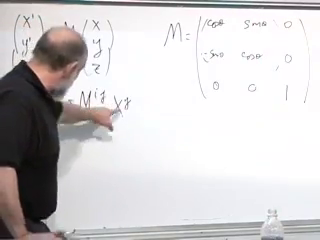
\includegraphics[width=0.82\textwidth]{lecture_05_figure_03.png}
\caption{Die räumliche Drehung, dargestellt sowohl als Matrixgleichung als auch in Indexnotation.}
\lectureframe{01:00:40}
\end{figure}

\section{Lorentz-Matrizen und zusammengesetzte Geschwindigkeiten}

Für eine Bewegung entlang \(x\) lautet die Lorentz-Transformation in Einheiten mit \(c=1\)
\begin{align}
x'&=\gamma_v(x-vt), & y'&=y,\nonumber\\
z'&=z, & t'&=\gamma_v(t-vx),
\end{align}
Dabei ist
\begin{equation}
\gamma_v=\frac{1}{\sqrt{1-v^2}}.
\end{equation}
Bei der Komponentenreihenfolge \((x,y,z,t)\) ergibt sich
\begin{equation}
\begin{pmatrix}x'\\y'\\z'\\t'\end{pmatrix}
=
\begin{pmatrix}
\gamma_v&0&0&-\gamma_vv\\
0&1&0&0\\
0&0&1&0\\
-\gamma_vv&0&0&\gamma_v
\end{pmatrix}
\begin{pmatrix}x\\y\\z\\t\end{pmatrix}.
\label{eq:l5-lorentz-matrix}
\end{equation}

\begin{figure}[H]
\centering
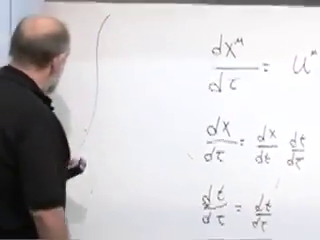
\includegraphics[width=0.82\textwidth]{lecture_05_figure_04.png}
\caption{Die \(4\times4\)-Lorentz-Matrix. Nur die Komponenten \(x\) und \(t\) werden gemischt; \(y\) und \(z\) bleiben unverändert.}
\lectureframe{01:04:40}
\end{figure}

Die Matrixmultiplikation beantwortet nun eine physikalische Frage. Nehmen wir an, ein Beobachter bewegt sich relativ zu uns mit der Geschwindigkeit \(v\), und ein dritter Beobachter bewegt sich relativ zu ihm mit der Geschwindigkeit \(u\), jeweils entlang derselben Achse. Die Newtonsche Kinematik ergäbe \(w=u+v\); damit könnten sich zwei Geschwindigkeiten von jeweils \(3c/4\) zu \(3c/2\) addieren. Die Relativitätstheorie muss eine andere Regel liefern.

Der aktive Teil des Boosts ist die \(2\times2\)-Matrix
\begin{equation}
B(v)=\gamma_v
\begin{pmatrix}1&-v\\-v&1\end{pmatrix}.
\end{equation}
Durch die Zusammensetzung der beiden Boosts ergibt sich
\begin{align}
B(u)B(v)
&=\gamma_u\gamma_v
\begin{pmatrix}1&-u\\-u&1\end{pmatrix}
\begin{pmatrix}1&-v\\-v&1\end{pmatrix}\nonumber\\
&=\gamma_u\gamma_v
\begin{pmatrix}
1+uv&-(u+v)\\
-(u+v)&1+uv
\end{pmatrix}.
\label{eq:l5-composed-boost}
\end{align}
Das Verhältnis eines Nebendiagonaleintrags zu einem Diagonaleintrag bestimmt die Geschwindigkeit des resultierenden Boosts:
\begin{equation}
w=\frac{u+v}{1+uv}
\qquad(c=1).
\end{equation}
Mit wiederhergestellten Einheiten lautet die Beziehung
\begin{equation}
w=\frac{u+v}{1+uv/c^2}.
\label{eq:l5-velocity-addition}
\end{equation}

\begin{figure}[H]
\centering
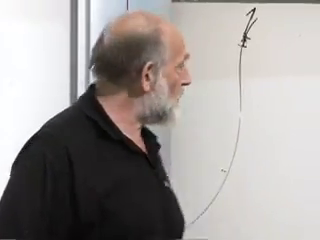
\includegraphics[width=0.82\textwidth]{lecture_05_figure_05.png}
\caption{Die Matrix des zusammengesetzten Boosts und die Geschwindigkeit \(w=(u+v)/(1+uv)\) in natürlichen Einheiten.}
\lectureframe{01:15:35}
\end{figure}

Sind \(u\) und \(v\) jeweils nahe an \(c\), nähert sich der Zähler \(2c\), während sich der Nenner \(2\) nähert. Somit nähert sich \(w\) dem Wert \(c\) und nicht \(2c\). Allgemeiner bildet Gl.~\eqref{eq:l5-velocity-addition} unterluminale Eingangsgeschwindigkeiten auf ein unterluminales Ergebnis ab. Die Matrixmultiplikation berücksichtigt die Geschwindigkeitsgrenze automatisch.

\section{Vierervektoren und das Versagen der gewöhnlichen Geschwindigkeit}

Ein Vierervektor ist ein beliebiges Objekt, dessen vier Komponenten sich bei Drehungen und Lorentz-Boosts genauso transformieren wie die Raum-Zeit-Koordinaten. Ist \(V^\mu\) ein Vierervektor, so gilt bei unserer Vorzeichenkonvention
\begin{equation}
V_\mu=(-V^1,-V^2,-V^3,V^0),
\end{equation}
und für seine invariante Norm
\begin{equation}
V_\mu V^\mu=(V^0)^2-(V^1)^2-(V^2)^2-(V^3)^2.
\end{equation}
Auch für zwei Vierervektoren \(V^\mu\) und \(W^\mu\) ist die Kontraktion
\begin{equation}
W_\mu V^\mu
=W^0V^0-W^1V^1-W^2V^2-W^3V^3
\end{equation}
invariant. Die Komponenten ändern sich beim Übergang zwischen Bezugssystemen; die Kontraktion bleibt unverändert.

Die gewöhnliche Geschwindigkeit hat nur drei Komponenten:
\begin{equation}
\mathbf v=\left(\frac{dx}{dt},\frac{dy}{dt},\frac{dz}{dt}\right).
\end{equation}
Das Anhängen von \(dt/dt=1\) macht sie noch nicht zu einem brauchbaren Vierervektor. Die vierte Komponente wäre trivial, und das so entstehende Objekt würde sich unter Lorentz-Transformationen nicht linear transformieren. Die Koordinatenzeit \(t\) ändert sich von einem Bezugssystem zum anderen; die Ableitung nach \(t\) zerstört daher das gewünschte Transformationsgesetz.

Die Eigenzeit schafft Abhilfe. Entlang einer Weltlinie definieren wir
\begin{equation}
u^\mu=\frac{dX^\mu}{d\tau}.
\label{eq:l5-four-velocity}
\end{equation}
Das Differential \(dX^\mu\) ist ein Vierervektor und \(d\tau\) invariant, also ist auch ihr Quotient ein Vierervektor. Das Adjektiv ``eigen'' bezieht sich auf die Uhr im Nenner.

Die Kettenregel verknüpft dieses Objekt mit der gewöhnlichen Geschwindigkeit:
\begin{equation}
\frac{dx}{d\tau}=\frac{dx}{dt}\frac{dt}{d\tau},
\end{equation}
Entsprechend gilt dies für \(y\) und \(z\). Aus Gl.~\eqref{eq:l5-proper-time} folgt
\begin{align}
\left(\frac{d\tau}{dt}\right)^2
&=1-\left(\frac{dx}{dt}\right)^2
    -\left(\frac{dy}{dt}\right)^2
    -\left(\frac{dz}{dt}\right)^2\nonumber\\
&=1-v^2
\qquad(c=1),
\end{align}
und damit
\begin{equation}
\frac{dt}{d\tau}=\gamma_v=\frac{1}{\sqrt{1-v^2}}.
\end{equation}
Die vier Komponenten lauten
\begin{equation}
u^i=\gamma_v v^i,
\qquad
u^0=\gamma_v
\qquad(c=1).
\label{eq:l5-four-velocity-components}
\end{equation}
Bei kleinen Geschwindigkeiten gilt \(u^i\simeq v^i\) und \(u^0\simeq1\). Nahe der Lichtgeschwindigkeit wächst \(\gamma_v\) unbegrenzt, und die Eigen-Geschwindigkeit unterscheidet sich deutlich von der gewöhnlichen Geschwindigkeit.

\begin{figure}[H]
\centering
\includegraphics[width=0.82\textwidth]{lecture_05_figure_06.png}
\caption{Die vier Komponenten der Eigen-Geschwindigkeit, ausgedrückt durch die gewöhnliche Geschwindigkeit und den Lorentzfaktor.}
\lectureframe{01:34:40}
\end{figure}

Mit wiederhergestellten üblichen Einheiten und unter Verwendung von \(X^0=ct\) erhält man die Standardform
\begin{equation}
U^\mu=(\gamma_v\mathbf v,\gamma_v c)
\end{equation}
in der hier verwendeten Anordnung mit den räumlichen Komponenten zuerst. Ihre invariante Norm ist
\begin{equation}
U_\mu U^\mu=c^2.
\end{equation}
Somit hat jedes massive Teilchen eine Vierergeschwindigkeit mit demselben invarianten Betrag, obwohl seine räumliche Geschwindigkeit vom Bezugssystem abhängt.

\section{Die Tangente an eine Weltlinie}

Zu Gl.~\eqref{eq:l5-four-velocity} gibt es ein vertrautes euklidisches Analogon. Entlang einer Kurve im gewöhnlichen dreidimensionalen Raum gilt
\begin{equation}
ds^2=dx^2+dy^2+dz^2.
\end{equation}
Die differentielle Verschiebung \((dx,dy,dz)\) zeigt entlang der Kurve, ist aber kein Einheitsvektor. Dividiert man sie durch das Bogenelement, erhält man
\begin{equation}
\mathbf T=
\left(\frac{dx}{ds},\frac{dy}{ds},\frac{dz}{ds}\right),
\qquad
\mathbf T\cdot\mathbf T=1.
\end{equation}
Die relativistische Konstruktion folgt derselben Idee, wobei die Eigenzeit an die Stelle der euklidischen Bogenlänge tritt. Der Vektor \(u^\mu=dX^\mu/d\tau\) ist tangential zur Weltlinie.

\begin{figure}[H]
\centering
\includegraphics[width=0.82\textwidth]{lecture_05_figure_07.png}
\caption{Die euklidische Konstruktion eines Tangentialvektors: Die differentielle Verschiebung wird durch das Bogenelement \(ds\) dividiert. Entlang einer zeitartigen Weltlinie übernimmt die Eigenzeit die entsprechende Rolle.}
\lectureframe{01:39:30}
\end{figure}

\begin{classroomqa}
\audiencequestion{Sind Eigenzeit und Eigenlänge dasselbe, wenn \(c=1\) gilt?}
\lecturerresponse{Die Festlegung \(c=1\) setzt Zeit und Strecke in dieselben Einheiten; sie hebt die Minuszeichen der Raum-Zeit-Geometrie nicht auf. Im euklidischen Analogon ist \(s\) die gewöhnliche, entlang einer räumlichen Kurve gemessene Strecke. Entlang einer zeitartigen Weltlinie ist \(\tau\) die von einer Uhr gemessene verstrichene Zeit. Die Konstruktionen sind analog, aber die Geometrien sind verschieden.}
\end{classroomqa}

Durch nochmaliges Ableiten definieren wir die Eigenbeschleunigung:
\begin{equation}
a^\mu=\frac{du^\mu}{d\tau}.
\end{equation}
Diese Größe muss an die Stelle von \(d^2\mathbf x/dt^2\) treten, wenn man das zweite Newtonsche Gesetz relativistisch formuliert. Da \(u_\mu u^\mu\) konstant ist, gilt
\begin{equation}
\frac{d}{d\tau}(u_\mu u^\mu)=2u_\mu a^\mu=0,
\end{equation}
Die Viererbeschleunigung steht also Minkowski-orthogonal zur Vierergeschwindigkeit.\editorialnote{Die Orthogonalität folgt unmittelbar aus der invarianten Norm und ist hier als nächste mathematische Folgerung aus der Definition aufgenommen.}

\section{Viererimpuls und Energie}

Der Impuls ist unser letztes Beispiel, weil er bei Kollisionen und Zerfällen erhalten bleibt. Das Teilchen hat eine feste intrinsische Masse \(m\), die oft Ruhemasse genannt wird. Sie ändert sich nicht mit der Geschwindigkeit. Der relativistische Impuls ist diese feste Masse multipliziert mit der Vierergeschwindigkeit:
\begin{equation}
p^\mu=mu^\mu.
\label{eq:l5-four-momentum}
\end{equation}
In Einheiten mit \(c=1\) gilt
\begin{equation}
p^i=\gamma_v m v^i,
\qquad
p^0=\gamma_v m.
\end{equation}
Bei kleinen Geschwindigkeiten gilt \(\gamma_v\simeq1\), sodass die räumlichen Komponenten zum Newtonschen Impuls \(m\mathbf v\) werden. Bei hohen Geschwindigkeiten wachsen sie schneller als \(m\mathbf v\).

Die Zeitkomponente ist die Energie. In den üblichen Einheiten und mit \(X^0=ct\) gilt
\begin{equation}
P^\mu=(\mathbf p,E/c)
=(\gamma_v m\mathbf v,\gamma_v mc),
\end{equation}
und damit
\begin{equation}
E=\gamma_v mc^2
=mc^2\left(1-\frac{v^2}{c^2}\right)^{-1/2}.
\label{eq:l5-relativistic-energy}
\end{equation}

Um die gewöhnliche Mechanik wiederzugewinnen, setzen wir
\(\epsilon=v^2/c^2\ll1\). Die Binomialentwicklung ergibt
\begin{equation}
(1-\epsilon)^p=1-p\epsilon+O(\epsilon^2).
\end{equation}
Mit \(p=-1/2\) folgt
\begin{align}
E
&=mc^2\left(1-\frac{v^2}{c^2}\right)^{-1/2}\nonumber\\
&=mc^2\left[1+\frac12\frac{v^2}{c^2}
  +O\!\left(\frac{v^4}{c^4}\right)\right]\nonumber\\
&=mc^2+\frac12mv^2+O\!\left(\frac{mv^4}{c^2}\right).
\label{eq:l5-energy-expansion}
\end{align}

\begin{figure}[H]
\centering
\includegraphics[width=0.82\textwidth]{lecture_05_figure_08.png}
\caption{Die Entwicklung der relativistischen Energie bei kleinen Geschwindigkeiten zeigt die Ruheenergie und die Newtonsche kinetische Energie.}
\lectureframe{01:51:30}
\end{figure}

Der erste Term, \(mc^2\), ist auch in Ruhe vorhanden. In einem Newtonschen Problem mit einer festen Teilchenmenge und unveränderten Massen addiert dieser Term vor und nach der Bewegung dieselbe Konstante, sodass bei der üblichen Bilanzierung nur \(\tfrac12mv^2\) eine Rolle spielt. Die Relativitätstheorie zeigt, dass die weggelassene Konstante die ganze Zeit physikalische Energie war.

Energie und Impuls sind also keine voneinander unabhängigen Erhaltungsgrößen. Sie sind die vier Komponenten eines einzigen erhaltenen Vektors. Ein Lorentz-Boost mischt sie: Was ein Beobachter als Energie bezeichnet, trägt für einen anderen Beobachter teilweise zum Impuls bei, und umgekehrt. Dennoch ist der Gesamtviererimpuls eines isolierten Systems vor und nach jeder Kollision oder jedem Zerfall in jedem Inertialsystem derselbe.

Damit erreichen wir die Schwelle zur relativistischen Mechanik. Als Nächstes gilt es, die Kraft mithilfe der Eigenbeschleunigung auszudrücken und relativistische Wellengleichungen zu verstehen, insbesondere die Gleichungen für Elektromagnetismus und Licht.
\chapter{Invariante Gesetze, Vierervektoren und der Feldstärketensor}

Wir beginnen mit einem Gesetz, dem die Natur hätte folgen können, es aber nicht tut. Sein Scheitern zeigt uns, wie ein physikalisches Gesetz formuliert werden sollte. Derselbe Test führt zunächst von Koordinatenkomponenten zu gewöhnlichen Vektoren, dann von gewöhnlichen Vektoren zu Vierervektoren und schließlich von Vierervektoren zu Tensoren. Am Ende sind elektrische und magnetische Felder keine getrennten Objekte mehr: Zusammen belegen sie die sechs unabhängigen Komponenten eines antisymmetrischen Tensors.

Sofern nichts anderes angegeben ist, verwenden wir Einheiten, in denen \(c=1\) gilt, ordnen die Raumzeitkomponenten als \((1,2,3,0)=(x,y,z,t)\) an und verwenden die Metriksignatur \((-,-,-,+)\).

\section{Ein mögliches Gesetz mit der falschen Symmetrie}

Wir legen eine \(x\)- und eine \(y\)-Achse fest im Raum fest. Nun legen wir fest, dass zwei Teilchen wechselwirken, sobald ihre \(x\)-Koordinaten übereinstimmen. Die Wechselwirkung könnte ihre Bewegung umkehren oder sie in neue Richtungen treiben; auf die genaue Dynamik kommt es nicht an. Auslöser soll schlicht die Bedingung \begin{equation}
  x_1-x_2=0,
\end{equation} sein, wobei die Indizes Teilchen und nicht Koordinatenkomponenten bezeichnen. Diese Regel ist mathematisch widerspruchsfrei. Die Frage ist, was sie physikalisch unplausibel macht.

\begin{classroomqa}
\audiencequestion{Verletzt die Regel die Homogenität des Raums?}
\lecturerresponse{Nein. Eine Verschiebung des Ursprungs ändert beide Koordinaten um denselben Betrag und lässt \(x_1-x_2\) unverändert. Die Regel zeichnet keinen bestimmten Ort aus. Ihr Mangel liegt in der Isotropie: Sie zeichnet eine bestimmte Richtung aus.}
\end{classroomqa}

Drehen wir die Achsen um \(90^\circ\). Die bisherige \(x\)-Richtung heißt nun \(y\), sodass dieselben physikalischen Ereignisse durch die Gleichheit der \(y\)-Koordinaten beschrieben würden. Bei einem beliebigen Drehwinkel hinge die Bedingung von einer Linearkombination aus \(x\) und \(y\) ab. Die Form des Gesetzes hängt also davon ab, wie die Tafel ausgerichtet ist. Es ist translationsinvariant, aber nicht rotationsinvariant.

Physikalische Gesetze formulieren wir gewöhnlich in orthogonalen Koordinaten möglichst einfach. Man kann auch allgemeinere Koordinaten verwenden, doch dann werden die Metrik und die Formeln komplizierter. Innerhalb der Klasse orthogonaler kartesischer Bezugssysteme darf keine Ausrichtung ausgezeichnet sein.

Die Korrektur ist unmittelbar klar. In zwei Dimensionen müssen beide Koordinaten übereinstimmen, in drei Dimensionen alle drei: \begin{equation}
  x_1=x_2,
  \qquad y_1=y_2,
  \qquad z_1=z_2.
\end{equation} Dann können die Teilchen nur wechselwirken, wenn sie denselben Punkt erreichen, selbst wenn sie sich auf unterschiedlichen Geraden nähern.

\begin{classroomqa}
\audiencequestion{Müssen auch die \(z\)-Koordinaten und die Zeiten übereinstimmen?}
\lecturerresponse{Im dreidimensionalen Raum müssen auch die \(z\)-Koordinaten übereinstimmen. Die Zeit lassen wir vorerst außer Betracht; sobald die räumliche Argumentation abgeschlossen ist, beziehen wir sie wieder ein.}
\end{classroomqa}

Sei \(\boldsymbol r_a\) die Position des Teilchens \(a\). Die drei Komponentenbedingungen lassen sich zu einer Vektorgleichung zusammenfassen: \begin{equation}
  \boldsymbol r_1-\boldsymbol r_2=\boldsymbol 0.
\end{equation} Eine Komponente kann in einem gedrehten Bezugssystem verschwinden, in einem anderen jedoch nicht. Beim gesamten Vektor ist das anders: Sind in einem Bezugssystem alle Komponenten null, so sind sie es in jedem gedrehten Bezugssystem. Ebenso bleiben zwei Vektoren gleich, wenn sie in einem Bezugssystem gleich sind und beide transformiert werden.

\begin{figure}[H]\centering
\includegraphics[width=0.78\textwidth]{lecture_06_figure_01.png}\caption{Die drei Koordinatengleichheiten sorgen dafür, dass eine Kollision räumliches Zusammentreffen bedeutet und nicht das Zusammentreffen entlang einer ausgezeichneten Achse.}\lectureframe{00:09:00}\end{figure}

Darum sind Vektorgleichungen nützlich. Ihre Komponenten ändern sich, aber das Objekt transformiert sich als zusammenhängendes Ganzes. Ein Gesetz, das für das vollständige Objekt formuliert ist, kann seine Form bei einer Drehung der Koordinaten beibehalten.

\section{Zusammentreffen in der Raumzeit}

Ersetzen wir nun die vertikale räumliche Achse durch die Zeit. Ein Newtonsches Gesetz könnte besagen, dass zwei Bewegungsänderungen nur zu gleichen Zeiten stattfinden. In der Newtonschen Mechanik gilt die Gleichzeitigkeit für alle Inertialbeobachter gleichermaßen, daher ist ein solches Gesetz möglich. In der speziellen Relativitätstheorie zeichnet es jedoch ein bevorzugtes Bezugssystem aus. Ereignisse, die in einem Bezugssystem gleichzeitig sind, müssen es in einem anderen nicht sein.

Nur die Gleichheit der räumlichen Koordinaten zu verlangen, ist nicht besser. Eine Raumzeitverschiebung kann verschwindende räumliche Komponenten und zugleich eine von null verschiedene Zeitkomponente haben: \begin{equation}
  \Delta X^\mu=(0,0,0,\Delta t),
\end{equation} Außerdem mischt ein Boost \(\Delta t\) mit einer räumlichen Komponente. Die invariante lokale Aussage lautet, dass die beiden Bewegungsänderungen am selben Ereignis stattfinden. Eine einfache Kollision erfordert daher \begin{equation}
  X_1^\mu=X_2^\mu,
  \qquad\text{or}\qquad
  X_1^\mu-X_2^\mu=0.
\end{equation} Alle vier Koordinaten stimmen überein: Die Teilchen befinden sich zur selben Zeit am selben Ort.

Das Kollisionsbeispiel führt zu einer allgemeinen Regel für die Formulierung physikalischer Gesetze. Wir können alles auf eine Seite bringen und einen vollständigen Vierervektor gleich null setzen oder einen vollständigen Vierervektor einem anderen gleichsetzen. Gleichsetzungen einzelner, nicht zusammengehöriger Komponenten eines Vierervektors sind für sich genommen keine Lorentz-invarianten Aussagen.

\section{Boosts, Drehungen und Matrixschreibweise}

Ein Vierervektor ist ein Objekt, das sich so transformiert wie eine Raumzeitverschiebung. Um diese Definition nutzbar zu machen, betrachten wir zunächst noch einmal die Transformationen der Koordinaten selbst. Für einen Boost mit Geschwindigkeit \(v\) in \(x\)-Richtung gilt: \begin{align}
  x'&=\gamma(x-vt), & y'&=y, & z'&=z,
  & t'&=\gamma(t-vx),                                      \label{eq:l6-boost}
\end{align} Dabei ist \begin{equation}
  \gamma(v)=\frac{1}{\sqrt{1-v^2}}.
\end{equation}

\begin{classroomqa}
\audiencequestion{Wurde in diesen Formeln die Lichtgeschwindigkeit gleich eins gesetzt?}
\lecturerresponse{Ja. Um die Einheiten wieder einzusetzen, setzen wir \(X^0=ct\), ersetzen \(1-v^2\) durch \(1-v^2/c^2\) und ergänzen die entsprechenden Faktoren von \(c\) in den gemischten Raum--Zeit-Termen.}
\end{classroomqa}

Eine Drehung um die \(z\)-Achse mischt \(x\) und \(y\), während \(z\) und \(t\) unverändert bleiben: \begin{equation}
\begin{pmatrix}
  x'\\ y'\\ z'\\ t'
\end{pmatrix}
=
\begin{pmatrix}
  \cos\theta & \sin\theta & 0 & 0\\
  -\sin\theta & \cos\theta & 0 & 0\\
  0 & 0 & 1 & 0\\
  0 & 0 & 0 & 1
\end{pmatrix}
\begin{pmatrix}
  x\\ y\\ z\\ t
\end{pmatrix}.
\end{equation} Die Nullen sollte man ausdrücklich hinschreiben: So ist klar zu erkennen, welche Komponenten in die jeweilige transformierte Koordinate nicht eingehen. In derselben Reihenfolge lautet der Boost aus Gl.~\eqref{eq:l6-boost}: \begin{equation}
\begin{pmatrix}
  x'\\ y'\\ z'\\ t'
\end{pmatrix}
=
\begin{pmatrix}
  \gamma & 0 & 0 & -\gamma v\\
  0 & 1 & 0 & 0\\
  0 & 0 & 1 & 0\\
  -\gamma v & 0 & 0 & \gamma
\end{pmatrix}
\begin{pmatrix}
  x\\ y\\ z\\ t
\end{pmatrix}.
\end{equation}

Drehungen und Boosts lassen sich durch Matrixmultiplikation zusammensetzen. Um einen Boost in eine Richtung auszuführen, die nicht mit der ursprünglichen \(x\)-Achse übereinstimmt, kann man diese Richtung auf die \(x\)-Achse drehen, den Boost anwenden und anschließend nach Bedarf zurückdrehen. Produkte dieser elementaren Matrizen erzeugen allgemeinere Lorentz-Transformationen.

\begin{classroomqa}
\audiencequestion{Spielt es eine Rolle, ob man zuerst dreht und dann boostet oder zuerst boostet und dann dreht?}
\lecturerresponse{Ja. Nach dem ersten Schritt haben sich die Achsen geändert, auf die der zweite Schritt wirkt. Die beiden Matrixprodukte müssen daher nicht übereinstimmen; die Reihenfolge der Operationen ist also entscheidend.}
\end{classroomqa}

Alle diese linearen Transformationen lassen sich zusammenfassend schreiben als \begin{equation}
  X'^{\mu}=\Lambda^{\mu}{}_{\nu}X^{\nu}.                  \label{eq:l6-vector-transform}
\end{equation} Über den wiederholten Index \(\nu\) wird summiert, und zwar über \(1,2,3,0\). Das ist die gewöhnliche Zeile-mal-Spalte-Summe der Matrixmultiplikation, in Indexschreibweise ausgedrückt.

\begin{figure}[H]\centering
\includegraphics[width=0.78\textwidth]{lecture_06_figure_02.png}\caption{Die indizierte Lorentz-Transformation über ihrer Darstellung in Spaltenvektorform.}\lectureframe{00:31:55}\end{figure}

Gl.~\eqref{eq:l6-vector-transform} ist zugleich die Definition eines allgemeinen kontravarianten Vierervektors. Ist \(A^\mu\) ein solcher Vektor, dann gilt \begin{equation}
  A'^{\mu}=\Lambda^{\mu}{}_{\nu}A^{\nu}.
\end{equation} Seine vier Komponenten müssen keine Position beschreiben. Entscheidend für die Bezeichnung als Vierervektor ist sein Transformationsgesetz.

\section{Skalare, die Metrik und invariante Produkte}

Bevor wir weitere Vierervektoren verwenden, lohnt es sich, zum einfacheren Begriff des Skalars zurückzukehren. Bei räumlichen Drehungen ist die Temperatur an einem bestimmten Punkt ein Skalar, ebenso der Abstand zwischen zwei bestimmten Punkten. Beide Größen sind jeweils eine Zahl, die nicht von der Ausrichtung der Achsen abhängt. Man könnte sogar die bewusst unsinnige Zahlenbehauptung aufstellen, ein in Zentimetern gemessener Abstand sei gleich der in Grad Fahrenheit gemessenen Raumtemperatur. Die Behauptung hat keine physikalische Aussagekraft, aber da beide Seiten Rotationsskalare sind, hängt ihre Wahrheit oder Falschheit nicht davon ab, wie die Achsen gedreht werden.

Vektorkomponenten sind keine Skalare. Wir brauchen daher eine systematische Methode, sie zu Skalaren zusammenzufassen. Schreiben wir einen allgemeinen kontravarianten Vierervektor als \begin{equation}
  A^\mu=(A^1,A^2,A^3,A^0).
\end{equation} Die kovarianten Komponenten beschreiben dasselbe geometrische Objekt mit einem unteren Index. Bei unserer Signatur erhält man sie mithilfe der Minkowski-Metrik: \begin{equation}
  A_\mu=\eta_{\mu\nu}A^\nu,
  \qquad
  \eta_{\mu\nu}=
  \begin{pmatrix}
    -1&0&0&0\\
    0&-1&0&0\\
    0&0&-1&0\\
    0&0&0&1
  \end{pmatrix},                                          \label{eq:l6-metric}
\end{equation} Somit gilt \begin{equation}
  A_\mu=(-A^1,-A^2,-A^3,A^0).
\end{equation}

\begin{classroomqa}
\audiencequestion{Sind auf der Tafel bei zwei Indizes die Vorzeichen falsch?}
\lecturerresponse{Ja. In der dargestellten Spalte braucht die räumliche Komponente das entsprechende Minuszeichen; außerdem müssen die Komponenten rechts in der Indexsenkungsgleichung vor der Multiplikation mit \(\eta_{\mu\nu}\) obere Indizes tragen. Der Zeitindex ist \(0\), nicht \(4\).}
\end{classroomqa}

\begin{figure}[H]\centering
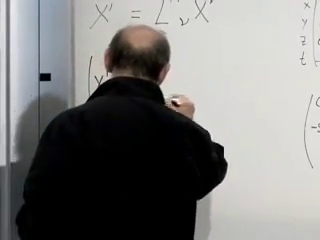
\includegraphics[width=0.8\textwidth]{lecture_06_figure_03.png}\caption{Kontravariante und kovariante Komponenten, die Metrikmatrix und der Beginn der invarianten Kontraktion.}\lectureframe{00:45:00}\end{figure}

Das Senken eines Index ist keine bloße Schreibkonvention. Es berücksichtigt die Vorzeichen, die für die Lorentz-invariante Norm erforderlich sind: \begin{align}
  A_\mu A^\mu
  &=-(A^1)^2-(A^2)^2-(A^3)^2+(A^0)^2,                    \label{eq:l6-norm}\\
  X_\mu X^\mu
  &=t^2-x^2-y^2-z^2.
\end{align} Der zweite Ausdruck ist das invariante Raumzeitintervall vom Ursprung aus. Da \(A^\mu\) sich genauso transformiert wie \(X^\mu\), ist auch ihre Kontraktion invariant.

Die Notation macht zudem eine nützliche Buchführungsregel deutlich: Ein wiederholter Summationsindex tritt einmal oben und einmal unten auf. Zum Beispiel gilt \begin{equation}
  A_\mu A^\mu
  =\eta_{\mu\nu}A^\mu A^\nu.
\end{equation} Die Namen der summierten, sogenannten stummen Indizes können geändert werden, ohne dass sich die Größe ändert.

\begin{classroomqa}
\audiencequestion{Sollte man einen dieser Vektoren als Zeile und den anderen als Spalte auffassen, und spielt ihre Reihenfolge eine Rolle?}
\lecturerresponse{Für die vorliegende Rechnung betrachten wir die indizierten Größen als Komponenten und lassen die Metrik die Kontraktion ausführen; wir brauchen die Diskussion nicht in eine Operatoralgebra mit Zeilen und Spalten umzudeuten. Es handelt sich um gewöhnliche Zahlen, deren Reihenfolge keine Rolle spielt. Bei nichtvertauschenden Operatoren wäre mehr Sorgfalt nötig, doch darum geht es hier nicht.}
\end{classroomqa}

Dieselbe Konstruktion liefert ein inneres Produkt zweier verschiedener Vierervektoren: \begin{equation}
  A\mathbin{\cdot}B=A_\mu B^\mu=A^\mu B_\mu.
\end{equation} Seine Invarianz lässt sich zeigen, ohne eine Lorentz-Matrix explizit hinzuschreiben. Da \(A+B\) und \(A-B\) Vierervektoren sind, sind ihre beiden quadrierten Normen invariant: \begin{align}
  (A+B)^2&=A^2+B^2+2A\mathbin{\cdot}B,\\
  (A-B)^2&=A^2+B^2-2A\mathbin{\cdot}B.
\end{align} Durch Subtraktion erhält man \begin{equation}
  (A+B)^2-(A-B)^2=4A\mathbin{\cdot}B,                    \label{eq:l6-polarization}
\end{equation} und somit ist auch \(A\mathbin{\cdot}B\) invariant. Der Faktor vier ergibt sich unmittelbar aus der Entwicklung.\editorialnote{Das Argument an der Tafel liefert diese Polarisationsidentität; durch die Angabe des Faktors wird die mündlich erläuterte Kürzung eindeutig.}

\begin{figure}[H]\centering
\includegraphics[width=0.8\textwidth]{lecture_06_figure_04.png}\caption{Die beiden invarianten Quadrate, mit denen das innere Produkt verschiedener Vierervektoren isoliert wird.}\lectureframe{00:52:20}\end{figure}

Invariante Größen sind naheliegende Bestandteile physikalischer Gesetze: Anders als eine einzelne Komponente behalten sie ihren Wert beim Wechsel des Bezugssystems bei.

\section{Eigenzeitgeschwindigkeit und Viererimpuls}

Betrachten wir zwei benachbarte Ereignisse auf der Weltlinie eines Teilchens. Ihre Differenz ist der infinitesimale Vierervektor \begin{equation}
  dX^\mu=(dx,dy,dz,dt).
\end{equation} Für eine zeitartige Weltlinie ist die Eigenzeit definiert durch \begin{equation}
  d\tau^2=dX_\mu dX^\mu
  =dt^2-dx^2-dy^2-dz^2.                                  \label{eq:l6-proper-time}
\end{equation} Die Eigenzeitgeschwindigkeit ist \begin{equation}
  U^\mu=\frac{dX^\mu}{d\tau}.                            \label{eq:l6-four-velocity}
\end{equation} Sie beschreibt die Änderungsrate der Raumzeitposition bezüglich der Eigenzeit des Teilchens, nicht bezüglich der Koordinatenzeit eines gewählten Bezugssystems.

Obwohl \(U^\mu\) vier Komponenten hat, sind nur drei davon unabhängig. Teilen wir Gl.~\eqref{eq:l6-proper-time} durch \(d\tau^2\), so erhalten wir \begin{equation}
  U_\mu U^\mu=1.
\end{equation} Damit ist die Vierergeschwindigkeit ein zeitartiger Einheitsvektor. Die Wahl der Zukunftsrichtung legt das Vorzeichen ihrer Zeitkomponente fest.

\begin{classroomqa}
\audiencequestion{Geht die Vierergeschwindigkeit bei Geschwindigkeiten weit unter \(c\) in die gewöhnliche Geschwindigkeit über?}
\lecturerresponse{Ihre drei räumlichen Komponenten nähern sich der gewöhnlichen Geschwindigkeit an, während ihre Zeitkomponente in Einheiten mit \(c=1\) gegen eins geht. Der Zusammenhang folgt, wenn man die Kettenregel anwendet und \(dt/d\tau\) berechnet.}
\end{classroomqa}

Für jede räumliche Komponente gilt \begin{equation}
  U^i=\frac{dx^i}{d\tau}
     =\frac{dx^i}{dt}\frac{dt}{d\tau}
     =v^i\frac{dt}{d\tau}.
\end{equation} Teilen wir Gl.~\eqref{eq:l6-proper-time} durch \(dt^2\), so folgt \begin{equation}
  \left(\frac{d\tau}{dt}\right)^2
  =1-v_x^2-v_y^2-v_z^2
  =1-\boldsymbol v^2.
\end{equation} Also gilt \begin{equation}
  \frac{dt}{d\tau}=\frac{1}{\sqrt{1-\boldsymbol v^2}}
  =\gamma(\lvert\boldsymbol v\rvert),
\end{equation} und \begin{equation}
  U^\mu=(\gamma v_x,\gamma v_y,\gamma v_z,\gamma).
                                                                  \label{eq:l6-u-components}
\end{equation}

\begin{figure}[H]\centering
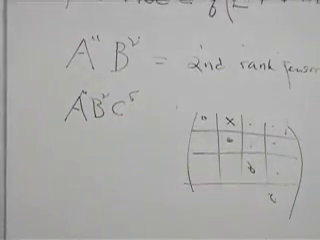
\includegraphics[width=0.8\textwidth]{lecture_06_figure_05.png}\caption{Die Eigenzeitrechnung, aus der \(dt/d\tau=\gamma\) folgt und die die Eigenzeitgeschwindigkeit mit der gewöhnlichen Geschwindigkeit verknüpft.}\lectureframe{01:02:00}\end{figure}

\begin{classroomqa}
\audiencequestion{Bedeutet \(dx^2/dt^2\) eine zweite Ableitung, und entstehen beim Quadrieren eines Vektors nicht gemischte Terme?}
\lecturerresponse{Hier bedeutet es \((dx/dt)^2\), also das Quadrat einer ersten Ableitung. Außerdem steht \(\boldsymbol v^2\) für das euklidische Skalarprodukt \(v_x^2+v_y^2+v_z^2\), nicht für das Quadrat der formalen Summe \(v_x+v_y+v_z\); gemischte Terme treten nicht auf.}
\end{classroomqa}

\begin{classroomqa}
\audiencequestion{Ist das \(v\) in \(\gamma(v)\) die Relativgeschwindigkeit zweier Bezugssysteme oder die Geschwindigkeit des Teilchens?}
\lecturerresponse{Hier ist die Geschwindigkeit des Teilchens im gewählten Bezugssystem gemeint. Die Funktion \(\gamma(v)=1/\sqrt{1-v^2}\) lässt sich für jede Geschwindigkeit auswerten: Bei einem Boost wertet man sie bei der Relativgeschwindigkeit der Bezugssysteme aus, bei der Vierergeschwindigkeit bei der Teilchengeschwindigkeit.}
\end{classroomqa}

Für \(v\ll1\) gilt \(\gamma\simeq1\); die räumlichen Komponenten von \(U^\mu\) nähern sich also \(\boldsymbol v\), und \(U^0\) nähert sich eins. Nähert sich die gewöhnliche Geschwindigkeit der Lichtgeschwindigkeit, so wächst \(\gamma\) und damit wachsen auch alle von null verschiedenen Komponenten der Vierergeschwindigkeit unbegrenzt.

\begin{classroomqa}
\audiencequestion{Müsste \(U^0\) nicht die Einheit einer Geschwindigkeit haben, statt nahe bei der Zahl eins zu liegen?}
\lecturerresponse{Die Einheiten sind weggefallen, weil \(c\) gleich eins gesetzt wurde. Für \(X^0=ct\) gilt \(U^\mu=(\gamma\boldsymbol v,\gamma c)\); die Zeitkomponente nähert sich also \(c\) und \(U_\mu U^\mu=c^2\).}
\end{classroomqa}

Für ein Teilchen mit Ruhemasse \(m\) definieren wir den Viererimpuls durch \begin{equation}
  P^\mu=mU^\mu.
\end{equation} In natürlichen Einheiten gilt \begin{equation}
  P^\mu=(\gamma m\boldsymbol v,\gamma m).
\end{equation} Bei kleinen Geschwindigkeiten nähern sich die ersten drei Komponenten dem Newtonschen Impuls \(m\boldsymbol v\). Setzen wir die Einheiten wieder ein, erhalten wir \begin{equation}
  P^\mu=(\gamma m\boldsymbol v,E/c),
  \qquad E=\gamma mc^2,
\end{equation} und damit \begin{equation}
  E=mc^2+\frac{1}{2}m\boldsymbol v^2+O(mv^4/c^2).
\end{equation} Die Zeitkomponente ist in Einheiten mit \(c=1\) die Energie oder, wenn allen vier Komponenten Impulseinheiten zugewiesen werden, die Energie dividiert durch \(c\).

\begin{classroomqa}
\audiencequestion{Ist die gewöhnliche Geschwindigkeit \(\boldsymbol v\) mit einer angehängten vierten Komponente selbst ein Vierervektor?}
\lecturerresponse{Nein. Die gewöhnliche Dreiergeschwindigkeit transformiert sich nicht wie ein Vierervektor. Der Faktor \(\gamma\) und die Definition über die Eigenzeit sind wesentlich; der Vierervektor ist \(U^\mu\), nicht \(\boldsymbol v\).}
\end{classroomqa}

\section{Warum sich elektrische und magnetische Felder mischen müssen}

Nun machen wir einen kurzen Abstecher von der Relativitätstheorie. Wir beginnen mit der Bewegungsgleichung aus der Zeit vor Einstein und fragen, wie sie umformuliert werden muss, damit sie in jedem Inertialsystem gilt. Die gewöhnliche Beschleunigung ist die Zeitableitung der gewöhnlichen Geschwindigkeit. Ihr vierdimensionales Analogon ist naheliegenderweise \begin{equation}
  A^\mu=\frac{dU^\mu}{d\tau}.
\end{equation} Die räumlichen Komponenten nähern sich bei kleinen Geschwindigkeiten der gewöhnlichen Beschleunigung an. Die vollständige relativistische Bewegungsgleichung stellen wir zurück; zunächst betrachten wir das alte Kraftgesetz.

Für eine Ladung \(q\) in elektrischen und magnetischen Feldern gilt \begin{equation}
  \boldsymbol F=m\boldsymbol a
  =q\left(\boldsymbol E+\boldsymbol v\times\boldsymbol B\right).
                                                                  \label{eq:l6-lorentz-force}
\end{equation} Der elektrische Term hängt nicht von der Teilchengeschwindigkeit ab, der magnetische dagegen schon.

\begin{figure}[H]\centering
\includegraphics[width=0.8\textwidth]{lecture_06_figure_06.png}\caption{Die vorrelativistische Form des Lorentz-Kraftgesetzes, die zur Zusammenfassung von \(\boldsymbol E\) und \(\boldsymbol B\) motiviert.}\lectureframe{01:18:20}\end{figure}

Angenommen, ein Beobachter sieht kein elektrisches Feld, wohl aber ein Magnetfeld und eine bewegte Ladung. Auf die Ladung wirkt eine magnetische Kraft. Im momentanen Ruhesystem der Ladung gilt jedoch \(\boldsymbol v=0\), sodass der magnetische Term in Gl.~\eqref{eq:l6-lorentz-force} verschwindet. Die physikalische Weltlinie wird nicht dadurch inertial, dass sich die Koordinaten ändern; die Kraft im neuen Bezugssystem muss daher einen elektrischen Beitrag enthalten. Genauer gesagt lässt sich eine von null verschiedene Viererbeschleunigung durch einen Wechsel des Inertialsystems nicht in null überführen, auch wenn die Dreierbeschleunigung und ihre Komponenten transformiert werden.\editorialnote{Diese Aussage über die Viererbeschleunigung ist die invariante Form des Arguments aus der Vorlesung und vermeidet es, die gewöhnliche Dreierbeschleunigung selbst als bezugssysteminvariant zu behandeln.}

Elektrische und magnetische Felder müssen sich folglich ineinander transformieren. Zusammen haben sie sechs Komponenten und bilden daher weder einen einzelnen Skalar noch einen Vierervektor. Wir benötigen ein neues Transformationsobjekt.

\section{Tensoren: eine Transformation für jeden Index}

Ein Skalar lässt sich als Tensor nullter Stufe bezeichnen; er hat keine Indizes. Ein Vierervektor ist ein Tensor erster Stufe mit einem Index, der vier mögliche Werte annimmt. Das einfachste Beispiel für einen Tensor zweiter Stufe ist ein Produkt \begin{equation}
  A^\mu B^\nu.
\end{equation} Jeder Index kann vier Werte annehmen; das Objekt hat also \(4^2=16\) Komponenten und lässt sich als Array der Größe \(4\times4\) darstellen. Das Produkt dreier Vektoren \begin{equation}
  A^\mu B^\nu C^\sigma,
\end{equation} hat \(4^3=64\) Komponenten und ist ein Tensor dritter Stufe. Bei höheren Stufen setzt sich das Muster fort. Wichtiger als der Name ist die Regel, die das Objekt definiert.

Wenn \begin{equation}
  A'^{\mu}=\Lambda^\mu{}_{\nu}A^\nu,
  \qquad
  B'^{\sigma}=\Lambda^\sigma{}_{\tau}B^\tau,
\end{equation} gilt, transformiert sich ihr Produkt gemäß \begin{equation}
  A'^{\mu}B'^{\sigma}
  =\Lambda^\mu{}_{\nu}\Lambda^\sigma{}_{\tau}
   A^\nu B^\tau.
\end{equation} Daraus ergibt sich das definierende Transformationsgesetz für einen kontravarianten Tensor zweiter Stufe: \begin{equation}
  T'^{\mu\sigma}
  =\Lambda^\mu{}_{\nu}\Lambda^\sigma{}_{\tau}T^{\nu\tau}.
                                                                  \label{eq:l6-tensor-transform}
\end{equation} Für jeden Index gibt es eine Lorentz-Matrix. Über die wiederholten Indizes \(\nu\) und \(\tau\) wird summiert; die freien Indizes \(\mu\) und \(\sigma\) bezeichnen die im gestrichenen Bezugssystem berechnete Komponente.

\begin{figure}[H]\centering
\includegraphics[width=0.82\textwidth]{lecture_06_figure_07.png}\caption{Die Transformation zweier Vektoren und das daraus folgende Transformationsgesetz mit zwei Matrizen für einen Tensor zweiter Stufe.}\lectureframe{01:27:15}\end{figure}

Ein Tensor muss nicht das Produkt einzelner Vektoren sein. Sowohl \(A^\mu B^\nu\) als auch \(A^\nu B^\mu\) gehorchen dem Tensor-Transformationsgesetz, ebenso ihre Summe und jede Summe der Form \begin{equation}
  A^\mu B^\nu+C^\mu D^\nu.
\end{equation} Die Definition ist das Transformationsgesetz, nicht eine bestimmte Produktdarstellung. Ein Tensor dritter Stufe erhält eine dritte Lorentz-Matrix und so weiter.

\section{Symmetrische und antisymmetrische Tensoren}

Zwei Klassen von Tensoren zweiter Stufe werden besonders nützlich sein. Ein symmetrischer Tensor erfüllt \begin{equation}
  T^{\mu\nu}=T^{\nu\mu},
\end{equation}, sodass spiegelbildlich zur Diagonalen liegende Einträge übereinstimmen. Seine vier Diagonaleinträge und die sechs Einträge auf einer Seite der Diagonalen bestimmen alle übrigen. Damit hat er \begin{equation}
  4+6=10
\end{equation} unabhängige Komponenten.

Ein antisymmetrischer Tensor erfüllt \begin{equation}
  T^{\mu\nu}=-T^{\nu\mu}.                                \label{eq:l6-antisymmetry}
\end{equation} Setzen wir \(\mu=\nu\) in Gl.~\eqref{eq:l6-antisymmetry} ein, erhalten wir \(T^{\mu\mu}=-T^{\mu\mu}\); daher verschwinden alle Diagonaleinträge. Die sechs Einträge in einer Dreieckshälfte bestimmen die anderen sechs mit umgekehrtem Vorzeichen. Es gibt somit genau sechs unabhängige Komponenten.

\begin{figure}[H]\centering
\includegraphics[width=0.82\textwidth]{lecture_06_figure_08.png}\caption{Ein ausgefülltes antisymmetrisches Array der Größe \(4\times4\): Nullen auf der Diagonalen und entgegengesetzte Vorzeichen auf beiden Seiten.}\lectureframe{01:34:25}\end{figure}

Diese Anzahl ist der entscheidende Hinweis. Die drei elektrischen und die drei magnetischen Komponenten lassen sich in einem einzigen antisymmetrischen Tensor zweiter Stufe zusammenfassen.

\section{Der elektromagnetische Feldstärketensor}

Wir ordnen die Raumzeitindizes in Zeilen und Spalten der Reihenfolge \((1,2,3,0)=(x,y,z,t)\) entsprechend an. Die Darstellung an der Tafel lautet \begin{equation}
  F_{\mu\nu}=
  \begin{pmatrix}
    0    & -B_3 & B_2  & E_1\\
    B_3  & 0    & -B_1 & E_2\\
    -B_2 & B_1  & 0    & E_3\\
    -E_1 & -E_2 & -E_3 & 0
  \end{pmatrix}.                                         \label{eq:l6-field-tensor}
\end{equation} Die rein räumlichen Komponenten enthalten das Magnetfeld; die Komponenten mit einem räumlichen und einem Zeitindex enthalten das elektrische Feld. Wegen der Antisymmetrie ergeben sich die Einträge unterhalb der Diagonalen aus den Einträgen oberhalb der Diagonalen.

\begin{classroomqa}
\audiencequestion{Sind die magnetischen Einträge alle negativ, und entsprechen die Indizes \(x,y,z\)?}
\lecturerresponse{Die Vorzeichen im oberen räumlichen Dreieck wechseln wie dargestellt: \(-B_3,+B_2,-B_1\) Die Indizes \(1,2,3\) entsprechen \(x,y,z\), während \(0\) die Zeit bezeichnet. Die Spiegelung an der Diagonalen kehrt jedes Vorzeichen um.}
\end{classroomqa}

\begin{figure}[H]\centering
\includegraphics[width=0.82\textwidth]{lecture_06_figure_09.png}\caption{Der vollständige elektromagnetische Feldstärketensor in der Vorlesung verwendeten Anordnung mit den räumlichen Komponenten zuerst.}\lectureframe{01:41:05}\end{figure}

Üblicherweise schreibt man \(F_{\mu\nu}\) statt eines allgemeinen \(T_{\mu\nu}\). Der Dozent vermutet, der Buchstabe könne auf Faraday verweisen, sagt aber ausdrücklich, dass ihm die Geschichte dieser Notation nicht bekannt ist. Entscheidend sind hier die Antisymmetrie und die sechs Feldkomponenten, nicht diese Vermutung über den Buchstaben.

\begin{classroomqa}
\audiencequestion{Stellt jeder Matrixeintrag die Stärke eines Feldes in der angegebenen Koordinatenebene dar?}
\lecturerresponse{Er ist eine Komponente des elektromagnetischen Feldstärketensors. Die Einträge mit einem Zeitindex sind elektrische Komponenten, die räum--räumlichen Einträge codieren magnetische Komponenten.}
\end{classroomqa}

Klammern wir die Zeile und die Spalte mit dem Zeitindex aus. Der verbleibende antisymmetrische \(3\times3\)-Block ist magnetisch. Seine unabhängigen Komponenten kann man sich zyklisch merken: \begin{equation}
  F_{12}=-B_3,
  \qquad F_{23}=-B_1,
  \qquad F_{31}=-B_2.                                   \label{eq:l6-magnetic-cycle}
\end{equation} Geht man von der ersten Beziehung aus, rückt man die Indizes der Reihe nach entlang \(1\to2\to3\to1\) weiter. Äquivalent dazu gilt \begin{equation}
  F_{ij}=-\epsilon_{ijk}B_k,
\end{equation} mit \(\epsilon_{123}=+1\).\editorialnote{Die Levi--Civita-Formel ist die kompakte Standardform der an der Tafel Schritt für Schritt entwickelten zyklischen Regel.}

\begin{figure}[H]\centering
\includegraphics[width=0.82\textwidth]{lecture_06_figure_10.png}\caption{Die zyklischen räumlichen Komponenten, die das Magnetfeld im antisymmetrischen Tensor codieren.}\lectureframe{01:46:20}\end{figure}

Die Zuordnungen für das elektrische Feld sind direkter: \begin{equation}
  E_1=F_{10},
  \qquad E_2=F_{20},
  \qquad E_3=F_{30}.
\end{equation}

Das Magnetfeld hat folglich zwei nützliche Darstellungen. Im dreidimensionalen Raum lässt sich ein axialer Vektor mit drei Komponenten einem antisymmetrischen \(3\times3\)-Tensor zuordnen. In der Raumzeit ist es dagegen nur der räumliche Anteil des sechskomponentigen Tensors \(F_{\mu\nu}\). Diese Zuordnung ist spezifisch für drei Dimensionen: Ein antisymmetrischer \(4\times4\)-Tensor hat sechs unabhängige Komponenten und lässt sich nicht mit einem Vierervektor identifizieren.\editorialnote{Unter eigentlichen Drehungen verhält sich das Magnetfeld wie ein Vektor; unter Spiegelungen ist es genauer gesagt ein Axialvektor oder Pseudovektor.}

Der Zweck dieser Konstruktion ist nicht, um des Zählens willen Komponenten zu zählen. Da \(F_{\mu\nu}\) sich als Tensor transformiert, mischt ein Lorentz-Boost seine elektrischen und magnetischen Komponenten automatisch. In der nächsten Vorlesung lässt es sich mit Vierergeschwindigkeit und Viererbeschleunigung kombinieren, um Gl.~\eqref{eq:l6-lorentz-force} durch eine kovariante Bewegungsgleichung zu ersetzen.

\section{Fragen zu Einstein und Minkowski}

In den letzten Minuten geht es nicht mehr um den Formalismus, sondern um seine historische Entstehung. Die Antworten werden als Erinnerungen und nicht als gesicherte Geschichtsdarstellung gegeben; diese Einschränkung gehört zum Gespräch.

\begin{classroomqa}
\audiencequestion{Suchte Einstein aus konzeptionellen Gründen nach einer Lorentz-invarianten Formulierung, oder trieben ihn bestimmte Beobachtungen dazu?}
\lecturerresponse{Der Grundsatz, dass die Naturgesetze in jedem Inertialsystem dieselbe Form haben sollten, war für seine Überlegungen zentral. Zudem gab es experimentelle Hinweise zum Licht und dazu, dass sich eine Bewegung durch einen Äther nicht nachweisen ließ. Der Dozent ist sich jedoch ausdrücklich nicht sicher, welche Ergebnisse Einstein kannte oder wie stark sie ihn beeinflussten. Der konzeptionelle Druck bestand darin, dass Maxwells Gleichungen und die Lorentz-Kraft dem Relativitätsprinzip gehorchen sollten. Dafür müssen sich elektrische Felder, magnetische Felder und Geschwindigkeitskomponenten gemeinsam transformieren.}
\end{classroomqa}

Einsteins Darstellung von 1905 verwendete nicht die hier benutzte kompakte Vierervektorschreibweise. Sie ging komponentenweise vor und schrieb die nötigen Faktoren von \(\gamma\) und der Geschwindigkeit ausdrücklich hin. Minkowski ordnete dieselbe Struktur später geometrisch als vierdimensionale Raumzeit.

\begin{classroomqa}
\audiencequestion{Sträubte sich Einstein gegen Minkowskis Raumzeitformulierung, und wie bald führte Minkowski sie ein?}
\lecturerresponse{Die in der Vorlesung wiedergegebene Erinnerung lautet, dass Einstein die vierdimensionale geometrische Sprache anfangs nicht begrüßte, ihren Nutzen aber bald erkannte. Als Zeitpunkt werden vorsichtig ungefähr zwei Jahre nach der Arbeit von 1905, vielleicht 1907, genannt; der Sprecher betont, dass er sich erinnert und die historische Einordnung nicht gesichert darstellt.}
\end{classroomqa}

\begin{classroomqa}
\audiencequestion{War Minkowski Mathematiker oder Physiker, wozu hat er sonst noch beigetragen, und wurde er von Lorentz oder FitzGerald beeinflusst?}
\lecturerresponse{Eine sichere Antwort wird nicht beansprucht. Die Unterscheidung zwischen Mathematiker und Physiker wurde nicht weiterverfolgt, eine Korrektur aus dem Publikum unterbricht eine allgemeine Bemerkung zu Minkowskis weiteren Arbeiten, und mögliche Einflüsse bleiben ausdrücklich ungewiss. Der gesicherte Punkt für diese Diskussion ist Minkowskis entscheidende geometrische Formulierung der Relativitätstheorie in vierdimensionaler Notation.}
\end{classroomqa}

\begin{classroomqa}
\audiencequestion{Gab es die Transformationen, die \(\boldsymbol E\) und \(\boldsymbol B\) mischen, schon in Einsteins Arbeit von 1905?}
\lecturerresponse{Ja, aber sie waren komponentenweise und nicht in Form einer einzigen Feldtensor-Gleichung geschrieben. Der Vergleich in der Vorlesung gilt den Komponentengleichungen von Maxwell: Der Inhalt kann bereits vorhanden sein, bevor eine kompakte Notation seine gemeinsame Struktur sichtbar macht. Minkowskis Beitrag bestand darin, diese Struktur in der Sprache der Raumzeit systematisch darzustellen.}
\end{classroomqa}

Damit kehren wir zu dem mathematischen Punkt zurück, mit dem wir begonnen haben. Komponenten sind für Berechnungen unverzichtbar, doch das Gesetz wird verständlich, wenn man sie als Bestandteile eines einzigen Objekts erkennt, das sich transformiert. Als Nächstes gilt es, mithilfe von \(F_{\mu\nu}\) die Bewegungsgleichung des geladenen Teilchens so zu formulieren, dass sie in allen Inertialsystemen dieselbe Form hat.
\chapter{Geladene Teilchen, Feldtransformationen und relativistische Wellen}

Beim letzten Mal haben wir begonnen zu fragen, wie sich ein geladenes Teilchen in elektrischen und magnetischen Feldern bewegt, wenn man die Relativitätsprinzipien zugrunde legt. Schon das vertraute Lorentzkraftgesetz enthält einen Hinweis: Sein magnetischer Term hängt von der Geschwindigkeit des Teilchens ab. Daher können verschiedene Beobachter nicht unabhängig voneinander darin übereinstimmen, was elektrisch und was magnetisch ist. Unsere Aufgabe ist es, das Gesetz so zu formulieren, dass alle Inertialbeobachter dieselbe Gleichung verwenden, auch wenn sich die Felder und die Teilchengeschwindigkeit von Bezugssystem zu Bezugssystem ändern.

Sofern nichts anderes angegeben ist, verwenden wir Einheiten, in denen \(c=1\) gilt, und die Signatur \((-,-,-,+)\). Die Raumzeitkomponenten sind so angeordnet, dass die drei räumlichen Einträge zuerst stehen: \begin{equation}
  \mu=(1,2,3,0)=(x,y,z,t).
\end{equation} Die lateinischen Indizes \(m,n\) laufen nur über die drei räumlichen Richtungen.

\section{Was von Newtons Kraftgesetz erhalten bleibt}

In der Newtonschen Mechanik hat \begin{equation}
  \boldsymbol F=m\boldsymbol a
\end{equation} in jedem Inertialsystem dieselbe Form, weil sich Galilei-Beobachter über die Beschleunigung einig sind. Sie ordnen dem Teilchen auch dieselbe Masse und dieselbe Kraft zu. Ändert sich die Kinematik, gibt es keinen Grund zu erwarten, dass gerade diese Beziehung zwischen Kraft und gewöhnlicher Beschleunigung unverändert bestehen bleibt.

Elektromagnetismus und Gravitation zeigen bereits, dass relativistische Erweiterungen einander nicht notwendigerweise ähneln. Das Coulombsche Gesetz und das Newtonsche Gravitationsgesetz sind beide inverse-Quadrat-Gesetze, doch lässt sich die Gravitation ohne eine tiefgreifendere Änderung der Raumzeitgeometrie nicht auf natürliche Weise in die spezielle Relativitätstheorie einbeziehen. Das ist beim Elektromagnetismus möglich. Tatsächlich ist der Magnetismus selbst ein relativistischer Effekt: Stellt man die Faktoren \(c\) wieder her, enthält die magnetische Kraft einen Faktor aus Geschwindigkeit geteilt durch \(c\), und im formalen Grenzfall \(c\to\infty\) verschwindet sie.

Der beständige Kern von Newtons Gesetz ist die Aussage, dass die Kraft die zeitliche Änderungsrate des Impulses ist. Bei konstanter Ruhemasse gilt \begin{equation}
  \boldsymbol F
  =m\frac{d\boldsymbol v}{dt}
  =\frac{d}{dt}(m\boldsymbol v)
  =\frac{d\boldsymbol p}{dt}.
\end{equation} Die Relativitätstheorie wird die Beziehung zwischen Impuls und Geschwindigkeit ändern, diese Formulierung der Gleichung aber beibehalten.

\begin{figure}[H]\centering
\includegraphics[width=0.64\textwidth]{lecture_07_figure_01.png}\caption{Kraft in der Form \(d\boldsymbol p/dt\), während der elektrische Anteil des Lorentzgesetzes an die Tafel geschrieben wird.}\lectureframe{00:08:20}\end{figure}

In Einheiten \(c=1\) lautet das Lorentzkraftgesetz vor der Relativitätstheorie \begin{equation}
  \frac{d\boldsymbol p}{dt}
  =q\bigl(\boldsymbol E+\boldsymbol v\times\boldsymbol B\bigr).
  \label{eq:lorentz-three}
\end{equation} Beide Felder können von Ort und Zeit abhängen. Der nichtrelativistische Grenzfall ist nun der Grenzfall \(v\ll 1\), nicht ein Grenzfall, in dem sich die Zahlenkonstante \(c=1\) irgendwie ändert. Der elektrische Term in \eqref{eq:lorentz-three} ist bereits ein gewöhnlicher Vektor. Um den magnetischen Term in eine Form zu bringen, die sich auf die Raumzeit übertragen lässt, müssen wir das Kreuzprodukt noch einmal betrachten.

\section{Das Kreuzprodukt als antisymmetrischer Tensor}

Betrachten wir zwei dreidimensionale Vektoren \(\boldsymbol A\) und \(\boldsymbol B\). Ihr äußeres Produkt \begin{equation}
  T_{mn}=A_mB_n
\end{equation} ist ein Tensor zweiter Stufe mit neun Komponenten. Im Allgemeinen besitzt er keine Symmetrie. Die Antisymmetrisierung ergibt \begin{equation}
  K_{mn}=A_mB_n-A_nB_m,
  \qquad K_{mn}=-K_{nm}.
  \label{eq:antisym-product}
\end{equation} Die Diagonaleinträge verschwinden, und jeder Eintrag unterhalb der Diagonalen ist durch den entsprechenden Eintrag oberhalb davon festgelegt. Ein antisymmetrischer \(3\times3\)-Tensor hat daher nur drei unabhängige Komponenten.

Diese Anzahl ist ein Hinweis, reicht für sich genommen aber nicht aus. Drei Größen transformieren nicht automatisch wie ein Vektor. In drei Dimensionen lassen sich die drei unabhängigen Einträge von \eqref{eq:antisym-product} jedoch mit den Komponenten des Kreuzprodukts \(\boldsymbol C=\boldsymbol A\times\boldsymbol B\) identifizieren. Zunächst trägt die Tafel \(C_2\) vorläufig an der Position oben rechts ein:

\begin{figure}[H]\centering
\includegraphics[width=0.75\textwidth]{lecture_07_figure_02.png}\caption{Das antisymmetrische Produkt, während seine drei unabhängigen Einträge den Komponenten von \(\boldsymbol C\) zugeordnet werden. Die Beschriftung oben rechts ist hier noch vorläufig.}\lectureframe{00:17:33}\end{figure}

Aus dem zyklischen Vertauschen \(1\to2\to3\to1\) ergeben sich die Komponentenformeln \begin{align}
  C_3 &= A_1B_2-A_2B_1, \\
  C_1 &= A_2B_3-A_3B_2, \\
  C_2 &= A_3B_1-A_1B_3.
  \label{eq:cross-components}
\end{align} Die letzte Zeile zeigt, dass der Eintrag oben rechts \(-C_2\) ist, nicht \(C_2\). Diese Korrektur gehört zum Argument und ist kein Detail, das man übergehen sollte.

\begin{figure}[H]\centering
\includegraphics[width=0.62\textwidth]{lecture_07_figure_03.png}\caption{Die vervollständigten zyklischen Komponentenbeziehungen legen das vorläufige Vorzeichen in der antisymmetrischen Matrix fest.}\lectureframe{00:21:54}\end{figure}

Die resultierende Matrix lautet \begin{equation}
  K_{mn}=
  \begin{pmatrix}
    0 & C_3 & -C_2 \\
    -C_3 & 0 & C_1 \\
    C_2 & -C_1 & 0
  \end{pmatrix}.
  \label{eq:cross-matrix}
\end{equation}

Hinter dieser Schreibweise steckt eine nützliche geometrische Vorstellung. Eine Komponente mit den Indizes \(1,2\) gehört natürlicherweise zur \(xy\)-Ebene und wird mit einer Vektorkomponente entlang der dazu senkrechten \(z\)-Achse identifiziert. Dasselbe orientierte Objekt lässt sich entweder durch eine Ebene oder durch einen Pfeil beschreiben, der senkrecht auf ihr steht. Die Beschreibung durch einen Pfeil ist eine Besonderheit des dreidimensionalen Raums; in höheren Dimensionen gibt es weiterhin einen antisymmetrischen Tensor zweiter Stufe, aber seine Komponentenanzahl stimmt dann nicht mehr mit der eines Vektors überein. Verallgemeinerbar ist daher der Tensor, nicht der senkrechte Pfeil.

Äquivalent gilt, nach Wahl einer Orientierung, \begin{equation}
  C_k=\frac12\epsilon_{kmn}K_{mn}.
\end{equation} Die Notwendigkeit, eine Orientierung zu wählen, ist der Ursprung der Rechte-Hand-Regel und der bekannten Unterscheidung zwischen polaren und axialen Vektoren. \editorialnote{Die Levi--Civita-Formel und die Bezeichnung „axialer Vektor“ sind die übliche Notation für die in der Vorlesung ausdrücklich entwickelte Geometrie von Ebene und Flächennormale.}

\section{Das Magnetfeld in Tensorform}

Dieselbe Dualbeschreibung gilt für das Magnetfeld. Wir definieren seinen antisymmetrischen räumlichen Tensor durch \begin{equation}
  B_{mn}=
  \begin{pmatrix}
    0 & -B_3 & B_2 \\
    B_3 & 0 & -B_1 \\
    -B_2 & B_1 & 0
  \end{pmatrix}.
  \label{eq:magnetic-tensor}
\end{equation} Das zusätzliche globale Vorzeichen gegenüber \eqref{eq:cross-matrix} ist eine Konvention. Ist sie einmal festgelegt, muss sie konsequent verwendet werden; eine Umkehr der Vorzeichen aller drei Vektorkomponenten würde dieselbe Zuordnung von Tensor und Vektor mit der entgegengesetzten Orientierungskonvention beschreiben.

\begin{figure}[H]\centering
\includegraphics[width=0.72\textwidth]{lecture_07_figure_04.png}\caption{Das Magnetfeld sowohl als antisymmetrische räumliche Matrix als auch in seinen drei Vektorkomponenten.}\lectureframe{00:24:40}\end{figure}

Betrachten wir nun die dritte Komponente des Kreuzprodukts: \begin{align}
  (\boldsymbol v\times\boldsymbol B)_3
  &=v_1B_2-v_2B_1 \\
  &=v_1B_{13}+v_2B_{23}+v_3B_{33}.
\end{align} Der letzte Term darf hinzugefügt werden, weil \(B_{33}=0\) gilt. Zyklisches Vertauschen der freien Komponente ergibt die kompakte Regel \begin{equation}
  (\boldsymbol v\times\boldsymbol B)_m=v_nB_{nm},
  \label{eq:cross-contraction}
\end{equation} Dabei wird über den wiederholten Index \(n\) summiert. Die magnetische Kraft lautet daher \begin{equation}
  F_m^{(B)}=qv_nB_{nm}.
\end{equation}

\begin{figure}[H]\centering
\includegraphics[width=0.78\textwidth]{lecture_07_figure_05.png}\caption{Die dritte Komponente von \(\boldsymbol v\times\boldsymbol B\) und ihr allgemeiner Ausdruck als Kontraktion mit \(B_{nm}\).}\lectureframe{00:28:30}\end{figure}

\begin{classroomqa}\audiencequestion{Bezeichnet der freie Index \(m\) eine eigene magnetische Kraftkomponente?}\lecturerresponse{Nein. Er bezeichnet die räumliche Kraftkomponente, die gerade berechnet wird. Für das vorliegende Argument wurde das elektrische Feld einfach gleich null gesetzt, und alle Indizes hier laufen nur über die drei räumlichen Richtungen.}\end{classroomqa}

Mit der Tensornotation ergibt sich die Eigenschaft, dass ein Magnetfeld keine Arbeit verrichtet, beinahe von selbst. Wir leiten die quadrierte Geschwindigkeit nach der Zeit ab: \begin{align}
  \frac{d}{dt}(v_mv_m)
  &=2\dot v_m v_m \\
  &\propto 2(\boldsymbol v\times\boldsymbol B)_m v_m \\
  &=2v_nB_{nm}v_m.
  \label{eq:speed-derivative}
\end{align} Terme mit \(m=n\) verschwinden, weil die Diagonale von \(B_{nm}\) null ist. Zu jedem Nebendiagonalterm gibt es einen Partner, bei dem \(m\) und \(n\) vertauscht sind; die beiden heben sich auf, weil \(v_nv_m\) symmetrisch und \(B_{nm}\) antisymmetrisch ist. Somit gilt \begin{equation}
  \frac{d}{dt}(v_mv_m)=0.
\end{equation} Eine rein magnetische Kraft krümmt die Bahn, ohne die Geschwindigkeit oder die kinetische Energie zu ändern.

\begin{figure}[H]\centering
\includegraphics[width=0.68\textwidth]{lecture_07_figure_06.png}\caption{Die gepaarten Terme in \(v_nB_{nm}v_m\) heben sich auf, weil der magnetische Tensor beim Vertauschen seiner Indizes das Vorzeichen wechselt.}\lectureframe{00:35:40}\end{figure}

Dieser Beweis ist bewusst ausführlicher als die Aussage, ein Kreuzprodukt stehe senkrecht auf seinem ersten Faktor. Letztere Aussage ist an die dreidimensionale Vektordarstellung gebunden. Die Kontraktion eines symmetrischen Paares mit einem antisymmetrischen Tensor ist das Argument, das sich auf vier Dimensionen übertragen lässt.

\begin{classroomqa}\audiencequestion{Muss das Magnetfeld zeitunabhängig sein, damit die Geschwindigkeit konstant bleibt?}\lecturerresponse{Die obige Rechnung leitet das Feld an keiner Stelle nach der Zeit ab und setzt \(\partial_t\boldsymbol B=0\) nicht voraus. Ein allein wirkender magnetischer Term verrichtet weiterhin keine Arbeit. In der Elektrodynamik erzeugt ein zeitlich veränderliches Magnetfeld jedoch ein elektrisches Feld, und dieses elektrische Feld kann die Geschwindigkeit des Teilchens ändern.}\end{classroomqa}

\section{Warum sich elektrische und magnetische Felder vermischen müssen}

Die Vermischung von \(\boldsymbol E\) und \(\boldsymbol B\) lässt sich erkennen, noch bevor wir eine vierdimensionale Rechnung durchführen. Betrachten wir eine langsame Bewegung, sodass die gewöhnlichen Newtonschen Aussagen über die Beschleunigung ausreichen. Ein Magnetfeld zeige entlang der \(y\)-Achse, und ein geladenes Teilchen bewege sich entlang der \(x\)-Achse. Die magnetische Kraft zeigt dann entlang der \(z\)-Achse: \begin{equation}
  \boldsymbol F=q\boldsymbol v\times\boldsymbol B.
\end{equation}

\begin{figure}[H]\centering
\includegraphics[width=0.62\textwidth]{lecture_07_figure_07.png}\caption{Skizze an der Tafel zu einem Teilchen, das sich quer zu einem Magnetfeld bewegt; die drei Richtungen dienen zum Vergleich der Beschreibungen im Labor- und im mitbewegten Bezugssystem.}\lectureframe{00:42:20}\end{figure}

Die Geometrie lässt sich auch ohne die Perspektive des Hörsaals darstellen: \begin{figure}[H]\centering
\begin{tikzpicture}[scale=1.05,>=Stealth]
  \draw[->] (0,0) -- (3.8,0) node[right] {\(x\)};
  \draw[->] (0,0) -- (-1.9,2.4) node[above left] {\(y\)};
  \draw[->] (0,0) -- (0,3.1) node[above] {\(z\)};
  \draw[->,very thick] (0,0) -- (2.7,0)
    node[midway,below] {\(\boldsymbol v\)};
  \draw[->,very thick] (0,0) -- (-1.35,1.7)
    node[midway,above left] {\(\boldsymbol B\)};
  \draw[->,very thick] (0,0) -- (0,2.35)
    node[midway,right] {\(\boldsymbol F,\ \boldsymbol E'\)};
\end{tikzpicture}\caption{Im Labor ist die Kraft in \(z\)-Richtung magnetisch; im momentanen mitbewegten Bezugssystem muss dieselbe Kraft elektrisch sein.}\end{figure}

Führen wir nun einen Beobachter ein, der sich in diesem Augenblick mit dem Teilchen bewegt. Die Geschwindigkeit des Teilchens im neuen Bezugssystem ist null, daher verschwindet der magnetische Term \(q\boldsymbol v'\times\boldsymbol B'\). Im Grenzfall langsamer Bewegung müssen sich beide Beobachter dennoch darüber einig sein, dass das Teilchen eine Beschleunigung in \(z\)-Richtung hat. Wenn das Lorentzkraftgesetz in beiden Bezugssystemen dieselbe Form hat, muss der mitbewegte Beobachter die Kraft einem elektrischen Feld \(\boldsymbol E'\) entlang \(z\) zuschreiben. Ein Feld, das im Labor rein magnetisch war, ist im mitbewegten Bezugssystem daher nicht rein magnetisch.

Das ist der physikalische Grund für die Suche nach einem einzigen Objekt, dessen Komponenten beide Felder umfassen. Ein Wechsel des Bezugssystems dreht nicht nur \(\boldsymbol E\) unter seinen eigenen drei Komponenten und \(\boldsymbol B\) unter seinen eigenen drei Komponenten; er vermischt die beiden Gruppen.

\section{Der elektromagnetische Feldtensor}

Zusammen haben elektrische und magnetische Felder sechs Komponenten. Ein antisymmetrischer Tensor in vier Dimensionen besitzt ebenfalls sechs unabhängige Komponenten, denn \begin{equation}
  \frac{4(4-1)}{2}=6.
\end{equation} Das bedeutet nicht, dass ein antisymmetrischer Tensor die einzige denkbare Zusammenstellung aus sechs Größen ist: Auch sechs Skalare oder ein Vektor und zwei Skalare würden sechs Zahlen enthalten. Er ist das natürliche geometrische Objekt, dessen Komponenten sich auf die erforderliche Weise vermischen können.

Damit die Konvention an der Tafel ausdrücklich festgehalten ist, schreiben wir den kontravarianten Tensor in der Reihenfolge mit den räumlichen Komponenten zuerst, \((1,2,3,0)\): \begin{equation}
  F^{\mu\nu}=
  \begin{pmatrix}
    0 & -B_3 & B_2 & E_1 \\
    B_3 & 0 & -B_1 & E_2 \\
    -B_2 & B_1 & 0 & E_3 \\
    -E_1 & -E_2 & -E_3 & 0
  \end{pmatrix}.
  \label{eq:l07-field-tensor}
\end{equation} Der Block \(3\times3\) oben links ist genau der magnetische Tensor \eqref{eq:magnetic-tensor}; Komponenten mit einem räumlichen und einem Zeitindex enthalten das elektrische Feld. Die übrigen Einträge folgen aus der Antisymmetrie.

\begin{figure}[H]\centering
\includegraphics[width=0.72\textwidth]{lecture_07_figure_08.png}\caption{Der magnetische räumliche Block und die elektrische Zeit-Raum-Spalte werden zum vierdimensionalen Feldtensor zusammengesetzt.}\lectureframe{00:46:35}\end{figure}

\begin{classroomqa}\audiencequestion{Wann sollten diese Feldkomponenten obere statt untere Indizes tragen?}\lecturerresponse{Bei den drei räumlichen Indizes allein lässt die Tafel den Unterschied manchmal außer Acht, wenn die vertrauten Maxwell--Faraday-Felder identifiziert werden. In einer kovarianten Rechnung muss dieser Unterschied wieder berücksichtigt werden: Das Heben oder Senken eines räumlichen Index ändert gemäß der gewählten Metrikkonvention ein Vorzeichen.}\end{classroomqa}

Invariant ist nicht eine bestimmte Vorzeichenanordnung an der Tafel, sondern der antisymmetrische Raumzeittensor zusammen mit einer konsistenten Metrik- und Indexkonvention. Die Schreibweise \(F\) könnte auf Faraday hindeuten, obwohl die Vorlesung diese historische Zuschreibung nicht mit Sicherheit behauptet. Einstein arbeitete die Transformation elektrischer und magnetischer Komponenten in 1905 aus; die kompakte vierdimensionale Tensorsprache kam mit der späteren, mit Minkowski verbundenen Raumzeitformulierung.

\section{Vierergeschwindigkeit und Viererkraft}

Auch die Teilchenseite der Gleichung muss kovariant formuliert werden. Die Eigenzeit \(\tau\) ist invariant, daher ergibt die Ableitung des Ortsvierervektors nach ihr wieder einen Vierervektor: \begin{equation}
  u^\mu=\frac{dx^\mu}{d\tau}
  =\gamma(v_x,v_y,v_z,1),
  \qquad
  \gamma=\frac{1}{\sqrt{1-v^2}}.
  \label{eq:four-velocity}
\end{equation} Die letzte Komponente folgt aus \(dt/d\tau=\gamma\). Der Viererimpuls ist \begin{equation}
  p^\mu=mu^\mu,
\end{equation}; sein räumlicher Anteil ist der relativistische Impuls \(\boldsymbol p=m\gamma\boldsymbol v\).

\begin{figure}[H]\centering
\includegraphics[width=0.75\textwidth]{lecture_07_figure_09.png}\caption{Vierergeschwindigkeit, ihre Komponenten, der Lorentzfaktor und der Viererimpuls.}\lectureframe{00:50:30}\end{figure}

Da \(p^\mu\) ein Vierervektor und \(\tau\) ein Skalar ist, lautet die natürliche relativistische linke Seite \begin{equation}
  f^\mu\equiv\frac{dp^\mu}{d\tau}.
  \label{eq:four-force-def}
\end{equation} Die Viererkraft kann nicht beliebig gewählt werden. Die Vierergeschwindigkeit hat den festen Betrag \begin{equation}
  u_\mu u^\mu=1.
\end{equation} Entlang der Weltlinie abgeleitet ergibt sich \begin{align}
  0
  &=\frac{d}{d\tau}(u_\mu u^\mu) \\
  &=\frac{du_\mu}{d\tau}u^\mu
    +u_\mu\frac{du^\mu}{d\tau} \\
  &=2u_\mu\frac{du^\mu}{d\tau}.
\end{align} Bei konstanter Masse folgt daraus \begin{equation}
  f^\mu u_\mu=0.
  \label{eq:force-orthogonal}
\end{equation} Die Viererkraft steht somit im Minkowski-Sinn senkrecht auf der Vierergeschwindigkeit. Dies ist eine rein kinematische Bedingung, die aus der Normierung von \(u^\mu\) folgt und keine besondere Eigenschaft des Elektromagnetismus ist.

\begin{figure}[H]\centering
\includegraphics[width=0.64\textwidth]{lecture_07_figure_10.png}\caption{Der Einheitsnorm der Vierergeschwindigkeit und die daraus folgende Orthogonalität von Viererkraft und Vierergeschwindigkeit.}\lectureframe{00:56:50}\end{figure}

Die dreidimensionale Rechnung zum Magnetismus hat bereits den Kniff geliefert, mit dem sich \eqref{eq:force-orthogonal} erfüllen lässt. Kontrahieren wir einen antisymmetrischen Tensor mit einer Kopie der Geschwindigkeit: \begin{equation}
  \boxed{
  \frac{dp^\mu}{d\tau}=qF^{\mu\nu}u_\nu.}
  \label{eq:covariant-lorentz}
\end{equation} Tatsächlich gilt \begin{equation}
  f^\mu u_\mu
  =qF^{\mu\nu}u_\nu u_\mu=0,
\end{equation} denn \(F^{\mu\nu}\) ist antisymmetrisch und \(u_\nu u_\mu\) symmetrisch. Dies ist nicht das einzig denkbare relativistische Kraftgesetz, aber das einfachste, das sowohl im elektromagnetischen Feld als auch in der Geschwindigkeit linear ist.

\begin{figure}[H]\centering
\includegraphics[width=0.72\textwidth]{lecture_07_figure_11.png}\caption{Die kovariante Lorentzkraftgleichung links und rechts ihre verschwindende Kontraktion mit einer zweiten Vierergeschwindigkeit.}\lectureframe{01:00:00}\end{figure}

\section{Die gewöhnliche Lorentzkraft wiedergewinnen}

Eine Gleichung, die kovariant aussieht, muss dennoch das bekannte Kraftgesetz ergeben. Bei der eingangs angegebenen Metrikkonvention gilt \begin{equation}
  u_\mu=\gamma(-v_x,-v_y,-v_z,1).
\end{equation} Für die \(x\)-Komponente ergeben \eqref{eq:l07-field-tensor} und \eqref{eq:covariant-lorentz} \begin{align}
  \frac{dp^1}{d\tau}
  &=q\bigl(F^{12}u_2+F^{13}u_3+F^{10}u_0\bigr) \\
  &=q\gamma\bigl(B_3v_y-B_2v_z+E_1\bigr) \\
  &=q\gamma\bigl[\boldsymbol E+\boldsymbol v\times
    \boldsymbol B\bigr]_x.
  \label{eq:x-force}
\end{align} Die übrigen räumlichen Komponenten folgen durch zyklisches Vertauschen der Indizes.

\begin{classroomqa}\audiencequestion{Wo steckt der Term \(qE_x\) in der Komponentenentwicklung?}\lecturerresponse{Er ist der Term \(qF^{10}u_0\). Eine Feldtensor-Komponente mit einem räumlichen und einem Zeitindex ist eine elektrische Feldkomponente, und \(u_0=\gamma\).}\end{classroomqa}

Der Faktor \(\gamma\) auf der rechten Seite ist keine zusätzliche Kraft. Da \begin{equation}
  \frac{dp^i}{d\tau}=\frac{dt}{d\tau}\frac{dp^i}{dt}
  =\gamma\frac{dp^i}{dt},
\end{equation}, kürzt er sich auf beiden Seiten von \eqref{eq:x-force} heraus. Die exakte räumliche Gleichung lautet daher wieder \begin{equation}
  \frac{d\boldsymbol p}{dt}
  =q\bigl(\boldsymbol E+\boldsymbol v\times\boldsymbol B\bigr),
  \qquad
  \boldsymbol p=m\gamma\boldsymbol v.
  \label{eq:exact-three-force}
\end{equation} Die vertraute Form bleibt erhalten, aber die Relativität steckt im Impuls.

\begin{figure}[H]\centering
\includegraphics[width=0.75\textwidth]{lecture_07_figure_12.png}\caption{Das dreidimensionale Lorentzkraftgesetz, nachdem der gemeinsame Eigenzeitfaktor gekürzt wurde; im Impuls bleibt der Faktor \(\gamma\) erhalten.}\lectureframe{01:06:30}\end{figure}

Die Zeitkomponente enthält die entsprechende Energieaussage: \begin{equation}
  \frac{dp^0}{dt}=q\boldsymbol E\cdot\boldsymbol v,
\end{equation} Ein Magnetfeld verrichtet also keine Arbeit, während ein elektrisches Feld die Energie des Teilchens ändern kann. \editorialnote{Die Überprüfung der Zeitkomponente ergänzt unmittelbar die räumliche Rechnung der Vorlesung; sie macht dieselbe Eigenschaft, dass das Magnetfeld keine Arbeit verrichtet, in der vierdimensionalen Notation sichtbar.}

\begin{classroomqa}\audiencequestion{Ist diese Herleitung Mathematik oder Physik?}\lecturerresponse{Sie ist beides. Die Tensoralgebra liefert die kompakte Form, doch wesentliche Physik steckt im Prinzip, dass alle Inertialsysteme denselben Gesetzen gehorchen, und in der Annahme, dass die Bewegungsgleichungen zweiter Ordnung sind. Ein Gesetz zweiter Ordnung sagt die Zukunft aus Ort und Geschwindigkeit voraus; ein Gesetz dritter Ordnung würde die Beschleunigung als zusätzliche Anfangsangabe erfordern. Nicht die Notation, sondern das Experiment zeigt uns, welche Art von Gesetz die Natur verwendet.}\end{classroomqa}

\section{Wie sich die Felder transformieren}

Gleichung \eqref{eq:covariant-lorentz} hat in jedem Bezugssystem dieselbe Form, weil beide Seiten Vierervektoren sind. Der Feldtensor selbst transformiert sich mit einer Lorentzmatrix für jeden Index: \begin{equation}
  F'^{\mu\nu}
  =\Lambda^\mu{}_{\rho}\Lambda^\nu{}_{\sigma}F^{\rho\sigma}.
  \label{eq:tensor-transform}
\end{equation} Die Tafel leitet diese Regel her, indem zunächst ein einfaches Produkt \(A^\mu B^\nu\) transformiert wird. Ist die Regel für ein Produkt von Vektoren bekannt, folgt die Regel für jeden Tensor zweiter Stufe aus der Linearität.

Für einen Boost entlang der \(1\)-Achse transformieren sich die Koordinaten gemäß \begin{align}
  x'^1&=\gamma(x^1-vx^0), &
  x'^0&=\gamma(x^0-vx^1), \\
  x'^2&=x^2, & x'^3&=x^3.
\end{align} Wenden wir dieselbe Transformation getrennt auf beide Tensorindizes an. Für die zum Boost parallele Komponente beginnt die Tafel mit einem Produkt: \begin{align}
  (A'^0B'^1)
  =\gamma^2\bigl(
     A^0B^1-vA^0B^0-vA^1B^1+v^2A^1B^0
   \bigr).
\end{align} Ersetzt man jedes Produkt durch die entsprechende Tensor-Komponente und verwendet dann die Antisymmetrie, \(F^{00}=F^{11}=0\) und \(F^{10}=-F^{01}\), so erhält man \begin{equation}
  F'^{01}
  =\gamma^2(1-v^2)F^{01}
  =F^{01}.
\end{equation} Die elektrische Feldkomponente parallel zur Bewegung bleibt somit unverändert. Die parallele Magnetfeldkomponente verhält sich entsprechend.

Die transversalen Komponenten verhalten sich anders. Mit der Primstrich-Konvention und der Vorzeichenkonvention der Tafel gilt \begin{align}
  F'^{02}
  &=\gamma\bigl(F^{02}-vF^{12}\bigr), \\
  E'_2
  &=\gamma(E_2+vB_3).
  \label{eq:e-transform}
\end{align} Eine transversale elektrische Komponente erhält einen Anteil einer magnetischen Komponente. Die übrigen Transformationsgesetze folgen aus derselben Regel für beide Indizes und bleiben als Übung der Vorlesung überlassen.

\begin{figure}[H]\centering
\includegraphics[width=0.76\textwidth]{lecture_07_figure_13.png}\caption{Die Transformation des transversalen Tensors: Hier zeigt sich, dass die Komponente \(E'_2\) einen Term proportional zu \(vB_3\) enthält.}\lectureframe{01:23:40}\end{figure}

Das Vorzeichen in \eqref{eq:e-transform} hängt davon ab, welches Bezugssystem sich mit \(+v\) bewegt, und ebenso von den Index- und Metrikkonventionen. Sein invarianter Gehalt bleibt davon unberührt: Transversale elektrische und magnetische Komponenten vermischen sich, und die kovariante Kraftgleichung bleibt nach der Transformation gültig.

\begin{classroomqa}\audiencequestion{Kann man sich bei einem Strom in einem Draht mit einer Geschwindigkeit bewegen, bei der das Magnetfeld verschwindet?}\lecturerresponse{Eine Bewegung mit den Leitungselektronen genügt nicht, denn dann bewegen sich im neuen Bezugssystem die positiven Gitterladungen. Ein stromführender, neutraler Draht ist daher komplizierter als eine einzelne bewegte Ladungsansammlung. Ein rein magnetisches Feld lässt sich nicht vollständig wegtransformieren. Sind sowohl elektrische als auch magnetische Felder vorhanden, können sich ihre transformierten Anteile unter besonderen Umständen aufheben; bei einer einzelnen gleichförmig bewegten Ladung ist ihr Ruhesystem das einfache Bezugssystem, in dem ihr Magnetfeld verschwindet.}\end{classroomqa}

Die präzise Invariantenprüfung verwendet \begin{equation}
  \boldsymbol B^2-\boldsymbol E^2,
  \qquad
  \boldsymbol E\cdot\boldsymbol B.
\end{equation} Ein Bezugssystem mit \(\boldsymbol B'=0\) kann nur bei einem elektrisch dominierten Feld existieren, für das \(\boldsymbol E\cdot\boldsymbol B=0\) gilt; ein Feld, das in einem Bezugssystem rein magnetisch ist, ist magnetisch dominiert und kann diese Bedingung nicht erfüllen. \editorialnote{Diese Invariantenkriterien formulieren genau die Einschränkung, zu der die Diskussion im Hörsaal gelangt; ihre Herleitung wird aufgeschoben.}

\begin{classroomqa}\audiencequestion{Bilden das elektrische Skalarpotential und das magnetische Vektorpotential einen Vierervektor?}\lecturerresponse{Ja. Mit vorzeichenabhängigen Konventionen vereinen sie sich zum Viererpotential \(A^\mu\). Die Maxwell-Gleichungen werden dieses Objekt systematisch verwenden.}\end{classroomqa}

\section{Ableitungen von Feldern}

Wir betrachten nun nicht mehr die Bahn eines einzelnen Teilchens, sondern ein Feld in der gesamten Raumzeit. Sei \begin{equation}
  \phi=\phi(x^1,x^2,x^3,x^0)
\end{equation} ein Skalarfeld. Seine vier Ableitungen bilden die kovarianten Komponenten eines Vierervektors: \begin{equation}
  \partial_\mu\phi
  \equiv\frac{\partial\phi}{\partial x^\mu}
  =\left(
    \frac{\partial\phi}{\partial x},
    \frac{\partial\phi}{\partial y},
    \frac{\partial\phi}{\partial z},
    \frac{\partial\phi}{\partial t}
  \right).
\end{equation} Die Anwendung der Kettenregel auf die Lorentz-Transformation der Koordinaten beweist dieses kovariante Transformationsgesetz. Durch das Heben des Index wechseln die räumlichen Vorzeichen, das Zeitvorzeichen bleibt dagegen unverändert: \begin{equation}
  \partial^\mu\phi
  =\left(
    -\frac{\partial\phi}{\partial x},
    -\frac{\partial\phi}{\partial y},
    -\frac{\partial\phi}{\partial z},
    \frac{\partial\phi}{\partial t}
  \right).
\end{equation}

Jede Ableitung fügt einen unteren Index hinzu. Somit ist \(\partial_\nu V^\mu\) ein Tensor zweiter Stufe mit einem oberen und einem unteren Index, und bei der Ableitung eines Tensors entsteht ein Objekt mit einem zusätzlichen unteren Index. Dies ist die grundlegende Regel, mit der sich Feldgleichungen ohne Wahl eines bevorzugten Inertialsystems formulieren lassen.

\section{Die invariante skalare Wellengleichung}

Die einfachsten Wellengleichungen enthalten zwei Ableitungen. Soll die Gleichung in jedem Inertialsystem dieselbe Form haben, sollte ihre linke Seite ein Skalar sein. Die Kontraktion der Ableitungsindizes liefert die einfachste und zugleich eindeutige Wahl: \begin{equation}
  \boxed{\partial^\mu\partial_\mu\phi=0.}
  \label{eq:wave-covariant}
\end{equation} In der hier verwendeten Signatur ausgeschrieben lauten die Komponenten \begin{equation}
  \frac{\partial^2\phi}{\partial t^2}
  -\frac{\partial^2\phi}{\partial x^2}
  -\frac{\partial^2\phi}{\partial y^2}
  -\frac{\partial^2\phi}{\partial z^2}=0.
  \label{eq:wave-components}
\end{equation} Die Kontraktion in \eqref{eq:wave-covariant} macht die Lorentz-Invarianz unmittelbar sichtbar; Gleichung \eqref{eq:wave-components} ist dieselbe Aussage, komponentenweise ausgeschrieben.

\begin{figure}[H]\centering
\includegraphics[width=0.75\textwidth]{lecture_07_figure_14.png}\caption{Die kontrahierte Ableitungsform der skalaren Wellengleichung und ihre Komponentenentwicklung mit Zeit- minus Raumanteilen.}\lectureframe{01:39:40}\end{figure}

\begin{classroomqa}\audiencequestion{Muss die rechte Seite der Wellengleichung null sein?}\lecturerresponse{Nein. Sie kann ein beliebiger mit dem Problem verträglicher Skalar sein. Eine Konstante mal \(\phi\) oder eine nichtlineare skalare Funktion wie eine, die proportional zu \(\phi^2\) ist, erhält die Kovarianz. Null ergibt die einfachste freie Wellengleichung.}\end{classroomqa}

Dieses skalare Beispiel dient der Vorbereitung. Die Maxwell-Gleichungen verknüpfen elektrische und magnetische Felder auf komplexere Weise, lassen sich aber ebenfalls so formulieren, dass die Lorentz-Invarianz an ihrer Indexstruktur sichtbar wird. Mit dieser Frage beschäftigen wir uns beim nächsten Mal.
\chapter{Metrik, Expansion und eine erste Kosmologie}

Am Ende der vorangegangenen Vorlesung hatten wir eine lorentzinvariante Wellengleichung erreicht und wollten die Maxwell-Gleichungen in Raumzeitform schreiben. Bevor wir uns nun der Gravitation zuwenden, liefert eine Frage aus dem Publikum einen nützlichen Hinweis: Wie viel einer physikalischen Theorie lässt sich allein durch Symmetrie bestimmen? Die Antwort ist eindeutig: sehr viel, aber nicht alles. Die Lorentzinvarianz schränkt die möglichen Gesetze stark ein. Sie ersetzt weder die übrigen physikalischen Annahmen noch das Experiment.

\section{Was Symmetrie nicht festlegt}

\begin{classroomqa}
\audiencequestion{Folgen die Maxwell-Gleichungen allein aus der Relativität, wenn bekannt ist, dass sich elektrische und magnetische Felder gemeinsam unter Lorentz-Transformationen transformieren?}
\lecturerresponse{Nein. Die Relativität schränkt die Form der Gleichungen ein. Zu ihrer Aufstellung braucht man jedoch auch ihre Linearität, die niedrige Ordnung ihrer Ableitungen, das Transformationsverhalten der Felder und experimentelle Informationen. Ohne diese zusätzlichen Voraussetzungen wären weiterhin viele lorentzkovariante Feldgleichungen möglich.}
\end{classroomqa}

Die wichtigste dieser zusätzlichen Voraussetzungen für die einleitende Diskussion ist die Linearität. Ist \(A(x,t)\) eine Lösung einer linearen Feldgleichung, dann ist für jede Konstante \(\lambda\) auch \(\lambda A(x,t)\) eine Lösung. Sind \(A\) und \(B\) Lösungen, dann ist auch \begin{equation}
  C(x,t)=A(x,t)+B(x,t).
  \label{eq:superposition}
\end{equation} eine Lösung.
Dies ist das Superpositionsprinzip. Zwei quellenfreie elektromagnetische Wellen können einander durchdringen und unverändert wieder auseinanderlaufen. Sie stoßen nicht direkt zusammen wie materielle Körper. Indirekt können sie über geladene Materie wechselwirken: Jede Welle bewegt die Ladungen, und die bewegten Ladungen strahlen ihrerseits. Die Feldgleichungen im Vakuum sind jedoch linear.

\begin{figure}[H]
\centering
\includegraphics[width=0.64\textwidth]{lecture_08_figure_01.png}
\caption{Zwei Wellenprofile an der Tafel während der Diskussion des Superpositionsprinzips. Ihre Summe ist wieder eine zulässige quellenfreie Welle.}
\lectureframe{00:05:30}
\end{figure}

Am harmonischen Oszillator wird die Rechnung anschaulich. Es gelte \begin{equation}
  m\ddot x=-kx.
  \label{eq:linear-oscillator}
\end{equation}. Wenn \(x_1\) und \(x_2\) Lösungen von \eqref{eq:linear-oscillator} sind, dann gilt \begin{equation}
  m(\ddot x_1+\ddot x_2)
  =-k(x_1+x_2),
\end{equation}, also ist \(x_1+x_2\) eine Lösung. Ergänzt man jedoch einen nichtlinearen Term, \begin{equation}
  m\ddot x=-kx+p x^2,
  \label{eq:nonlinear-oscillator}
\end{equation}, dann ist die Summe keine Lösung mehr:
\begin{equation}
  (x_1+x_2)^2=x_1^2+x_2^2+2x_1x_2.
\end{equation}
Der Kreuzterm \(2x_1x_2\) hat in den beiden einzelnen Gleichungen kein Gegenstück. Die beiden Bewegungen beeinflussen einander nun.

\begin{figure}[H]
\centering
\includegraphics[width=0.73\textwidth]{lecture_08_figure_02.png}
\caption{Vergleich der einzelnen Oszillatorgleichungen mit der Gleichung für ihre Summe. Der quadratische Term macht den zusätzlichen Kreuzterm sichtbar, der die Superposition verletzt.}
\lectureframe{00:10:10}
\end{figure}

Dieses Beispiel verdeutlicht den methodischen Grundsatz, der für die gesamte Diskussion der Kosmologie gilt. Symmetrie legt fest, welche Größen sich kombinieren lassen und welche Gleichungen zulässig sind. Die Dynamik und die Beobachtung zeigen, welche der zulässigen Gleichungen die Natur verwirklicht.

\section{Das Intervall als Geometrie}

Wir wenden uns nun vom Elektromagnetismus ab und nehmen einen kurzen Weg in die allgemeine Relativitätstheorie und Kosmologie. Ausgangspunkt ist das Intervall zwischen benachbarten Ereignissen. Ein Ereignis werde durch die vier Koordinaten \(x^\mu\) bezeichnet, ein benachbartes durch \(x^\mu+dx^\mu\). In inertialen kartesischen Koordinaten gilt mit \(c=1\) und der Vorzeichenkonvention \((+,-,-,-)\):
\begin{equation}
  d\tau^2
  =dt^2-dx^2-dy^2-dz^2
  =dx^\mu dx_\mu
  =\eta_{\mu\nu}\,dx^\mu dx^\nu.
  \label{eq:minkowski-interval}
\end{equation}
Invariant ist die Größe \(d\tau^2\), nicht eine einzelne Koordinatendifferenz. Lorentz-Transformationen verändern \(dt,dx,dy,dz\), lassen aber diese quadratische Kombination unverändert. Die spezielle Relativitätstheorie lässt sich daher als Geometrie der Minkowski-Raumzeit auffassen.

\begin{figure}[H]
\centering
\includegraphics[width=0.72\textwidth]{lecture_08_figure_03.png}
\caption{Das Minkowski-Intervall nacheinander in Komponenten-, Indexkontraktions- und Metriktensorschreibweise.}
\lectureframe{00:14:50}
\end{figure}

Die einfache Form von \eqref{eq:minkowski-interval} hängt von den Koordinaten ab. Selbst eine flache Ebene kann ungewohnte Koeffizienten erhalten, wenn wir sie ungeschickt parametrisieren. Die Koordinate \(x\) sei in Zentimetern angegeben, \(y\) dagegen in Metern. Für eine physikalische Verschiebung gilt:
\begin{equation}
  ds^2=dx^2+\left(\frac{dy}{100}\right)^2
      =dx^2+10^{-4}dy^2.
  \label{eq:mixed-units}
\end{equation}
Der Faktor \(10^{-4}\) hat nichts mit Krümmung zu tun. Er dient lediglich der Umrechnung zwischen Einheiten.

\begin{figure}[H]
\centering
\includegraphics[width=0.59\textwidth]{lecture_08_figure_04.png}
\caption{Eine flache Ebene, beschrieben mit Zentimetern auf der einen und Metern auf der anderen Achse. Die unterschiedlichen Metrikkoeffizienten geben Einheiten wieder, keine Krümmung.}
\lectureframe{00:20:10}
\end{figure}

Schiefwinklige Koordinaten bringen einen gemischten Term mit sich. In zwei Dimensionen lässt sich die allgemeinste lokale quadratische Form schreiben als
\begin{align}
  ds^2
  &=a_{11}\,dx^2+a_{12}\,dx\,dy\notag\\
  &\quad+a_{21}\,dy\,dx+a_{22}\,dy^2,
  \qquad a_{12}=a_{21}.
  \label{eq:quadratic-form}
\end{align}
Da gewöhnliche Differentiale vertauschbar sind, \(dx\,dy=dy\,dx\), trägt nur der symmetrische Anteil der Koeffizientenmatrix bei. Wir fassen die Koeffizienten in der Matrix zusammen:
\begin{equation}
  g=
  \begin{pmatrix}
    a_{11} & a_{12}\\
    a_{21} & a_{22}
  \end{pmatrix}.
  \label{eq:metric-matrix}
\end{equation}
Diese Matrix ist die \emph{Metrik}. Sie gibt lokal an, wie Koordinatendifferenzen in physikalische Intervalle umgerechnet werden.

\begin{figure}[H]
\centering
\includegraphics[width=0.71\textwidth]{lecture_08_figure_05.png}
\caption{Die quadratische Differentialform und ihre symmetrische \(2\times2\) Koeffizientenmatrix, genau in dem Moment, in dem die Matrix als Metrik identifiziert wird.}
\lectureframe{00:24:07}
\end{figure}

Bei gleichmäßigen rechteckigen oder schiefwinkligen Gittern sind die Koeffizienten konstant. Sind die Koordinatenlinien gekrümmt oder rücken sie näher zusammen beziehungsweise weiter auseinander, werden die Koeffizienten ortsabhängig, auch wenn die zugrunde liegende Fläche flach bleibt. Die allgemeine Raumzeitnotation lautet:
\begin{equation}
  ds^2=g_{\mu\nu}(x)\,dx^\mu dx^\nu.
  \label{eq:general-metric}
\end{equation}

\begin{figure}[H]
\centering
\includegraphics[width=0.66\textwidth]{lecture_08_figure_06.png}
\caption{Die allgemeine ortsabhängige Metrik, nachdem zugelassen wurde, dass sich das Koordinatengitter von Punkt zu Punkt ändert.}
\lectureframe{00:28:10}
\end{figure}

Kennt man \(g_{\mu\nu}\) in einem festgelegten Koordinatensystem, sind damit lokale Abstände, Zeiten und Winkel und somit die Geometrie bestimmt. Die Umkehrung ist nicht eindeutig: Eine Geometrie hat unendlich viele Koordinatenbeschreibungen und damit unendlich viele Koeffizientenfelder, die durch Koordinatentransformationen miteinander verknüpft sind.

\section{Koordinatenkomplexität und intrinsische Krümmung}

Nun müssen wir eine komplizierte Metrik von einem gekrümmten Raum unterscheiden. Rollt man ein Blatt Papier ohne es zu dehnen zu einem Zylinder, ändert sich sein Aussehen im Raum, doch alle Abstände auf dem Blatt bleiben gleich. Ein Wesen, das auf das Papier beschränkt ist, kann die Biegung durch keine intrinsische Messung feststellen. Das ist extrinsische Biegung und nicht die hier gemeinte Krümmung.

Bei einer Halbkugel ist es anders. Sie lässt sich nicht ohne Dehnen, Reißen oder Stauchen flach ausbreiten. Eine flache Karte der Erde muss entweder Abstände, Flächen, Winkel oder eine Kombination davon verzerren. Dieses Hindernis ist intrinsisch und lässt sich feststellen, ohne in eine umgebende Dimension zu blicken.

Polarkoordinaten liefern das unverzichtbare flache Gegenbeispiel. Auf einer Ebene hat eine infinitesimale radiale Verschiebung die Länge \(dr\), während eine Winkelverschiebung \(d\theta\) im Abstand \(r\) die Länge \(r\,d\theta\) hat. Somit gilt:
\begin{equation}
  ds^2=dr^2+r^2d\theta^2,
  \qquad
  g_{\text{polar}}=
  \begin{pmatrix}
    1&0\\
    0&r^2
  \end{pmatrix}.
  \label{eq:polar-metric}
\end{equation}
Der Koeffizient \(r^2\) variiert über die Ebene, obwohl diese flach ist. Die Koordinatentransformation
\begin{equation}
  x=r\cos\theta,\qquad y=r\sin\theta
\end{equation}
führt zur konstanten Metrik \(ds^2=dx^2+dy^2\) zurück.

\begin{figure}[H]
\centering
\includegraphics[width=0.70\textwidth]{lecture_08_figure_07.png}
\caption{Die Metrik in Polarkoordinaten und ihre Rückführung auf die kartesische Metrik. Die ortsabhängige Matrix links beschreibt weiterhin eine flache Ebene.}
\lectureframe{00:39:20}
\end{figure}

\begin{classroomqa}
\audiencequestion{Muss die Winkelstrecke in Polarkoordinaten einen Sinus enthalten?}
\lecturerresponse{Nein, nicht in der Ebene. Dort ist die Bogenlänge \(r\,d\theta\). Auf der Kugel tritt ein Sinus auf, denn ein Breitenkreis hat den Radius \(R\sin\theta\).}
\end{classroomqa}

Wir betrachten eine Kugel mit Radius \(R\). Der Polarwinkel \(\theta\) werde vom Nordpol aus gemessen, der Azimutwinkel sei \(\phi\). Ein Schritt entlang eines Meridians hat die Länge \(R\,d\theta\). Beim Polarwinkel \(\theta\) hat der Breitenkreis den Radius \(R\sin\theta\), daher hat ein Schritt in Azimutrichtung die Länge \(R\sin\theta\,d\phi\). Nach dem Satz des Pythagoras gilt lokal:
\begin{align}
  ds^2
  &=R^2\left(d\theta^2+\sin^2\theta\,d\phi^2\right),
  \label{eq:sphere-metric}\\
  g_{\text{sphere}}=
  &\begin{pmatrix}
    R^2&0\\
    0&R^2\sin^2\theta
  \end{pmatrix}.
\end{align}

\begin{figure}[H]
\centering
\includegraphics[width=0.72\textwidth]{lecture_08_figure_08.png}
\caption{Die Kugel, ihr Winkellängenelement und die zugehörige Metrikmatrix. Der Faktor \(\sin^2\theta\) bildet ab, dass die Breitenkreise zum Pol hin kleiner werden.}
\lectureframe{00:45:15}
\end{figure}

\begin{figure}[H]
\centering
\begin{tikzpicture}[scale=1.05]
  \draw (0,0) circle (2.1);
  \draw[dashed] (-2.1,0) arc (180:360:2.1 and 0.52);
  \draw (2.1,0) arc (0:180:2.1 and 0.52);
  \coordinate (P) at (48:2.1);
  \fill (P) circle (1.5pt);
  \draw (0,0) -- (0,2.1);
  \draw (0,0) -- (P);
  \draw (0,0.82) arc (90:48:0.82);
  \node at (0.47,1.03) {\(\theta\)};
  \draw[->] (P) -- ++(-0.34,0.36)
    node[midway,left] {\(R\,d\theta\)};
  \draw[->] (P) -- ++(0.76,0)
    node[midway,above] {\(R\sin\theta\,d\phi\)};
\end{tikzpicture}
\caption{Saubere Rekonstruktion der lokalen Differentialstrecken, aus denen \eqref{eq:sphere-metric} folgt.}
\end{figure}

Keine globale Koordinatentransformation führt \eqref{eq:sphere-metric} in eine konstante euklidische Matrix über. Ein zweidimensionaler Beobachter kann dies intrinsisch feststellen: Ein hinreichend großes Dreieck aus Geodäten hat eine Winkelsumme größer als \(180^\circ\). Damit haben wir das nützliche Kriterium erreicht: Variable Koeffizienten allein bedeuten noch keine Krümmung. Krümmung liegt dann vor, wenn es unmöglich ist, Koordinaten zu finden, in denen die Metrik im betrachteten Gebiet überall konstant ist.

\section{Von der gekrümmten Raumzeit zur Kosmologie}

In der allgemeinen Relativitätstheorie kann die Raumzeit selbst intrinsisch gekrümmt sein. Eine ortsabhängige Größe \(g_{\mu\nu}\) kann, wie bei Polarkoordinaten, weiterhin ein Koordinateneffekt sein. In einer tatsächlich gekrümmten Raumzeit lässt sich die Variation jedoch durch keine Koordinatentransformation global beseitigen.

\begin{figure}[H]
\centering
\includegraphics[width=0.70\textwidth]{lecture_08_figure_09.png}
\caption{Der Übergang von speziellen Koordinatenbeispielen zum allgemeinen Raumzeit-Linienelement \(ds^2=g_{\mu\nu}(x)dx^\mu dx^\nu\).}
\lectureframe{00:48:40}
\end{figure}

Wir werden nicht den gesamten Apparat der Einsteinschen Feldgleichungen behandeln. Stattdessen beschränken wir uns auf Geometrien, die für die Kosmologie geeignet sind: Auf hinreichend großen Skalen wird der Raum als homogen angenommen, während sich die Geometrie mit der Zeit ändern darf. Homogen bedeutet, dass kein Ort gegenüber einem anderen ausgezeichnet ist. Es bedeutet nicht, dass der Raum flach ist: Jeder Punkt einer Kugel ist gleichwertig, trotzdem ist die Kugel gekrümmt. Es bedeutet auch nicht, dass der Raum auf jeder Skala strukturlos ist.

\begin{classroomqa}Wie kann das Universum homogen sein, wenn Galaxien sich zu Haufen, Scheiben und Filamenten zusammenschließen?\audiencequestion{}Die Aussage bezieht sich auf grob gemittelte Skalen. Sterne, Galaxien und Galaxienhaufen sind stark inhomogen verteilt. Vergleicht man Regionen mit einer Ausdehnung von Hunderten Millionen Lichtjahren, mitteln sich diese Strukturen zu einer annähernd gleichmäßigen Verteilung heraus. Das kosmologische Prinzip ist eine empirische Arbeitshypothese, keine logische Notwendigkeit; hinreichend große systematische Unterschiede, auch in der Richtungsverteilung des kosmischen Hintergrunds, könnten es widerlegen.\lecturerresponse{
}
\end{classroomqa}

Die zweite großskalige Annahme dieser Vorlesung ist die räumliche Flachheit. Bei einer festen kosmischen Zeit erscheinen hinreichend große Dreiecke euklidisch: Ihre Winkel ergeben zusammen \(180^\circ\). Dies ist eine Aussage über die Geometrie des dreidimensionalen Raums, noch nicht über die Krümmung der vierdimensionalen Raumzeit.

\begin{classroomqa}\audiencequestion{Was bedeutet Gleichzeitigkeit für Punkte, die durch kosmologische Entfernungen getrennt sind, wenn ihr Licht uns zu unterschiedlichen Zeiten erreicht?}\lecturerresponse{Wir können keine Maßstäbe zwischen weit entfernten Galaxien aufstellen und sie auch nicht augenblicklich betrachten. Wir empfangen Signale später und rekonstruieren die Geometrie der Emissionsereignisse innerhalb eines Raumzeitmodells. Das Verfahren ist indirekt, wie viele geometrische Messungen in der Astronomie. Flachheit bedeutet, dass die rekonstruierten großen Dreiecke auf der untersuchten Skala keinen messbaren Winkelüberschuss und kein messbares Winkelsdefizit zeigen.}
\end{classroomqa}

\section{Mitbewegte Koordinaten und der Skalenfaktor}

Stellen wir uns ein kartesisches Gitter vor, das in die großskalige Strömung der Galaxien eingezeichnet ist. Jede Galaxie behält ihre Koordinatenbezeichnung, während sich das Gitter ausdehnt. Diese Bezeichnung ist kein Abstand in Metern, sondern eine Adresse. Ein zeitabhängiger Umrechnungsfaktor übersetzt Koordinatenabstände in physikalische Abstände.

\begin{figure}[H]
\centering
\begin{tikzpicture}[>=Latex,scale=0.86]
  \foreach \x in {0,0.65,1.3,1.95,2.6} {
    \draw[gray!65] (\x,0) -- (\x,2.2);
  }
  \foreach \y in {0,0.55,1.1,1.65,2.2} {
    \draw[gray!65] (0,\y) -- (2.6,\y);
  }
  \fill[blue!65!black] (0.65,0.55) circle (2pt);
  \fill[red!70!black] (1.95,1.65) circle (2pt);
  \node[below] at (1.3,-0.2) {comoving labels at \(t_1\)};
  \draw[->,very thick] (3.0,1.1) -- (4.0,1.1)
    node[midway,above] {\(a(t)\) grows};
  \foreach \x in {4.4,5.5,6.6,7.7,8.8} {
    \draw[gray!65] (\x,0) -- (\x,2.2);
  }
  \foreach \y in {0,0.55,1.1,1.65,2.2} {
    \draw[gray!65] (4.4,\y) -- (8.8,\y);
  }
  \fill[blue!65!black] (5.5,0.55) circle (2pt);
  \fill[red!70!black] (7.7,1.65) circle (2pt);
  \node[below] at (6.6,-0.2) {same labels at \(t_2\)};
\end{tikzpicture}
\caption{Die mitbewegten Adressen bleiben unverändert, während der physikalische Abstand zwischen den Koordinatenlinien wächst.}
\end{figure}

Räumliche Homogenität verlangt, dass der Umrechnungsfaktor zu einem gegebenen Zeitpunkt überall gleich ist. Räumliche Flachheit erlaubt es, den räumlichen Anteil der Metrik kartesisch zu schreiben. Das resultierende Linienelement lautet:
\begin{equation}
  d\tau^2
  =dt^2-a^2(t)\left(dx^2+dy^2+dz^2\right).
  \label{eq:flrw-flat}
\end{equation}
Dies ist die räumlich flache homogene kosmologische Metrik in mitbewegten Koordinaten. Wir können \(x,y,z\) dimensionslos wählen und \(a(t)\) die Einheit einer Länge geben. Bei einer anderen Konvention können die Koordinaten Einheiten tragen und \(a\) dimensionslos sein; entscheidend ist nur das Produkt.

\begin{figure}[H]
\centering
\includegraphics[width=0.76\textwidth]{lecture_08_figure_10.png}
\caption{Die räumlich flache kosmologische Metrik, wie sie an der Tafel vervollständigt wurde, mit dem gemeinsamen Faktor \(a^2(t)\) vor allen drei Raumrichtungen.}
\lectureframe{01:03:15}
\end{figure}

Wäre \(a\) konstant, könnten wir ihn durch eine Skalierung von \(x,y,z\) absorbieren; \eqref{eq:flrw-flat} wäre dann die gewöhnliche Minkowski-Raumzeit, ausgedrückt in anderen Einheiten. Seine Zeitabhängigkeit ist das nichttriviale Element.

\begin{classroomqa}Wenn sich das Koordinatengitter ausdehnt, warum dehnen sich dann Maßstäbe, Atome und Galaxien nicht mit ihm aus?\audiencequestion{}Die Metrik beschreibt die mittlere kosmische Strömung, nicht eine Kraft, die jedes gebundene System zwingt, ihr zu folgen. Elektromagnetische Kräfte halten Maßstäbe und Atome zusammen; die Eigengravitation hält Galaxien zusammen. Auf kleinen Skalen überwiegen diese Bindungseffekte die äußerst schwache Hintergrundexpansion. Auch nahe Galaxien können von der Hubble-Strömung abweichen: Andromeda wird zur Milchstraße hingezogen. Detaillierte Untersuchungen der galaktischen Bindung zeigen, dass die sichtbare Materie allein nicht ausreicht – eines der Argumente für Dunkle Materie.\lecturerresponse{
}
\end{classroomqa}

\begin{classroomqa}
\audiencequestion{Warum ist der Skalenfaktor nicht selbst eine Kraft, die Galaxien auseinanderdrückt?}
\lecturerresponse{In der hier verwendeten Konvention hat er die Dimension einer Länge, nicht die einer Kraft. Denken Sie an eine Kanonenkugel, die nach oben geschossen wird. Nach dem Abschuss ist ihre Bewegung nach außen eine Trägheitsbewegung; die Gravitation verändert sie, indem sie die Kugel abbremst oder zurückzieht. Ebenso ist die Expansion ein Bewegungszustand. Die dynamische Frage ist, wie die Gravitation und andere Quellen \(\dot a\) und \(\ddot a\) verändern, nicht welche Kraft nötig ist, um \(a\) in Bewegung zu halten.}
\end{classroomqa}

Früher nahm man an, dass die anziehende Gravitation die Expansion abbremsen sollte. Zum Zeitpunkt dieser Vorlesung zeigten astronomische Beobachtungen jedoch bereits, dass sich die jüngere Expansion beschleunigt. Die vollständige Dynamik muss also mehr enthalten als gewöhnliche anziehende Materie. Auf diese Frage kommen wir zurück, sobald die geometrischen Grundlagen stehen.

\section{Das Hubble-Gesetz}

Betrachten wir zwei mitbewegte Galaxien mit dem festen Koordinatenabstand \(\Delta x\). Zu einer gemeinsamen kosmischen Zeit beträgt ihr physikalischer Abstand:
\begin{equation}
  D(t)=a(t)\,\Delta x.
  \label{eq:physical-distance}
\end{equation}
Leiten wir nach der Zeit ab und halten dabei die mitbewegten Koordinaten fest:
\begin{align}
  V(t)
    &=\dot D(t)
      =\dot a(t)\,\Delta x \nonumber\\
    &=\frac{\dot a(t)}{a(t)}D(t).
  \label{eq:hubble-derivation}
\end{align}
Wir definieren:
\begin{equation}
  H(t)=\frac{\dot a(t)}{a(t)}.
  \label{eq:hubble-parameter}
\end{equation}
Damit gilt:
\begin{equation}
  V(t)=H(t)D(t).
  \label{eq:hubble-law}
\end{equation}
Zu einem gegebenen kosmischen Zeitpunkt gilt dasselbe \(H(t)\) überall; andernfalls wäre der Raum nicht homogen. Die Fluchtgeschwindigkeit ist proportional zum Abstand, weil jedes Intervall im mitbewegten Gitter mit derselben relativen Rate gestreckt wird.

\begin{figure}[H]
\centering
\includegraphics[width=0.73\textwidth]{lecture_08_figure_11.png}
\caption{Der physikalische Abstand \(D=a\Delta x\) und seine zeitliche Ableitung auf dem Weg zu \(V=(\dot a/a)D\).}
\lectureframe{01:16:45}
\end{figure}

\begin{classroomqa}
\audiencequestion{Sollte man den Hubble-Parameter für eine weit entfernte Galaxie zum heutigen Zeitpunkt oder zum Zeitpunkt der Lichtemission bestimmen?}
\lecturerresponse{Für die jeweils betrachtete Epoche. Das Licht einer weit entfernten Galaxie gibt einen früheren Wert der Expansion wieder. Eine sorgfältige Analyse muss die zeitliche Abhängigkeit von \(H\) berücksichtigen; überall den heutigen Wert einzusetzen, ist nur lokal eine Näherung.}
\end{classroomqa}

\begin{classroomqa}
\audiencequestion{Wo stecken die Einheiten in \(D=a\Delta x\)?}
\lecturerresponse{Eine bequeme Wahl ist, die komovierende Koordinate \(\Delta x\) als dimensionslos zu behandeln und \(a\) die Dimension einer Länge zuzuweisen. Die Einheiten lassen sich auch umgekehrt zuordnen. In beiden Fällen hat \(H=\dot a/a\) die Dimension einer inversen Zeit.}
\end{classroomqa}

\section{Licht in den expandierenden Koordinaten}

Licht folgt einer lichtartigen Bahn. Entlang einer solchen Bahn verschwindet das Eigenzeitintervall:
\begin{equation}
  d\tau^2=0.
\end{equation}

\begin{classroomqa}\audiencequestion{Warum ist das Intervall für Licht null?}\lecturerresponse{Das ist die definierende Geometrie eines Lichtstrahls in der Relativitätstheorie. Jeder lokale frei fallende Beobachter misst für Licht die Geschwindigkeit \(c=1\). Daher gilt lokal \(dt^2=d\ell^2\), und das Raumzeitintervall verschwindet. Das bedeutet nicht, dass für den Beobachter, der das Licht empfängt, keine Koordinatenzeit vergeht.}
\end{classroomqa}

Für einen Strahl, der sich nur in \(x\)-Richtung bewegt, gilt:
\begin{equation}
  0=dt^2-a^2(t)\,dx^2.
\end{equation}
Für den Strahl, der sich in Richtung zunehmender \(x\) bewegt, erhalten wir:
\begin{equation}
  dt=a(t)\,dx,
  \qquad
  dx=\frac{dt}{a(t)},
  \qquad
  \frac{dx}{dt}=\frac{1}{a(t)}.
  \label{eq:null-ray}
\end{equation}

\begin{figure}[H]
\centering
\includegraphics[width=0.64\textwidth]{lecture_08_figure_12.png}
\caption{Die Nullbedingung in der expandierenden Metrik und die daraus folgende Gleichung \(dx=dt/a(t)\) für einen mitbewegten Lichtstrahl.}
\lectureframe{01:23:45}
\end{figure}

Die Koordinatengeschwindigkeit \(dx/dt\) nimmt mit wachsendem Skalenfaktor ab. Das bedeutet nicht, dass Licht lokal langsamer wird. Eine Einheit mitbewegter Koordinatenentfernung entspricht einem immer größeren physikalischen Abstand. Daher ändert sich der Zahlenwert der Koordinatengeschwindigkeit, während jede lokale Messung weiterhin \(c=1\) ergibt.

\section{Warum die Zeitabhängigkeit entscheidend ist}

Nun lässt sich die zentrale geometrische Frage nicht mehr umgehen: Wie ändert sich \(a(t)\)? Der Vergleich ist ein Projektil, dessen Position zu einem bestimmten Zeitpunkt bekannt ist. Um seine künftige Bahn zu bestimmen, braucht man eine Bewegungsgleichung. In der Kosmologie liefert die Gravitationsdynamik die Gleichung für \(a(t)\).

\begin{classroomqa}
\audiencequestion{Warum wird der Frage, ob sich \(a(t)\) ändert, mehr Gewicht beigemessen als der ebenso berechtigten Frage, ob sich beispielsweise die Elektronenladung mit der Zeit ändert?}
\lecturerresponse{Eine logische Rangordnung gibt es nicht. Eine gemessene Änderung der Elektronenladung wäre von enormer Bedeutung. Wir konzentrieren uns auf \(a(t)\), weil Beobachtungen uns bereits zeigen, dass sich kosmische Abstände ändern, während die Elektronenladung konstant zu sein scheint. Geometrisch ließe sich ein konstantes \(a\) durch eine Änderung der Längeneinheiten beseitigen; die Raumzeit bliebe flach. Ein zeitabhängiges \(a\) lässt sich auf diese Weise nicht beseitigen.}
\end{classroomqa}

Bevor man die Fluchtbewegung weit entfernter Galaxien misst, braucht man diesen geometrischen Rahmen, um anzugeben, was gemessen wird. In erster Näherung erscheint eine Quelle bekannter Leuchtkraft mit zunehmender Entfernung schwächer, weil sich ihr Licht über eine größere Fläche verteilt. Die Verschiebung bekannter atomarer Spektrallinien liefert eine Rotverschiebung und damit einen Hinweis auf die Fluchtbewegung. Hubble kombinierte Entfernungsschätzungen mit Rotverschiebungen und entdeckte so die Proportionalität \eqref{eq:hubble-law}, obwohl der frühe Zahlenwert des Koeffizienten erheblich falsch war. Moderne Entfernungsskalen und relativistische Lichtausbreitungsrechnungen sind weit aufwendiger; begrifflich bleibt es jedoch bei der Verbindung von Entfernung und Rotverschiebung.

\section{Die Hubble-Zeit und die Altersschätzung}

Im Hubble-Gesetz steckt eine einfache Abschätzung. Wir halten die heutige Fluchtgeschwindigkeit einer Galaxie konstant und lassen die Bewegung gleichförmig rückwärts ablaufen. Die Zeit, die benötigt würde, um den heutigen Abstand zu überbrücken, wäre:
\begin{equation}
  t=\frac{D}{V}.
\end{equation}
Mit \(V=HD\) gilt:
\begin{equation}
  t=\frac{D}{HD}=\frac{1}{H}.
  \label{eq:hubble-time}
\end{equation}
Der Abstand kürzt sich heraus, sodass sich für jedes Paar mitbewegter Galaxien dieselbe grobe Zeit ergibt. Susskind bemerkt hier einen leicht unterlaufenden Versprecher und korrigiert ihn. Die Annahme lautet nicht, dass \(H\) konstant bleibt. Vielmehr wird die betreffende Fluchtgeschwindigkeit rückwärts so extrapoliert, als wäre sie konstant.

\begin{figure}[H]
\centering
\includegraphics[width=0.66\textwidth]{lecture_08_figure_13.png}
\caption{Die Abschätzung der Hubble-Zeit \(H^{-1}=D/(HD)=D/V\), bei der sich der Abstand in der rückwärts gerichteten Extrapolation herauskürzt.}
\lectureframe{01:33:45}
\end{figure}

Der Kehrwert des Hubble-Parameters ist somit eine Zeitskala, aber nicht automatisch das genaue Alter des Universums. In einem rein abgebremsten, materiedominierten Modell kehrt man die heutige Geschwindigkeit um und lässt die Gravitation die Galaxien zusammenziehen. Sie treffen sich früher als bei gleichförmiger Bewegung; deshalb überschätzt das heutige \(H^{-1}\) das Alter. In der Vorlesung wird ein verfeinertes Alter von etwa \(13.5\) Milliarden Jahren angegeben, das nahe bei der Hubble-Zeit liegt, aber nicht mit ihr übereinstimmt.

\begin{classroomqa}\audiencequestion{Wenn es innerhalb unserer Galaxie keine Hubble-Expansion gibt, was bedeutet es dann, alle Galaxien rückwärts bis zu ihrem Kollaps laufen zu lassen?}\lecturerresponse{Die homogene Beschreibung erfasst die tatsächliche Geschichte gebundener Strukturen irgendwann nicht mehr. In Vorwärtsrichtung wachsen kleine Fluktuationen durch Gravitation zu Galaxien und Galaxienhaufen heran. Ein wörtlich rückwärts abgespielter Film müsste jede mikroskopische Bewegung umkehren und die Entropie verringern. Die bloße Umkehr der mittleren Hubble-Strömung macht die Strukturbildung nicht rückgängig. Die Rückwärtsextrapolation ist eine grobe kosmologische Abschätzung, kein Film, in dem jeder Stern seine Bahn zurückverfolgt.}
\end{classroomqa}

\begin{classroomqa}\audiencequestion{Kann ein Experiment unterscheiden, ob der intergalaktische Abstand wächst oder ein Maßstab schrumpft?}\lecturerresponse{Beobachtbar sind nur dimensionslose Verhältnisse. Gemessen wird, dass der Abstand zwischen Galaxien, geteilt durch eine atomare oder im Labor definierte Längeneinheit, zunimmt. Üblicherweise halten wir die Parameter der Atom- und Molekülphysik fest und sagen, dass das Universum expandiert. Man könnte auch den intergalaktischen Abstand als Maßstab wählen und Atome, Protonen und Maßstäbe als schrumpfend beschreiben. Die Physik des Verhältnisses bliebe unverändert.}
\end{classroomqa}

Diese Konvention ist naheliegend, weil Maßstäbe aus Atomen bestehen und ihre Größe durch Parameter bestimmt wird, die konstant zu sein scheinen. Ein Meter ist letztlich eine große Anzahl mikroskopischer Längen. Hält man diese mikroskopischen Maßstäbe fest, erhält man die vertraute Aussage, dass \(a(t)\) wächst.

\begin{classroomqa}\audiencequestion{Ist \eqref{eq:flrw-flat} die einzige Metrik, die mit räumlicher Homogenität und Flachheit vereinbar ist?}\lecturerresponse{Nur bis auf Koordinatentransformationen. Die genaue Aussage lautet: Unter diesen Voraussetzungen lässt sich die Metrik durch eine geeignete Wahl der kosmischen Zeit und mitbewegter Raumkoordinaten in diese Form bringen. In einem anderen Koordinatensystem kann dieselbe Raumzeit ganz anders aussehen.}
\end{classroomqa}

\begin{classroomqa}\audiencequestion{Wenn der rückwärts extrapolierte Abstand null erreicht, ergibt das Hubble-Gesetz auch eine Geschwindigkeit von null. Verhindert das, dass sich die Galaxien treffen?}\lecturerresponse{Nein. Das heute ermittelte \(H\) wird auf dem gesamten Weg zurück nicht konstant gehalten. In gewöhnlichen expandierenden Lösungen war \(H(t)\) zu früheren Zeiten viel größer. Die Abschätzung \(H_0^{-1}\) entsteht, indem man die heutige Geschwindigkeit nur zur Größenordnungsbestimmung gleichförmig zurückextrapoliert. Das tatsächliche \(a(t)\), \(H(t)\) und die Geschwindigkeiten müssen aus der Dynamik bestimmt werden.}
\end{classroomqa}

\section{Newtonscher Schalentheorem und kosmologische Dynamik}

Um die Dynamik zu bestimmen, verteilen wir die Galaxien gleichmäßig zu einem homogenen Medium. Wir wählen eine Galaxie als Ursprung und bezeichnen eine andere mit der mitbewegten Koordinate \(x\). Diese Wahl ist physikalisch nicht ausgezeichnet; aufgrund der Homogenität muss die resultierende Gleichung für jede Galaxie dieselbe sein. Der physikalische Abstand der zweiten Galaxie vom Ursprung beträgt:
\begin{equation}
  R(t)=a(t)x.
  \label{eq:radius-ax}
\end{equation}

Zunächst scheint die Berechnung ihrer Gravitationsbeschleunigung zu erfordern, die Anziehung jeder Galaxie in einem riesigen Universum aufzusummieren. Newtons Schalentheorem vereinfacht das Problem grundlegend:

\begin{proposition}[Newton's shell theorem]Bei einer Kraft mit invers quadratischer Abhängigkeit und einer kugelsymmetrischen Massenverteilung ist die resultierende Kraft der Materie außerhalb einer Kugel, die durch den Testpunkt verläuft, null. Die Materie innerhalb der Kugel wirkt auf den Testpunkt so, als wäre die gesamte eingeschlossene Masse im Zentrum konzentriert.\end{proposition}

\begin{figure}[H]
\centering
\includegraphics[width=0.70\textwidth]{lecture_08_figure_14.png}
\caption{Die homogene Galaxienverteilung, eine Testgalaxie bei der mitbewegten Koordinate \(x\) und die Kugel, deren eingeschlossene Masse allein ihre radiale Bewegung bestimmt.}
\lectureframe{01:50:05}
\end{figure}

\begin{figure}[H]
\centering
\begin{tikzpicture}[scale=0.94,>=Latex]
  \draw[gray!65] (0,0) circle (2.35);
  \foreach \p in {
    (-1.5,0.8),(-1.2,-0.8),(-0.8,1.5),(-0.6,0.35),(-0.3,-1.45),
    (0.15,1.05),(0.35,-0.55),(0.7,1.65),(0.9,0.45),(1.25,-0.9),
    (1.65,0.95),(-1.75,-0.2),(1.8,-0.15)} {
    \fill[black!55] \p circle (1.15pt);
  }
  \fill[blue!65!black] (0,0) circle (2pt)
    node[below left] {chosen origin};
  \fill[red!70!black] (2.35,0) circle (2.2pt)
    node[right] {test galaxy};
  \draw[->,thick] (0,0) -- (2.32,0)
    node[midway,above] {\(R=a(t)x\)};
  \draw[<->] (-2.35,-2.55) -- (2.35,-2.55)
    node[midway,below=4pt] {only the enclosed mass contributes};
\end{tikzpicture}
\caption{Saubere Rekonstruktion der Anordnung zum Schalentheorem. Der Ursprung ist eine zweckmäßige Wahl, nicht das Zentrum des Universums.}
\end{figure}

Damit ist aus dem kosmologischen Vielteilchenproblem ein vertrautes Einteilchenproblem geworden: ein Projektil, das sich radial bewegt und von der Masse innerhalb seiner gegenwärtigen Kugel angezogen wird. Newtons Gleichung bestimmt, wie sich \(R=a x\) und damit \(a(t)\) beschleunigt. Die Vorlesung endet bewusst, bevor diese Rechnung durchgeführt wird. In der nächsten Sitzung wird die einfachste materiedominierte Kosmologie hergeleitet, statt ihre Antwort schon in die geometrischen Grundlagen einzuschmuggeln.

\section{Späte Fragen: Licht, Urknall und Krümmung}

Die eigentliche Vorlesung ist beendet, doch die abschließenden Fragen legen mehrere irreführende Vorstellungen offen und gehören zur Physik selbst, nicht in einen Anhang.

\begin{classroomqa}
\audiencequestion{Wenn das Licht sehr weit entfernter Objekte ausgesandt wurde, als das Universum viel kleiner war, warum scheint es dann heute aus so großer Entfernung zu kommen? Und wenn das frühe Universum kompakt war, warum können wir dann nicht das ganze Universum beobachten?}
\lecturerresponse{Man muss die Gleichung für Nullstrahlen in den expandierenden Koordinaten lösen. Wenn \(a(t)\) sehr klein ist, ist \(dx/dt=1/a(t)\) sehr groß: Das Licht durchquert ein großes komovierendes Koordinatenintervall, während es sich lokal weiterhin mit \(c=1\) bewegt. Wenn \(a(t)\) wächst, nimmt seine Koordinatengeschwindigkeit ab. Der genaue Emissionsort und die Größe des beobachtbaren Bereichs hängen von der gesamten Entwicklung von \(a(t)\) ab. Eine numerische Antwort wird daher zurückgestellt, bis eine bestimmte Kosmologie berechnet worden ist.}
\end{classroomqa}

\begin{figure}[H]
\centering
\includegraphics[width=0.72\textwidth]{lecture_08_figure_15.png}
\caption{Ein Lichtstrahl in der \((x,t)\)-Ebene: Bei kleinem \(a(t)\) verläuft er in komovierenden Koordinaten nahezu horizontal; mit zunehmendem Skalenfaktor wird er allmählich steiler.}
\lectureframe{01:56:20}
\end{figure}

Durch Integration von \eqref{eq:null-ray} wird die aufgeschobene Berechnung explizit:
\begin{equation}
  \Delta x
  =\int_{t_{\mathrm e}}^{t_0}\frac{dt}{a(t)}.
  \label{eq:comoving-light-distance}
\end{equation}
Ob das Integral beliebig große komovierende Entfernungen erfasst, wenn \(t_{\mathrm e}\) sich dem Anfang nähert, hängt von der Form von \(a(t)\) zu frühen Zeiten ab.\editorialnote{Gleichung \eqref{eq:comoving-light-distance} ist die integrierte Form der Tafelgleichung \(dx=dt/a(t)\). Sie macht die Berechnung explizit, die laut Vorlesung bis zur nächsten Sitzung warten soll, ohne einen bestimmten Skalenfaktor vorauszusetzen.}

\begin{figure}[H]
\centering
\begin{tikzpicture}[scale=0.92,>=Latex]
  \draw[->] (0,0) -- (6.4,0) node[right] {\(x\)};
  \draw[->] (0,0) -- (0,4.6) node[above] {\(t\)};
  \draw[thick,blue!65!black]
    plot[smooth] coordinates {(0,0.18) (1.65,0.42) (2.65,1.05)
      (3.35,2.05) (3.85,3.25) (4.05,4.25)};
  \fill[red!70!black] (4.05,4.25) circle (2pt)
    node[right] {reception today};
  \draw[dashed] (4.05,0) -- (4.05,4.25);
  \node[align=left] at (1.65,3.25)
    {\(\displaystyle \frac{dx}{dt}=\frac1{a(t)}\)\\
     large when \(a\) is small};
\end{tikzpicture}
\caption{Saubere Darstellung der Lichtstrahlkonstruktion in komovierenden Koordinaten. Die Änderung der Steigung ist ein Koordinateneffekt, keine Änderung der lokalen Lichtgeschwindigkeit.}
\end{figure}

\begin{classroomqa}
\audiencequestion{Hat der Urknall Materie von einem Punkt aus weggeschleudert, sodass sie heute auf einer expandierenden Schale oder einem Ring liegen müsste?}
\lecturerresponse{Nein. Das Modell beginnt mit einem homogenen, extrem dichten Raum. Alle Abstände auf großen Skalen wachsen; Materie wird nicht von einem bevorzugten Zentrum aus durch einen bereits vorhandenen leeren Raum geschleudert. Ein gleichmäßig mit Punkten bedeckter Ballon ist eine nützliche zweidimensionale Analogie: Wenn er sich ausdehnt, wachsen die Abstände zwischen allen Punkten, während die Oberfläche gleichmäßig mit Punkten bedeckt bleibt. Der Raum kann sogar zu jedem positiven Zeitpunkt unendlich sein; aus der Expansion folgt nicht, dass er als endliche Kugel innerhalb von etwas anderem begonnen hat.}
\end{classroomqa}

\begin{classroomqa}
\audiencequestion{War die Gravitation während der Expansion selbst schwächer oder stärker?}
\lecturerresponse{In der Diskussion bleibt die Newtonsche Gravitationskonstante \(G\) fest. Die Kraft ändert sich dennoch, weil sich die Abstände und die eingeschlossenen Dichten ändern. Früher war dieselbe komovierende Galaxie physisch näher, und die homogene Materie war dichter; daher war die gravitative Verzögerung größer. Genau das soll die Berechnung mithilfe des Schalentheorems quantifizieren.}
\end{classroomqa}

Schließlich darf man die räumliche Krümmung nicht mit der Expansion verwechseln. Ein kleiner Ausschnitt der Erdoberfläche erscheint flach, weil seine Ausdehnung winzig gegenüber dem Erdradius ist. Indem man hinreichend große Dreiecke vermisst, kann man entweder einen Winkelüberschuss nachweisen oder eine untere Schranke für den Krümmungsradius festlegen. Die Astronomie führt ein entsprechendes Experiment mit riesigen Dreiecken durch. In der Beobachtungssprache der Vorlesung von 2006 wurde über den sichtbaren Bereich hinweg keine Krümmung festgestellt; der Krümmungsradius musste daher deutlich größer als dieser Bereich sein. Das beweist nicht, dass das Universum exakt flach ist; es setzt der Krümmung des zugänglichen Bereichs eine Grenze.

Für eine Kugel skaliert die intrinsische Krümmung wie \(R^{-2}\). Eine wachsende Kugel wird daher lokal immer flacher. Ebenso vergrößert die Expansion den Krümmungsradius eines homogenen Universums mit von null verschiedener räumlicher Krümmung und verringert die Krümmung, die in einem lokalen Bereich fester Größe sichtbar ist.
\editorialnote{Die Skalierung mit \(R^{-2}\) ist die übliche quantitative Form der Aussage in der Vorlesung, dass die numerische Krümmung mit wachsendem Kugelradius abnimmt.}

\begin{classroomqa}
\audiencequestion{Muss bei gekrümmtem Raum ein Teil des Universums kontrahieren, während ein anderer expandiert?}
\lecturerresponse{Nein. Positive, verschwindende oder negative räumliche Krümmung beschreibt die Geometrie jeder Scheibe zu kosmischer Zeit. Ob das Universum expandiert oder kontrahiert, hängt von der Entwicklung von \(a(t)\) ab. Ein gekrümmtes Universum kann expandieren; ein flaches Universum kann kontrahieren. Die Expansion kann sich später umkehren, so wie ein nach oben fliegendes Geschoss zurückfallen kann; eine gleichzeitige Kontraktion ist jedoch nicht in der Krümmung verborgen. Dynamisch geht es darum, ob die Bewegung nach außen der Anziehung der eingeschlossenen Masse entkommt, ob das Universum zurückfällt oder ob es sich auf der kritischen Grenze befindet.}
\end{classroomqa}

Dieser Vergleich mit der Fluchtgeschwindigkeit ist die letzte zentrale Idee der Vorlesung an der Tafel. Die Geometrie hat die Metrik, das Hubble-Gesetz und die Gleichung für Lichtstrahlen geliefert. Newtons Theorem hat die Dynamik auf die Masse innerhalb einer Kugel reduziert. Die nächste Vorlesung beginnt genau dort, wo diese enden sollte: mit der Gleichung, die \(a(t)\) bestimmt, und mit der Frage, ob die Expansion entkommt, sich umkehrt oder genau auf der Grenze liegt.
\chapter{Friedmann-Dynamik: Materie, Strahlung und Vakuumenergie}

\lectureoverview{Die Kinematik eines expandierenden Universums lässt sich in einer Zeile ausdrücken: Physikalische Abstände wachsen mit einem Skalenfaktor \(a(t)\). Nun müssen wir diese Funktion bestimmen. Wir leiten die Friedmann-Gleichung für den flachen Raum aus der Newtonschen Energieerhaltung her, lösen sie zunächst für gewöhnliche Materie und sehen dann, warum Strahlung und Vakuumenergie zu völlig anderen kosmischen Entwicklungsgeschichten führen.}

\section{Die zu erklärende Geometrie}

Zu einem festen kosmischen Zeitpunkt erscheint das Universum auf großen Skalen homogen und isotrop. Galaxien, Galaxienhaufen und Superhaufen sind durchaus reale Strukturen, doch auf Skalen von Hunderten Millionen oder Milliarden Lichtjahren wird ihre Verteilung bemerkenswert gleichförmig. Diese empirische Regelmäßigkeit heißt kosmologisches Prinzip. Der Name macht sie nicht zu einem Satz; ihre Aussagekraft beruht auf Beobachtungen.

Es gibt eine zweite empirische Tatsache. Innerhalb der heutigen Messgenauigkeit verhalten sich große räumliche Dreiecke wie euklidische Dreiecke. Der Vergleich mit einer Vermessung eines Fußballfelds ist hilfreich. Wenn straff gespannte Linien Dreiecke bilden, deren Winkel sich zu \(180^\circ\) summieren, hat man damit nicht bewiesen, dass die Erde global flach ist. Man hat gezeigt, dass ihr Krümmungsradius groß gegenüber dem Spielfeld ist. Die kosmische Vermessung folgt derselben Logik: Der Raum kann einen sehr großen Krümmungsradius haben, lässt sich im beobachtbaren Bereich aber gut als flach annähern.

Die Referenzgeometrie ist die Minkowski-Raumzeit,
\begin{equation}
  d\tau^2=dt^2-\left(dx^2+dy^2+dz^2\right).
  \label{eq:l09-minkowski}
\end{equation}
Die Klammer bezeichnet schlicht das euklidische Linienelement im dreidimensionalen Raum. In der Allgemeinen Relativitätstheorie sind die Koeffizienten der Koordinatendifferentiale dagegen Felder. Sie können sich mit Ort und Zeit ändern; auch gemischte Terme können auftreten. Diese Metrikkoeffizienten sind die relativistischen Nachfolger des Newtonschen Gravitationsfelds.

\begin{figure}[H]
  \centering
  \includegraphics[width=0.72\textwidth]{lecture_09_figure_01.png}
  \caption{Das zu Beginn der Vorlesung angegebene Minkowski-Eigenzeitelement. Quellbild bei 00:01:50.}
  \label{fig:l09-minkowski-board}
\end{figure}

Für ein räumlich flaches, expandierendes Universum lassen Homogenität und Isotropie nur einen zeitabhängigen Skalenfaktor zu:
\begin{equation}
  d\tau^2=dt^2-a^2(t)\left(dx^2+dy^2+dz^2\right).
  \label{eq:l09-flat-frw}
\end{equation}
Wir verwenden Einheiten, in denen \(c=1\) gilt, sodass Zeit und Länge dieselbe Dimension haben. Es gibt zwei konsistente Konventionen. Man kann \(x,y,z\) die Dimension einer Länge geben und \(a\) dimensionslos wählen, oder \(x,y,z\) als dimensionslose Bezeichnungen behandeln und \(a\) die Dimension einer Länge zuweisen. Die Vorlesung verwendet die zweite Konvention, weil sie die physikalische Bedeutung von \(a(t)\) sichtbar macht.

\begin{figure}[H]
  \centering
  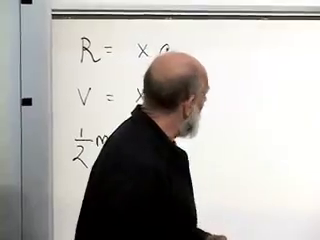
\includegraphics[width=0.72\textwidth]{lecture_09_figure_02.png}
  \caption{Die Metrik des flachen, expandierenden Universums, in der der Skalenfaktor das euklidische räumliche Linienelement multipliziert. Quellbild bei 00:09:12.}
  \label{fig:l09-expanding-metric-board}
\end{figure}

Stellen wir uns Koordinaten vor, die auf ein Gummituch gemalt sind. Die Koordinatenmarkierungen bleiben am Tuch haften, während der physikalische Abstand zwischen ihnen wächst. Eine Koordinatendifferenz wie „von \(x=0\) bis \(x=1\)“ ist also lediglich ein Paar von Bezeichnungen. Der durch dieses Intervall dargestellte Abstand beträgt \(a(t)\). Die Gleichung zu finden, die diesen Skalenfaktor bestimmt, ist das dynamische Problem dieser Vorlesung.

\section{Geschlossene, flache und offene räumliche Geometrien}

Flachheit ist eine beobachtungsbasierte Vereinfachung und folgt nicht aus der Homogenität. Es gibt drei homogene und isotrope räumliche Geometrien: mit positiver, verschwindender und negativer Krümmung. Um den Fall positiver Krümmung zu verstehen, muss man die Dimension genau beachten.

Der geometrische Ort
\begin{equation}
  X_1^2+X_2^2=R^2
\end{equation}
ist ein Kreis oder eine Einsphäre \(S^1\). Sein ausgefülltes Inneres ist eine Kreisscheibe, auch Zweikugel genannt. Fügt man eine Einbettungskoordinate hinzu, erhält man
\begin{equation}
  X_1^2+X_2^2+X_3^2=R^2,
\end{equation}
die gewöhnliche Zweisphäre \(S^2\). Mit einer vierten Einbettungskoordinate erhält man
\begin{equation}
  X_1^2+X_2^2+X_3^2+X_4^2=R^2,
  \label{eq:l09-three-sphere}
\end{equation}
eine Dreisphäre \(S^3\), die selbst ein dreidimensionaler Raum ist. Wir können ihre Einbettung in vier Dimensionen nicht veranschaulichen, doch ihre intrinsische Geometrie benötigt diese Einbettung nicht, um zu existieren.

\begin{figure}[H]
  \centering
  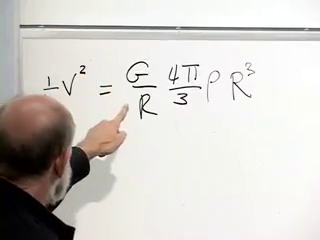
\includegraphics[width=0.72\textwidth]{lecture_09_figure_03.png}
  \caption{Die Einbettungsgleichung, mit der die Dreisphäre eingeführt wird. Quellbild bei
  00:16:40.}
  \label{fig:l09-three-sphere-board}
\end{figure}

Jeder Punkt einer idealen Sphäre ist geometrisch jedem anderen gleichwertig, und an jedem Punkt sind alle Richtungen gleichwertig. Eine Sphäre ist daher sowohl homogen als auch isotrop. Wird ihr Radius mit \(a(t)\) multipliziert, expandiert oder kontrahiert der gesamte Raum, ohne dass dabei ein Mittelpunkt auf der Sphäre ausgezeichnet wird. Verfolgt man die Entwicklung eines solchen Universums rückwärts, befindet sich die gesamte Materie nicht an einem besonderen Ort in einem äußeren, leeren Raum. Vielmehr wird der ganze Raum klein, sodass sich jedes Punktepaar nahekommt. Der Urknall ist keine Explosion von einem einzelnen Punkt des Raums aus.

Auf einer positiv gekrümmten Sphäre beträgt die Winkelsumme in geodätischen Dreiecken mehr als \(180^\circ\). In flachen Dreiecken beträgt die Winkelsumme genau \(180^\circ\). In einer homogenen Geometrie mit negativer Krümmung, die durch eine Sattelfläche nur unvollkommen dargestellt wird, ist die Winkelsumme kleiner als \(180^\circ\). Diese intrinsischen Tests unterscheiden die drei Fälle voneinander.

\begin{figure}[H]
  \centering
  \includegraphics[width=0.72\textwidth]{lecture_09_figure_07.png}
  \caption{Skizze positiver, verschwindender und negativer Krümmung anhand der jeweils charakteristischen Dreiecksformen. Quellbild bei 00:37:30.}
  \label{fig:l09-curvature-board}
\end{figure}

Eine lokal vollkommen flache Metrik beweist für sich genommen nicht, dass der Raum topologisch unendlich ist. Kompakte flache Topologien sind mathematisch möglich, doch in der Vorlesung wird das einfachste Modell eines unendlichen euklidischen Raums verwendet.
\editorialnote{Diese Einschränkung bezüglich der globalen Topologie ist für keine der folgenden lokalen Dynamiken erforderlich.}

\section{Mitbewegte Koordinaten und das Hubble-Gesetz}

Kehren wir nun zum expandierenden flachen Tuch zurück und zeichnen ein Koordinatengitter darauf. In mitbewegten Koordinaten expandiert das Gitter gemeinsam mit der großräumigen Materieströmung. Eine Galaxie oder, genauer gesagt, ein hinreichend grob zusammengefasster Galaxienhaufen behält näherungsweise ihre Koordinatenbezeichnung bei, obwohl sich ihr physikalischer Abstand zu einem anderen mitbewegten Objekt ändert.

\begin{figure}[H]
  \centering
  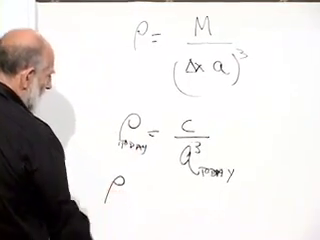
\includegraphics[width=0.72\textwidth]{lecture_09_figure_04.png}
  \caption{Ein Koordinatengitter, das sich mit einem expandierenden räumlichen Tuch mitbewegt.
  Quellbild bei 00:22:20.}
  \label{fig:l09-comoving-grid-board}
\end{figure}

Für zwei Objekte, die entlang der \(x\)-Achse durch ein festes mitbewegtes Intervall \(\Delta x\) getrennt sind, beträgt ihr physikalischer Abstand
\begin{equation}
  D(t)=a(t)\,\Delta x.
  \label{eq:l09-physical-distance}
\end{equation}
Leiten wir ab und halten dabei \(\Delta x\) fest, so erhalten wir
\begin{equation}
  v(t)=\dot a(t)\,\Delta x
      =\frac{\dot a(t)}{a(t)}D(t).
\end{equation}
Definieren wir
\begin{equation}
  H(t)\equiv\frac{\dot a(t)}{a(t)},
  \label{eq:l09-hubble-parameter}
\end{equation}
erhalten wir das Hubble-Gesetz,
\begin{equation}
  v=H(t)D.
  \label{eq:l09-hubble-law}
\end{equation}
Das Wort „konstant“ in „Hubble-Konstante“ bedeutet, dass der Wert zu einem bestimmten kosmischen Zeitpunkt im Raum konstant ist. Es bedeutet nicht, dass er sich im Laufe der kosmischen Geschichte nicht ändert.

\begin{figure}[H]
  \centering
  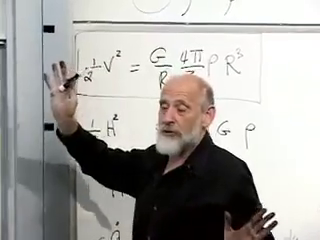
\includegraphics[width=0.72\textwidth]{lecture_09_figure_05.png}
  \caption{Herleitung an der Tafel: \(D=a\Delta x\),
  \(v=(\dot a/a)D=HD\). Quellbild bei 00:26:40.}
  \label{fig:l09-hubble-board}
\end{figure}

\begin{classroomqa}
\audiencequestion{Müsste der aus einer weit entfernten Galaxie ermittelte Hubble-Parameter nicht tatsächlich dem nahebei heute gemessenen Wert entsprechen, wenn wir die Galaxie zu einem früheren Zeitpunkt sehen?}
\lecturerresponse{Nur wenn die Rückblickzeit klein gegenüber dem Alter des Universums ist. Über mäßige Entfernungen ändert sich \(H(t)\) nur wenig, sodass ein einzelner Wert nützlich ist. Bei wirklich kosmologischen Entfernungen sehen wir frühere Epochen; dann müssen die Zeitabhängigkeiten von \(a\) und \(H\) berücksichtigt werden. Das ist ein Grund dafür, dass wir eine dynamische Gleichung für den Skalenfaktor benötigen.}
\end{classroomqa}

\section{Lichtstrahlen in einem expandierenden Koordinatensystem}

\begin{classroomqa}
\audiencequestion{Beeinflusst der Skalenfaktor die Ausbreitung von Licht zwischen weit entfernten Galaxien?}
\lecturerresponse{Ein Lichtstrahl folgt einer lichtartigen Bahn, also gilt \(d\tau=0\). Für einen Strahl, der sich entlang der positiven \(x\)-Achse bewegt, gilt \(dy=dz=0\), und die expandierende Metrik ergibt
\begin{align}
  0&=dt^2-a^2(t)dx^2,
  &dt&=a(t)dx,\notag\\
  &&\frac{dx}{dt}&=\frac{1}{a(t)}.
  \label{eq:l09-null-ray}
\end{align}
Die Koordinatengeschwindigkeit nimmt mit wachsendem \(a(t)\) ab, doch die lokal gemessene Lichtgeschwindigkeit bleibt \(c=1\). Ein festes Koordinatenintervall entspricht einem wachsenden physikalischen Abstand.}
\end{classroomqa}

\begin{figure}[H]
  \centering
  \includegraphics[width=0.72\textwidth]{lecture_09_figure_06.png}
  \caption{Die Nullbedingung und \(dt=a(t)dx\) für die radiale Ausbreitung von Licht.
  Quellbild bei 00:30:54.}
  \label{fig:l09-null-board}
\end{figure}

Man kann Koordinaten wählen, in denen derselbe Sachverhalt wie „Licht wird weiter draußen langsamer“ klingt. Dann werden Längen und Uhren jedoch entsprechend umständlich beschrieben. Die Sprache der expandierenden Räume ist klarer, weil sie die lokale Aussage bewahrt, dass jeder frei fallende Beobachter dieselbe Lichtgeschwindigkeit misst.

\begin{classroomqa}
\audiencequestion{Gibt es Hinweise darauf, dass sich die lokale Lichtausbreitung und die Atomphysik in weit entfernten Galaxien genauso verhalten?}
\lecturerresponse{Operativ sinnvoll sind nur dimensionslose Vergleiche. Man wählt eine atomare Größe als Längeneinheit und eine atomare oder nukleare Periode als Zeiteinheit und fragt dann, wie viele solcher Perioden das Licht benötigt, um die gewählte Länge zu durchqueren. Spektroskopische Beobachtungen stützen die Aussage, dass diese dimensionslosen Verhältnisse in weit entfernten Regionen gleich sind. Die Evidenz ist indirekt, doch genau mit solchen Vergleichen prüft man die Gleichförmigkeit lokaler Naturgesetze.}
\end{classroomqa}

Als das beobachtbare Universum extrem klein war, konnte Licht einen gegebenen physikalischen Bereich, gemessen in der entsprechenden Lichtlaufzeiteinheit, rasch durchqueren. Das bedeutet nicht, dass \(c\) anders war. Es bedeutet, dass der Bereich selbst klein war.

\section{Eine Newtonsche Kugel im Universum}

Nun wenden wir uns von der Kinematik der Dynamik zu. Wir setzen uns in den Ursprung und zeichnen eine Kugel, die groß genug ist, um viele Galaxien und Galaxienhaufen zu umfassen. Auf ihrer Oberfläche wählen wir eine Galaxie aus. In einem homogenen Universum ist die Massenverteilung um uns kugelsymmetrisch, und Newtons Schalentheorem liefert zwei entscheidende Aussagen:
\begin{enumerate}
  \item Die gesamte außerhalb des gewählten Radius kugelsymmetrisch verteilte Materie übt auf die Galaxie an der Kugeloberfläche keine resultierende Newtonsche Kraft aus.
  \item Die gesamte innerhalb der Kugel befindliche Materie wirkt bei dieser radialen Bewegung so, als wäre sie im Mittelpunkt konzentriert.
\end{enumerate}
Wir wählen ein Bezugssystem, in dem wir ruhen; Geschwindigkeiten und Beschleunigungen im folgenden Argument werden also relativ zu uns gemessen.

\begin{figure}[H]
  \centering
  \includegraphics[width=0.72\textwidth]{lecture_09_figure_08.png}
  \caption{Die Konstruktion mit dem Schalentheorem: Wir befinden uns im Mittelpunkt, eine Testgalaxie liegt auf der Oberfläche einer großen homogenen Kugel. Quellbild bei 00:41:10.}
  \label{fig:l09-shell-board}
\end{figure}

\begin{figure}[H]
  \centering
  \begin{tikzpicture}[scale=0.92,>=Latex]
    \draw[thick] (0,0) circle (2.35);
    \fill (0,0) circle (2pt) node[below left] {us};
    \fill (2.35,0) circle (2.2pt) node[right] {test galaxy \(m\)};
    \draw[->,thick,blue!65!black] (0.18,0) -- (2.15,0)
      node[midway,above] {\(R=a(t)x\)};
    \draw[->,thick,red!65!black] (2.35,0.12) -- (3.25,0.12)
      node[midway,above] {\(v=\dot a(t)x\)};
    \node[align=center,text width=7cm] at (0,-2.85)
      {outside shells cancel;\\enclosed mass acts at the center};
  \end{tikzpicture}
  \caption{Saubere Rekonstruktion der Newtonschen Konstruktion.}
  \label{fig:l09-shell-clean}
\end{figure}

Hat die Galaxie die feste mitbewegte Koordinate \(x\), so sind ihr physikalischer Radius und ihre Geschwindigkeit
\begin{equation}
  R(t)=x a(t),
  \qquad
  v(t)=x\dot a(t)=H(t)R(t).
  \label{eq:l09-radius-velocity}
\end{equation}
Sei \(M\) die innerhalb der Kugel eingeschlossene Masse und \(m\) die Masse der Testgalaxie. Die Newtonsche Energie lautet
\begin{equation}
  E=\frac12 m v^2-\frac{GMm}{R}.
  \label{eq:l09-newtonian-energy}
\end{equation}

\begin{figure}[H]
  \centering
  \includegraphics[width=0.72\textwidth]{lecture_09_figure_09.png}
  \caption{Die vollständige Tafelabfolge \(R=xa\), \(v=x\dot a\) und die Newtonsche Energiegleichung für den Spezialfall \(E=0\). Quellbild bei 00:48:40.}
  \label{fig:l09-energy-board}
\end{figure}

Die Energie kann positiv, null oder negativ sein. Wir beginnen mit dem Grenzfall zwischen Entkommen und erneutem Kollaps, \(E=0\), für den gilt
\begin{equation}
  \frac12 v^2=\frac{GM}{R}.
  \label{eq:l09-zero-energy}
\end{equation}

\begin{classroomqa}
\audiencequestion{Was bedeutet eine Gesamtenergie von null für die sich entfernende Galaxie?}
\lecturerresponse{Das ist genau der Fall mit Fluchtgeschwindigkeit. Positive Energie bedeutet eine Bewegung oberhalb der Fluchtgeschwindigkeit; negative Energie bedeutet eine Bewegung unterhalb der Fluchtgeschwindigkeit und führt im Newtonschen Bild mit Materie allein schließlich zur Rückkehr. Wir beginnen an der Grenze zwischen diesen Möglichkeiten und kehren nach der Herleitung der Gleichung für den flachen Fall zu den anderen Vorzeichen zurück.}
\end{classroomqa}

\begin{classroomqa}
\audiencequestion{Ändert sich die eingeschlossene Masse \(M\), wenn sich die Kugel ausdehnt?}
\lecturerresponse{Nein. Die Kugel bewegt sich mit, sodass dieselben Teilchen in ihr bleiben. Ihr physikalisches Volumen wächst und ihre Dichte sinkt, doch ihre gesamte eingeschlossene Masse bleibt konstant. Diese Unterscheidung zwischen \(M\) und \(\rho(t)\) ist wesentlich.}
\end{classroomqa}

Bei einer homogenen Dichte \(\rho(t)\) gilt
\begin{equation}
  M=\frac{4\pi}{3}\rho(t)R^3.
  \label{eq:l09-enclosed-mass}
\end{equation}
Einsetzen in \eqref{eq:l09-zero-energy} ergibt
\begin{equation}
  \frac12 v^2
  =\frac{G}{R}\left(\frac{4\pi}{3}\rho R^3\right).
  \label{eq:l09-enclosed-energy}
\end{equation}

\begin{figure}[H]
  \centering
  \includegraphics[width=0.72\textwidth]{lecture_09_figure_10.png}
  \caption{Einsetzen der eingeschlossenen Masse in die Gleichung für Energie von null.
  Quellbild bei 00:54:16.060.}
  \label{fig:l09-enclosed-mass-board}
\end{figure}

Mit \(v=HR\) erhalten wir
\begin{align}
  \frac12 H^2R^2
    &=\frac{4\pi G}{3}\rho R^2,\\
  H^2
    &=\frac{8\pi G}{3}\rho.
\end{align}
Damit lautet das Expansionsgesetz für den Fall null Energie und räumlicher Flachheit
\begin{equation}
  \boxed{\left(\frac{\dot a}{a}\right)^2
  =\frac{8\pi G}{3}\rho(t)}.
  \label{eq:l09-flat-friedmann}
\end{equation}
Dass sich \(R^2\) herauskürzt, ist kein Zufall. In einem homogenen Universum muss \(H(t)\) denselben Wert haben, unabhängig davon, welche mitbewegte Galaxie als Testobjekt gewählt wurde.

\begin{figure}[H]
  \centering
  \includegraphics[width=0.72\textwidth]{lecture_09_figure_11.png}
  \caption{Die Kürzung des Radius und die daraus folgende Friedmann-Beziehung für den flachen Fall an der Tafel. Quellbild bei 00:57:30.}
  \label{fig:l09-friedmann-board}
\end{figure}

\begin{classroomqa}
\audiencequestion{Gibt es Hinweise auf die Beziehung für den Fall null Energie?}
\lecturerresponse{Beide Seiten lassen sich aus Beobachtungen erschließen: \(H\) aus Daten zur Rezessionsgeschwindigkeit und \(\rho\), indem man Sterne, Gas, Dunkle Materie und Vakuumenergie berücksichtigt. Der Vergleich zur Zeit der Vorlesung ergab, dass beide Seiten auf etwa ein Prozent genau übereinstimmen. Die Einschränkung ist wichtig: Es müssen alle Energieformen berücksichtigt werden, und die spätere Diskussion der Vakuumenergie verändert die naive Deutung anhand der Fluchtgeschwindigkeit.}
\end{classroomqa}

In Einheiten \(c=1\) haben Massendichte und Energiedichte dieselbe Einheit. Das Symbol \(\rho\) bezeichnet daher die gesamte Energiedichte der jeweils betrachteten Komponente.

\section{Gewöhnliche Materie und das Zweidrittelgesetz}

Gleichung \eqref{eq:l09-flat-friedmann} ist erst dann vollständig, wenn wir wissen, wie sich \(\rho(t)\) ändert. Füllen wir zunächst einen mitbewegten Quader mit langsam bewegten, nichtrelativistischen Teilchen. Seine Koordinatenabmessungen bleiben fest, während sein physikalisches Volumen wie folgt wächst:
\begin{equation}
  V(t)=a^3(t)\,\Delta x\,\Delta y\,\Delta z.
\end{equation}
Teilchenzahl und Ruhemasse im Quader bleiben konstant, also gilt
\begin{equation}
  \rho_{\mathrm m}(t)=\frac{C_{\mathrm m}}{a^3(t)}.
  \label{eq:l09-matter-dilution}
\end{equation}
Normiert auf die heutige Epoche \(t_0\) ergibt sich
\begin{equation}
  \frac{\rho_{\mathrm m}(t)}{\rho_{\mathrm m,0}}
  =\left(\frac{a_0}{a(t)}\right)^3.
  \label{eq:l09-matter-normalized}
\end{equation}

\begin{figure}[H]
  \centering
  \includegraphics[width=0.72\textwidth]{lecture_09_figure_12.png}
  \caption{Materiedichte, ihre Abnahme wie \(a^{-3}\) und Normierung auf den heutigen Wert. Quellbild bei 01:04:47.940.}
  \label{fig:l09-density-board}
\end{figure}

\begin{classroomqa}
\audiencequestion{Wie groß ist ungefähr die heutige Energiedichte des Universums, und können gewöhnliche Atome allein sie liefern?}
\lecturerresponse{Eine Zählung der sichtbaren baryonischen Materie liefert nur einen Teil der Antwort. Dunkle Materie und Dunkle Energie müssen ebenfalls als äquivalente Masse-Energie berücksichtigt werden. Die Vorlesung nennt als grobe Größenordnung einen Wert zwischen einem Atom und einigen Dutzend Wasserstoffmassen-Äquivalenten pro Kubikmeter. Dabei geht es um die Größenordnung, nicht um eine präzise Bestandsaufnahme.}
\end{classroomqa}

Setzen wir \eqref{eq:l09-matter-dilution} in \eqref{eq:l09-flat-friedmann} ein und fassen alle zeitunabhängigen Faktoren in einer positiven Konstanten \(C\) zusammen:
\begin{equation}
  \left(\frac{\dot a}{a}\right)^2=\frac{C}{a^3},
  \qquad
  \dot a^2=\frac{C}{a}.
  \label{eq:l09-matter-ode}
\end{equation}
Es gibt zwei anschauliche Lösungswege. Ein Potenzansatz \(a=K t^p\) verlangt
\begin{equation}
  p-1=-\frac{p}{2},
  \qquad p=\frac23.
\end{equation}
Alternativ integrieren wir den expandierenden Ast der Quadratwurzel:
\begin{equation}
  a^{1/2}\frac{da}{dt}=\sqrt C,
  \qquad
  \int a^{1/2}da=\sqrt C\int dt,
\end{equation}
Nach Wahl des Zeitursprungs beim Urknall folgt daher
\begin{equation}
  a^{3/2}\propto t,
  \qquad
  \boxed{a(t)\propto t^{2/3}}.
  \label{eq:l09-matter-solution}
\end{equation}
Bei der Herleitung an der Tafel geht beim Abgleich der Koeffizienten vorübergehend ein Faktor verloren; durch Rückkehr zum Integral wird der Exponent anschließend überprüft. Die Notizen halten diese Kontrolle fest, zeigen aber nur die korrigierte Rechnung.

\begin{figure}[H]
  \centering
  \includegraphics[width=0.72\textwidth]{lecture_09_figure_13.png}
  \caption{Der Potenzansatz und der eingerahmte Exponent \(p=2/3\). Quellbild
  bei 01:13:05.}
  \label{fig:l09-matter-solution-board}
\end{figure}

Durch Ableiten der Lösung erhalten wir
\begin{equation}
  H(t)=\frac{\dot a}{a}=\frac{2}{3t}.
  \label{eq:l09-matter-hubble}
\end{equation}
In der Vergangenheit war der Hubble-Parameter größer. Wenn man also weit genug zurückblickt, um eine beträchtliche Rückblickzeit zu erreichen, sollte man die lokale lineare Beziehung nicht mit dem heutigen Wert von \(H_0\) unverändert fortschreiben.

\begin{figure}[H]
  \centering
  \includegraphics[width=0.72\textwidth]{lecture_09_figure_14.png}
  \caption{Für \(\dot a/a\) und \(a\propto t^{2/3}\) ergibt sich
  \(H=2/(3t)\). Quellbild bei 01:20:42.}
  \label{fig:l09-hubble-time-board}
\end{figure}

\section{Energievorzeichen und räumliche Krümmung}

Mit Newtonscher Argumentation haben wir den flachen Fall mit Gesamtenergie null hergeleitet. Die Allgemeine Relativitätstheorie fügt eine Tatsache hinzu, die sich nicht allein aus dem Schalentheorem gewinnen lässt: Das Vorzeichen der spezifischen Energie im Newtonschen Sinn entspricht dem Vorzeichen der räumlichen Krümmung.
\begin{center}
\begin{tabular}{@{}>{\raggedright\arraybackslash}p{0.20\linewidth}
                    >{\raggedright\arraybackslash}p{0.29\linewidth}
                    >{\raggedright\arraybackslash}p{0.37\linewidth}@{}}
  \toprule
  Gesamt\-energie & Räumliche Krümmung & Entwicklung bei Materie allein \\
  \midrule
  positiv & negativ (offen) & expandiert für immer \\
  null & null (flach) & nähert sich der Fluchtgrenze \\
  negativ & positiv (geschlossen) & expandiert, erreicht einen Umkehrpunkt und kollabiert erneut \\
  \bottomrule
\end{tabular}
\end{center}
Die letzte Spalte setzt Vakuumenergie gleich null voraus. In der Analogie mit einem Geschoss bedeutet positive Energie eine Geschwindigkeit oberhalb der Fluchtgeschwindigkeit, Energie von null genau die Fluchtgeschwindigkeit und negative Energie eine Geschwindigkeit darunter. Einsteins Gleichungen ordnen diesen drei Fällen jeweils eine offene, flache und geschlossene räumliche Geometrie zu.

\section{Photonen und das Halbgesetz}

Das Materiegesetz \(\rho\propto a^{-3}\) setzt voraus, dass die Energie jedes Teilchens näherungsweise konstant bleibt, während die Teilchenzahldichte abnimmt. Für Photonen gilt diese Annahme nicht. Für ein Photon gilt
\begin{equation}
  E=h\nu=\frac{hc}{\lambda}.
\end{equation}
Durch die Expansion wird seine Wellenlänge proportional zum Skalenfaktor gestreckt:
\begin{equation}
  \lambda\propto a,
  \qquad E\propto a^{-1}.
\end{equation}
Die Photonenzahldichte nimmt weiterhin wie \(a^{-3}\) ab, und die Energie jedes Photons bringt einen zusätzlichen Faktor \(a^{-1}\) ein. Daher gilt
\begin{equation}
  \boxed{\rho_{\mathrm r}(t)\propto a^{-4}(t)}.
  \label{eq:l09-radiation-dilution}
\end{equation}

Die Analogie mit einer Gitarrensaite veranschaulicht das physikalische Bild. Zupft man eine Saite an und verlängert dann den schwingenden Abschnitt, wird die Wellenlänge größer und der Ton tiefer. Eine Photonenmode in einem expandierenden mitbewegten Kasten verhält sich ähnlich. Betrachtet man den Vorgang rückwärts, verkürzt die Kompression die Wellenlängen und erhöht die Photonenergien.

\begin{figure}[H]
  \centering
  \includegraphics[width=0.72\textwidth]{lecture_09_figure_15.png}
  \caption{Die Beziehung für die Materiedichte wird an der Tafel auf die Skalierung der Strahlung \(\rho_{\mathrm r}\propto a^{-4}\) erweitert. Quellbild bei 01:29:20.}
  \label{fig:l09-radiation-board}
\end{figure}

Setzen wir \(\rho_{\mathrm r}\propto a^{-4}\) in die Friedmann-Gleichung für den flachen Fall ein, erhalten wir
\begin{equation}
  \left(\frac{\dot a}{a}\right)^2=\frac{C_{\mathrm r}}{a^4},
  \qquad
  \dot a\propto a^{-1},
\end{equation}
und damit
\begin{equation}
  \boxed{a(t)\propto t^{1/2}}.
  \label{eq:l09-radiation-solution}
\end{equation}
Das wächst langsamer als \(t^{2/3}\). Weit genug in der Vergangenheit muss die Strahlung gegenüber gewöhnlicher Materie dominieren, denn \(a^{-4}\) nimmt bei abnehmendem \(a\) schneller zu als \(a^{-3}\). Der Übergang zwischen Materie- und Strahlungsdominanz liegt der Vorlesung zufolge ungefähr in der Epoche, in der der Skalenfaktor etwa tausendmal kleiner war als heute. Davor dominierte die Strahlung, danach über einen langen Zeitraum die Materie.

\section{Vakuumenergie und exponentielle Expansion}

Vakuumenergie skaliert entgegengesetzt. Ihre Dichte ist eine Eigenschaft des leeren Raums und nimmt bei der Expansion des Universums nicht ab:
\begin{equation}
  \rho_\Lambda=\text{constant}.
  \label{eq:l09-vacuum-density}
\end{equation}
Gewöhnliche Materie und Strahlung werden in der Vergangenheit dichter, während dieser Beitrag sich nicht ändert. Deshalb war er im frühen Universum weniger wichtig und gewinnt an Bedeutung, wenn die anderen Komponenten verdünnt werden. Die Vorlesung verwendet die damalige Schätzung, dass Vakuumenergie etwa \(70\%\) der heutigen kosmischen Energiedichte ausmacht.

Bei konstantem \(\rho_\Lambda\) ergibt Gleichung \eqref{eq:l09-flat-friedmann} eine konstante Expansionsrate:
\begin{equation}
  H_\Lambda=\sqrt{\frac{8\pi G}{3}\rho_\Lambda},
  \qquad
  \frac{\dot a}{a}=H_\Lambda.
\end{equation}
Daher gilt
\begin{equation}
  \boxed{a(t)=a(t_i)e^{H_\Lambda(t-t_i)}}.
  \label{eq:l09-vacuum-solution}
\end{equation}

\begin{figure}[H]
  \centering
  \includegraphics[width=0.72\textwidth]{lecture_09_figure_16.png}
  \caption{Die Gleichung mit konstanter Dichte führt zur exponentiellen Expansion.
  Quellbild bei 01:35:48.}
  \label{fig:l09-vacuum-board}
\end{figure}

Bei der in der Vorlesung genannten beobachteten Größenordnung verdoppelt sich die lineare Größe des Universums in etwa zehn bis zwölf Milliarden Jahren. Der Ursprung dieser kleinen, aber von null verschiedenen Vakuumdichte ist weiterhin ungeklärt; ihre Existenz und ihre Wirkung auf die Expansion sind empirische Tatsachen.

\begin{classroomqa}
\audiencequestion{Ist Vakuumenergie in dieser Diskussion dasselbe wie Dunkle Energie?}
\lecturerresponse{Ja. Hier bezeichnet „Dunkle Energie“ eine konstante Vakuumenergiedichte, gleichbedeutend mit einer kosmologischen Konstante. Allgemeinere Modelle mit zeitabhängiger Dunkler Energie sind denkbar, gehören aber nicht zu den Berechnungen dieser Vorlesung.}
\end{classroomqa}

\section{Wie die Expansion des Universums Licht rotverschiebt}

\begin{classroomqa}
\audiencequestion{Wie können Photonen wissen, dass wir expandierende mitbewegte Koordinaten gewählt haben, und deshalb ihre Energie verringern?}
\lecturerresponse{Sie reagieren nicht auf unsere Koordinatenbezeichnungen. Sie breiten sich durch eine Geometrie aus, in der sich die physikalischen Abstände ändern. Ein Wellenzug, der einen Bereich einnimmt, dessen physikalische Größe sich verdoppelt, erhält die doppelte Wellenlänge. Die mitbewegten Koordinaten beschreiben diese Streckung lediglich auf ökonomische Weise; sie verursachen sie nicht.}
\end{classroomqa}

\begin{classroomqa}
\audiencequestion{Woher stammen die Hintergrundphotonen, die uns heute erreichen?}
\lecturerresponse{Je weiter wir in die Ferne blicken, desto weiter blicken wir in die Vergangenheit. Schließlich sehen wir die Epoche, in der das kosmische Material ein ionisiertes Plasma war, undurchsichtig, weil Photonen wiederholt an freien geladenen Teilchen gestreut wurden. Die Grenze, von der aus Photonen zuletzt ungehindert zu uns gelangen konnten, erscheint als eine den Beobachter umgebende Kugel: die Oberfläche der letzten Streuung.}
\end{classroomqa}

\begin{figure}[H]
  \centering
  \includegraphics[width=0.72\textwidth]{lecture_09_figure_17.png}
  \caption{Skizze der beobachterzentrierten Oberfläche der letzten Streuung und immer weiter entfernter Schalen. Quellbild bei 01:42:05.}
  \label{fig:l09-last-scattering-board}
\end{figure}

\begin{figure}[H]
  \centering
  \begin{tikzpicture}[scale=0.9,>=Latex]
    \fill (0,0) circle (2pt) node[below] {observer};
    \draw[thick,orange!70!black] (0,0) circle (2.55);
    \node[orange!70!black,align=center] at (0,3.05)
      {surface of last scattering};
    \foreach \a in {25,75,145,210,285,335}{
      \draw[->,blue!60!black] ({2.55*cos(\a)},{2.55*sin(\a)}) --
        ({1.7*cos(\a)},{1.7*sin(\a)});
    }
    \draw[decorate,decoration={snake,amplitude=1.5pt,segment length=7pt},
      red!65!black,thick,->] (-2.5,0) -- (-0.15,0);
    \node[red!65!black,below] at (-1.35,-0.15)
      {redshifted photon};
  \end{tikzpicture}
  \caption{Saubere Rekonstruktion der Darstellung der letzten Streuung.}
  \label{fig:l09-last-scattering-clean}
\end{figure}

Die Strahlung wurde mit einem für heißes Plasma charakteristischen Spektrum emittiert und erreicht uns mit Wellenlängen, die ungefähr tausendmal länger sind. In der Doppler-Sprache der Vorlesung entfernt sich die weit entfernte emittierende Oberfläche rasch, sodass ihre Strahlung stark rotverschoben ist. In der geometrischen Beschreibung wird die Welle während ihrer Ausbreitung gestreckt. Beide Bilder drücken denselben Zusammenhang aus:
\begin{equation}
  1+z=\frac{\lambda_0}{\lambda_{\mathrm{em}}}
      =\frac{a_0}{a_{\mathrm{em}}}.
  \label{eq:l09-cosmological-redshift}
\end{equation}
\editorialnote{Gleichung \eqref{eq:l09-cosmological-redshift} ist die übliche quantitative Form der Streckungs- und Doppler-Beschreibungen aus der Vorlesung.}

Zu einer früheren Beobachtungsepoche wäre die Oberfläche der letzten Streuung im entsprechenden Bild näher gewesen; die beobachteten Hintergrundphotonen wären weniger rotverschoben und damit energiereicher gewesen. Mit fortschreitender kosmischer Zeit haben die Photonen, die einen mitbewegten Beobachter aus jenem frühen Plasma erreichen, immer längere Wellenlängen.

\section{Wohin geht die Energie eines rotverschobenen Photons?}

\begin{classroomqa}
\audiencequestion{Ein Photon wird mit der Energie \(h\nu_{\mathrm{em}}\) emittiert und kommt rotverschoben mit geringerer Energie an. Was ist mit der Energiedifferenz geschehen?}
\lecturerresponse{Die Newtonsche Herleitung begann mit einer Energiegleichung. Ihre kosmologische Form verknüpft die Expansionsrate mit der Energie­dichte der Materie, sodass Materieenergie und Expansion nicht als unabhängig voneinander erhaltene Größen behandelt werden können. Der Vorlesung zufolge geht die verlorene Photonenenergie in die Energiebilanz der Expansion ein. Ein mit Strahlung gefüllter Kolben veranschaulicht die Analogie: Der Strahlungsdruck schiebt den Kolben nach außen, die Photonenwellenlängen nehmen zu, und ihre verlorene Energie wird zu mechanischer Arbeit und kinetischer Energie des Kolbens.}
\end{classroomqa}

\begin{figure}[H]
  \centering
  \includegraphics[width=0.72\textwidth]{lecture_09_figure_18.png}
  \caption{Die eingerahmte Newtonsche Energiegleichung steht an der Tafel über der entsprechenden Friedmann-Gleichung. Quellbild bei 01:44:42.}
  \label{fig:l09-energy-bookkeeping-board}
\end{figure}

\begin{classroomqa}
\audiencequestion{Was koppelt die Strahlungsenergie an die Expansion?}
\lecturerresponse{Der Druck. In einem Zylinder mit beweglichem Kolben übertragen Photonen Impuls auf die Wand. Bewegt sich der Kolben, verrichtet die Strahlung Arbeit; ihre Wellenlänge wächst und ihre Energie nimmt ab. Das homogene expandierende Universum hat keinen tatsächlichen äußeren Kolben, doch die Analogie mit \(p\,dV\) erklärt, warum die Energiedichte der Strahlung schneller abnimmt, als es allein durch die abnehmende Teilchenzahldichte der Fall wäre.}
\end{classroomqa}

\begin{figure}[H]
  \centering
  \includegraphics[width=0.72\textwidth]{lecture_09_figure_19.png}
  \caption{Der bewegliche, mit Photonen gefüllte Kolben veranschaulicht die Druckarbeit.
  Quellbild bei 01:46:40.}
  \label{fig:l09-piston-board}
\end{figure}

\begin{figure}[H]
  \centering
  \begin{tikzpicture}[scale=0.92,>=Latex]
    \draw[thick] (0,0) rectangle (5.3,2.6);
    \draw[very thick] (4.25,0) -- (4.25,2.6);
    \draw[very thick] (4.25,1.3) -- (5.25,1.3);
    \draw[->,thick,red!65!black] (5.25,1.3) -- (6.2,1.3)
      node[right] {moving piston};
    \foreach \y in {0.55,1.3,2.05}{
      \draw[decorate,decoration={snake,amplitude=1.4pt,segment length=6pt},
        blue!65!black,->] (0.35,\y) -- (3.9,\y);
    }
    \node at (2.15,-0.45) {radiation does \(p\,dV\) work};
  \end{tikzpicture}
  \caption{Saubere Rekonstruktion der Kolbenanalogie für Strahlung.}
  \label{fig:l09-piston-clean}
\end{figure}

Energie erfordert in der allgemeinen Relativitätstheorie besondere Sorgfalt. In einer allgemeinen expandierenden Raumzeit muss es keine eindeutige globale Erhaltungsgröße geben, die der Energie eines isolierten Newtonschen Systems entspricht. Die lokale Erhaltung des Energie-Impuls-Tensors gilt weiterhin; für ein homogenes Fluid führt sie zur Kontinuitätsgleichung
\begin{equation}
  \dot\rho+3H(\rho+p)=0,
  \label{eq:l09-continuity}
\end{equation}
Sie enthält den Druckarbeits-Term, der den Skalierungsgesetzen für Materie und Strahlung zugrunde liegt.\editorialnote{Gleichung \eqref{eq:l09-continuity} ist die präzise lokale Aussage der allgemeinen Relativitätstheorie, auf der die bewusst Newtonsche Analogie der Vorlesung zur Energiebilanz beruht.}

Vakuumenergie macht das Rätsel besonders deutlich. Da ihre Dichte konstant bleibt, während das Volumen wächst, nimmt die gesamte Vakuumenergie in einem mitbewegten Gebiet zu. Ihr negativer Druck ist Teil der Gravitationsquelle und treibt die beschleunigte Expansion an. Man sollte daher nicht die separate Erhaltung der naiven „Materieenergie in einem mitbewegten Kasten“ fordern, ohne Geometrie und Druckarbeit einzubeziehen.

\section{Warum sich der Skalenfaktor aus dem Zeitterm entfernen lässt}

\begin{classroomqa}
\audiencequestion{Warum multipliziert der Skalenfaktor den räumlichen Teil der Metrik, aber nicht den zeitlichen?}
\lecturerresponse{Das ist eine Wahl der Zeitkoordinate. Nehmen wir an, man beginnt mit der konformen Zeitkoordinate \(t\), für die gilt:
\begin{equation}
  d\tau^2=A^2(t)\left(dt^2-dx^2\right).
\end{equation}
Nun definieren wir eine neue kosmische Zeit \(T\) durch
\begin{equation}
  dT=A(t)\,dt.
\end{equation}
Dann gilt:
\begin{equation}
  d\tau^2=dT^2-A^2\bigl(t(T)\bigr)dx^2.
\end{equation}
Der gemeinsame Faktor vor dem Zeitdifferential ist verschwunden, während der physikalische Skalenfaktor im räumlichen Term erhalten bleibt.}
\end{classroomqa}

\begin{figure}[H]
  \centering
  \includegraphics[width=0.72\textwidth]{lecture_09_figure_20.png}
  \caption{Die Zeitumparametrisierung \(dT=A(t)dt\), mit der konforme Zeit in kosmische Zeit umgewandelt wird. Quellbild bei 01:51:05.}
  \label{fig:l09-time-reparam-board}
\end{figure}

\section{Krümmung, Vakuumenergie und das Schicksal des Kosmos}

\begin{classroomqa}
\audiencequestion{Wenn das Universum positiv gekrümmt wäre, müssten wir dann nicht bereits Galaxien auf uns zukommen sehen?}
\lecturerresponse{Nicht unbedingt. Ein Geschoss, das mit einer Geschwindigkeit unterhalb der Fluchtgeschwindigkeit gestartet wird, bewegt sich zunächst nach außen, erreicht einen Umkehrpunkt und fällt erst danach zurück. Wir beobachten das Universum während einer Expansionsphase. Ohne Vakuumenergie würde ein positiv gekrümmtes, von Materie dominiertes Universum schließlich wieder kollabieren. Eine hinreichend große positive Vakuumenergie verhindert diese Umkehr, und ihr beobachteter Wert scheint groß genug zu sein, um die Expansion langfristig unabhängig von einer geringen räumlichen Krümmung exponentiell werden zu lassen.}
\end{classroomqa}

Die exponentielle Zukunft ist kein energetisches Paradies. Sterne erlöschen schließlich, die Dichten von Materie und Strahlung nehmen exponentiell ab, und weit voneinander entfernte Gebiete verlieren den kausalen Kontakt. Die Vakuumenergie bleibt bestehen, während gewöhnliche Strukturen zunehmend kälter und dünner verteilt werden.

\begin{classroomqa}
\audiencequestion{Gibt es in der weiter zurückliegenden Vergangenheit mehr Photonen als gewöhnliche Teilchen?}
\lecturerresponse{Das Verhältnis der Photonenzahl zur Baryonenzahl ist bereits enorm; in der Schätzung der Vorlesung kommen ungefähr \(10^{10}\) Photonen auf ein Baryon. Beide Zahlen bleiben in einem mitbewegten Volumen näherungsweise konstant. In der Vergangenheit ändert sich vor allem die Energie pro Photon. Die Photonenergien steigen wie \(a^{-1}\), die Ruhemasse nichtrelativistischer Teilchen dagegen nicht. Daher dominiert Strahlung zu frühen Zeiten die Energiedichte, auch wenn sich das Zahlenverhältnis selbst nicht ändern muss.}
\end{classroomqa}

Die zentrale Erkenntnis lautet, dass die Geometrie allein die kosmische Entwicklung nicht bestimmt. Die flache Friedmann-Gleichung stellt den Zusammenhang zwischen Expansion und Energiedichte her, doch der Materieinhalt bestimmt deren zeitliche Entwicklung. Nichtrelativistische Materie ergibt \(a\propto t^{2/3}\), Strahlung ergibt \(a\propto t^{1/2}\), und konstante Vakuumenergie führt zu exponentieller Expansion. Diese drei Gesetze ordnen die aufeinanderfolgenden Epochen des Universums und erklären, warum derselbe Skalenfaktor Abstände, Rotverschiebungen und den sich ändernden Hubble-Parameter bestimmt.

\end{document}